% Options for packages loaded elsewhere
\PassOptionsToPackage{unicode}{hyperref}
\PassOptionsToPackage{hyphens}{url}
\PassOptionsToPackage{dvipsnames,svgnames,x11names}{xcolor}
%
\documentclass[
  letterpaper,
  DIV=11,
  numbers=noendperiod]{scrreprt}

\usepackage{amsmath,amssymb}
\usepackage{iftex}
\ifPDFTeX
  \usepackage[T1]{fontenc}
  \usepackage[utf8]{inputenc}
  \usepackage{textcomp} % provide euro and other symbols
\else % if luatex or xetex
  \usepackage{unicode-math}
  \defaultfontfeatures{Scale=MatchLowercase}
  \defaultfontfeatures[\rmfamily]{Ligatures=TeX,Scale=1}
\fi
\usepackage{lmodern}
\ifPDFTeX\else  
    % xetex/luatex font selection
\fi
% Use upquote if available, for straight quotes in verbatim environments
\IfFileExists{upquote.sty}{\usepackage{upquote}}{}
\IfFileExists{microtype.sty}{% use microtype if available
  \usepackage[]{microtype}
  \UseMicrotypeSet[protrusion]{basicmath} % disable protrusion for tt fonts
}{}
\makeatletter
\@ifundefined{KOMAClassName}{% if non-KOMA class
  \IfFileExists{parskip.sty}{%
    \usepackage{parskip}
  }{% else
    \setlength{\parindent}{0pt}
    \setlength{\parskip}{6pt plus 2pt minus 1pt}}
}{% if KOMA class
  \KOMAoptions{parskip=half}}
\makeatother
\usepackage{xcolor}
\setlength{\emergencystretch}{3em} % prevent overfull lines
\setcounter{secnumdepth}{5}
% Make \paragraph and \subparagraph free-standing
\ifx\paragraph\undefined\else
  \let\oldparagraph\paragraph
  \renewcommand{\paragraph}[1]{\oldparagraph{#1}\mbox{}}
\fi
\ifx\subparagraph\undefined\else
  \let\oldsubparagraph\subparagraph
  \renewcommand{\subparagraph}[1]{\oldsubparagraph{#1}\mbox{}}
\fi

\usepackage{color}
\usepackage{fancyvrb}
\newcommand{\VerbBar}{|}
\newcommand{\VERB}{\Verb[commandchars=\\\{\}]}
\DefineVerbatimEnvironment{Highlighting}{Verbatim}{commandchars=\\\{\}}
% Add ',fontsize=\small' for more characters per line
\usepackage{framed}
\definecolor{shadecolor}{RGB}{241,243,245}
\newenvironment{Shaded}{\begin{snugshade}}{\end{snugshade}}
\newcommand{\AlertTok}[1]{\textcolor[rgb]{0.68,0.00,0.00}{#1}}
\newcommand{\AnnotationTok}[1]{\textcolor[rgb]{0.37,0.37,0.37}{#1}}
\newcommand{\AttributeTok}[1]{\textcolor[rgb]{0.40,0.45,0.13}{#1}}
\newcommand{\BaseNTok}[1]{\textcolor[rgb]{0.68,0.00,0.00}{#1}}
\newcommand{\BuiltInTok}[1]{\textcolor[rgb]{0.00,0.23,0.31}{#1}}
\newcommand{\CharTok}[1]{\textcolor[rgb]{0.13,0.47,0.30}{#1}}
\newcommand{\CommentTok}[1]{\textcolor[rgb]{0.37,0.37,0.37}{#1}}
\newcommand{\CommentVarTok}[1]{\textcolor[rgb]{0.37,0.37,0.37}{\textit{#1}}}
\newcommand{\ConstantTok}[1]{\textcolor[rgb]{0.56,0.35,0.01}{#1}}
\newcommand{\ControlFlowTok}[1]{\textcolor[rgb]{0.00,0.23,0.31}{#1}}
\newcommand{\DataTypeTok}[1]{\textcolor[rgb]{0.68,0.00,0.00}{#1}}
\newcommand{\DecValTok}[1]{\textcolor[rgb]{0.68,0.00,0.00}{#1}}
\newcommand{\DocumentationTok}[1]{\textcolor[rgb]{0.37,0.37,0.37}{\textit{#1}}}
\newcommand{\ErrorTok}[1]{\textcolor[rgb]{0.68,0.00,0.00}{#1}}
\newcommand{\ExtensionTok}[1]{\textcolor[rgb]{0.00,0.23,0.31}{#1}}
\newcommand{\FloatTok}[1]{\textcolor[rgb]{0.68,0.00,0.00}{#1}}
\newcommand{\FunctionTok}[1]{\textcolor[rgb]{0.28,0.35,0.67}{#1}}
\newcommand{\ImportTok}[1]{\textcolor[rgb]{0.00,0.46,0.62}{#1}}
\newcommand{\InformationTok}[1]{\textcolor[rgb]{0.37,0.37,0.37}{#1}}
\newcommand{\KeywordTok}[1]{\textcolor[rgb]{0.00,0.23,0.31}{#1}}
\newcommand{\NormalTok}[1]{\textcolor[rgb]{0.00,0.23,0.31}{#1}}
\newcommand{\OperatorTok}[1]{\textcolor[rgb]{0.37,0.37,0.37}{#1}}
\newcommand{\OtherTok}[1]{\textcolor[rgb]{0.00,0.23,0.31}{#1}}
\newcommand{\PreprocessorTok}[1]{\textcolor[rgb]{0.68,0.00,0.00}{#1}}
\newcommand{\RegionMarkerTok}[1]{\textcolor[rgb]{0.00,0.23,0.31}{#1}}
\newcommand{\SpecialCharTok}[1]{\textcolor[rgb]{0.37,0.37,0.37}{#1}}
\newcommand{\SpecialStringTok}[1]{\textcolor[rgb]{0.13,0.47,0.30}{#1}}
\newcommand{\StringTok}[1]{\textcolor[rgb]{0.13,0.47,0.30}{#1}}
\newcommand{\VariableTok}[1]{\textcolor[rgb]{0.07,0.07,0.07}{#1}}
\newcommand{\VerbatimStringTok}[1]{\textcolor[rgb]{0.13,0.47,0.30}{#1}}
\newcommand{\WarningTok}[1]{\textcolor[rgb]{0.37,0.37,0.37}{\textit{#1}}}

\providecommand{\tightlist}{%
  \setlength{\itemsep}{0pt}\setlength{\parskip}{0pt}}\usepackage{longtable,booktabs,array}
\usepackage{calc} % for calculating minipage widths
% Correct order of tables after \paragraph or \subparagraph
\usepackage{etoolbox}
\makeatletter
\patchcmd\longtable{\par}{\if@noskipsec\mbox{}\fi\par}{}{}
\makeatother
% Allow footnotes in longtable head/foot
\IfFileExists{footnotehyper.sty}{\usepackage{footnotehyper}}{\usepackage{footnote}}
\makesavenoteenv{longtable}
\usepackage{graphicx}
\makeatletter
\def\maxwidth{\ifdim\Gin@nat@width>\linewidth\linewidth\else\Gin@nat@width\fi}
\def\maxheight{\ifdim\Gin@nat@height>\textheight\textheight\else\Gin@nat@height\fi}
\makeatother
% Scale images if necessary, so that they will not overflow the page
% margins by default, and it is still possible to overwrite the defaults
% using explicit options in \includegraphics[width, height, ...]{}
\setkeys{Gin}{width=\maxwidth,height=\maxheight,keepaspectratio}
% Set default figure placement to htbp
\makeatletter
\def\fps@figure{htbp}
\makeatother

\usepackage{array}
\usepackage{caption}
\usepackage{graphicx}
\usepackage{siunitx}
\usepackage[normalem]{ulem}
\usepackage{colortbl}
\usepackage{multirow}
\usepackage{hhline}
\usepackage{calc}
\usepackage{tabularx}
\usepackage{threeparttable}
\usepackage{wrapfig}
\usepackage{adjustbox}
\usepackage{hyperref}
\KOMAoption{captions}{tableheading}
\makeatletter
\makeatother
\makeatletter
\@ifpackageloaded{bookmark}{}{\usepackage{bookmark}}
\makeatother
\makeatletter
\@ifpackageloaded{caption}{}{\usepackage{caption}}
\AtBeginDocument{%
\ifdefined\contentsname
  \renewcommand*\contentsname{Table of contents}
\else
  \newcommand\contentsname{Table of contents}
\fi
\ifdefined\listfigurename
  \renewcommand*\listfigurename{List of Figures}
\else
  \newcommand\listfigurename{List of Figures}
\fi
\ifdefined\listtablename
  \renewcommand*\listtablename{List of Tables}
\else
  \newcommand\listtablename{List of Tables}
\fi
\ifdefined\figurename
  \renewcommand*\figurename{Figure}
\else
  \newcommand\figurename{Figure}
\fi
\ifdefined\tablename
  \renewcommand*\tablename{Table}
\else
  \newcommand\tablename{Table}
\fi
}
\@ifpackageloaded{float}{}{\usepackage{float}}
\floatstyle{ruled}
\@ifundefined{c@chapter}{\newfloat{codelisting}{h}{lop}}{\newfloat{codelisting}{h}{lop}[chapter]}
\floatname{codelisting}{Listing}
\newcommand*\listoflistings{\listof{codelisting}{List of Listings}}
\makeatother
\makeatletter
\@ifpackageloaded{caption}{}{\usepackage{caption}}
\@ifpackageloaded{subcaption}{}{\usepackage{subcaption}}
\makeatother
\makeatletter
\@ifpackageloaded{tcolorbox}{}{\usepackage[skins,breakable]{tcolorbox}}
\makeatother
\makeatletter
\@ifundefined{shadecolor}{\definecolor{shadecolor}{rgb}{.97, .97, .97}}
\makeatother
\makeatletter
\makeatother
\makeatletter
\makeatother
\ifLuaTeX
\usepackage[bidi=basic]{babel}
\else
\usepackage[bidi=default]{babel}
\fi
% get rid of language-specific shorthands (see #6817):
\let\LanguageShortHands\languageshorthands
\def\languageshorthands#1{}
\ifLuaTeX
  \usepackage{selnolig}  % disable illegal ligatures
\fi
\IfFileExists{bookmark.sty}{\usepackage{bookmark}}{\usepackage{hyperref}}
\IfFileExists{xurl.sty}{\usepackage{xurl}}{} % add URL line breaks if available
\urlstyle{same} % disable monospaced font for URLs
\hypersetup{
  pdftitle={臨床薬理に関する解析用標準プログラムの作成},
  pdfauthor={CDISC Japan User Group/ADaM therma 3},
  pdflang={jp},
  colorlinks=true,
  linkcolor={blue},
  filecolor={Maroon},
  citecolor={Blue},
  urlcolor={Blue},
  pdfcreator={LaTeX via pandoc}}

\title{臨床薬理に関する解析用標準プログラムの作成}
\author{CDISC Japan User Group/ADaM therma 3}
\date{2024-01-11}

\begin{document}
\maketitle
\ifdefined\Shaded\renewenvironment{Shaded}{\begin{tcolorbox}[breakable, frame hidden, interior hidden, borderline west={3pt}{0pt}{shadecolor}, sharp corners, boxrule=0pt, enhanced]}{\end{tcolorbox}}\fi

\renewcommand*\contentsname{Table of contents}
{
\hypersetup{linkcolor=}
\setcounter{tocdepth}{2}
\tableofcontents
}
\bookmarksetup{startatroot}

\hypertarget{ux7528ux8a9eux7565ux8a9e}{%
\chapter{用語・略語}\label{ux7528ux8a9eux7565ux8a9e}}

\bookmarksetup{startatroot}

\hypertarget{ux306fux3058ux3081ux306b}{%
\chapter{はじめに}\label{ux306fux3058ux3081ux306b}}

申請時にCDISC標準形式での提出の義務化に伴い、臨床薬理評価を含む試験がより複雑なプロセスを生み、各社試行錯誤の対応がなされている。プロセスは複雑ではあるものの、ADNCAやADPPKなどの統一された解析データセットの普及が進むことで、属人性の脱却や臨床薬理結果の再現性の担保などが期待される。

臨床薬理領域の専門家はRプログラム言語を用いた解析結果の作成をしているが、生物統計解析業務やCDISC標準業務ではSASプログラム言語がデファクトスタンダードである。しかし、近年FDAでRプログラム言語を用いた電子申請のパイロット試験の実施を境に、Rプログラム言語への関心が高まっている。

これまでCJUG
ADaMの臨床薬理チームは、NCAにおけるSDTM・ADaMのワークフロー提案を行ってきたが、具体的な処理手順の詳細には踏み込んでいなかった。上記の状況を加味し、昨年からRプログラム言語を使用した標準的な解析プログラムのテンプレート化を進めている。今年度のタスクとしてプログラムのテスト実行と、その使用手順を明記したドキュメントの作成(Github
Pagesによるインストラクション)を進めている。

\bookmarksetup{startatroot}

\hypertarget{rux30d7ux30edux30b0ux30e9ux30e0ux306eux958bux767aux74b0ux5883ux3068ux305dux306eux5468ux8fba}{%
\chapter{Rプログラムの開発環境とその周辺}\label{rux30d7ux30edux30b0ux30e9ux30e0ux306eux958bux767aux74b0ux5883ux3068ux305dux306eux5468ux8fba}}

Rstudioとgitを用いた開発環境を前提とする。

\hypertarget{server-or-desktop}{%
\subsection{server or desktop}\label{server-or-desktop}}

\begin{enumerate}
\def\labelenumi{\arabic{enumi}.}
\tightlist
\item
  Rstudio Server

  \begin{enumerate}
  \def\labelenumii{\arabic{enumii}.}
  \tightlist
  \item
    サーバー環境下
  \item
    仮想環境下
  \end{enumerate}
\item
  Rstudio Desktop
\end{enumerate}

\hypertarget{ux30d1ux30c3ux30b1ux30fcux30b8ux7ba1ux7406}{%
\subsection{パッケージ管理}\label{ux30d1ux30c3ux30b1ux30fcux30b8ux7ba1ux7406}}

\begin{enumerate}
\def\labelenumi{\arabic{enumi}.}
\tightlist
\item
  rproject
\item
  renv
\item
  checkpoint
\end{enumerate}

\hypertarget{ux63a8ux5968ux521dux671fux8a2dux5b9a}{%
\subsection{推奨初期設定}\label{ux63a8ux5968ux521dux671fux8a2dux5b9a}}

\begin{enumerate}
\def\labelenumi{\arabic{enumi}.}
\tightlist
\item
  pacman
\item
  rio
\item
  tidyverse
\end{enumerate}

\bookmarksetup{startatroot}

\hypertarget{tidyverseux306eux8aacux660e}{%
\chapter{Tidyverseの説明}\label{tidyverseux306eux8aacux660e}}

\url{https://uribo.github.io/230827ism_ws/}

\hypertarget{dplyrux306eux8aacux660e}{%
\subsection{dplyrの説明}\label{dplyrux306eux8aacux660e}}

\hypertarget{tidyrux306eux8aacux660e}{%
\subsection{tidyrの説明}\label{tidyrux306eux8aacux660e}}

\bookmarksetup{startatroot}

\hypertarget{adncaux306eux5909ux6570ux306eux8aacux660e}{%
\chapter{ADNCAの変数の説明}\label{adncaux306eux5909ux6570ux306eux8aacux660e}}

絶賛更新中

\bookmarksetup{startatroot}

\hypertarget{adncaux306eux4f5cux4f8bux624bux9806}{%
\chapter{ADNCAの作例手順}\label{adncaux306eux4f5cux4f8bux624bux9806}}

\begin{Shaded}
\begin{Highlighting}[]
\CommentTok{\# CRAN から入手可能なパッケージ}
\DocumentationTok{\#\#\#\#\#\#\#\#\#\#\#\#\#\#\#\#\#\#\#\#\#\#\#\#\#\#\#\#\#\#}
\NormalTok{pacman}\SpecialCharTok{::}\FunctionTok{p\_load}\NormalTok{(}
  \CommentTok{\# 一般的なデータ管理}
  \DocumentationTok{\#\#\#\#\#\#\#\#\#\#\#\#\#\#\#\#\#\#\#\#}
\NormalTok{  tidyverse, }
\NormalTok{  magrittr, }
  
  \CommentTok{\# パッケージのインストールと管理}
  \DocumentationTok{\#\#\#\#\#\#\#\#\#\#\#\#\#\#\#\#\#\#\#\#\#\#\#\#\#\#\#\#\#\#\#\#}
\NormalTok{  pacman,   }\CommentTok{\# パッケージのインストール・読み込み}
\NormalTok{  renv,     }\CommentTok{\# グループで作業する際のパッケージのバージョン管理  }
  
  \CommentTok{\# プロジェクトとファイルの管理}
  \DocumentationTok{\#\#\#\#\#\#\#\#\#\#\#\#\#\#\#\#\#\#\#\#\#\#\#\#\#\#\#\#\#\#}
\NormalTok{  here,     }\CommentTok{\# Rのプロジェクトフォルダを基準とするファイルパス}
\NormalTok{  rio,      }\CommentTok{\# 様々なタイプのデータのインポート・エクスポート}
  
  \CommentTok{\# admiral関連パッケージ}
  \DocumentationTok{\#\#\#\#\#\#\#\#\#\#\#\#\#\#\#\#\#\#\#\#\#\#\#\#\#\#\#\#\#\#\#\#}
\NormalTok{  admiral, }\CommentTok{\# シミュレーション/C++へコンパイルで必須}
\NormalTok{  metacore,   }\CommentTok{\# 非線形混合モデル解析パッケージ}
\NormalTok{  metatools,     }\CommentTok{\# 解析結果でgofプロット作成に必須}
\NormalTok{  xportr, }\CommentTok{\# 解析結果でgofプロット作成に必須}
\NormalTok{  pharmaversesdtm,}
  
  \CommentTok{\# other}
  \DocumentationTok{\#\#\#\#\#\#\#\#\#\#\#\#\#\#\#\#\#\#\#\#\#\#\#\#\#\#\#\#\#\#\#\#}
\NormalTok{  styler,}
\NormalTok{  arrow}
\NormalTok{)}
\end{Highlighting}
\end{Shaded}

\hypertarget{data-import}{%
\subsection{Data import}\label{data-import}}

\begin{Shaded}
\begin{Highlighting}[]
\CommentTok{\# {-}{-}{-}{-} Load Specs for Metacore {-}{-}{-}{-}}
\NormalTok{path }\OtherTok{\textless{}{-}}\NormalTok{ here}\SpecialCharTok{::}\FunctionTok{here}\NormalTok{()}
\NormalTok{metacore }\OtherTok{\textless{}{-}} \FunctionTok{spec\_to\_metacore}\NormalTok{(}\FunctionTok{file.path}\NormalTok{(path,}\StringTok{"meta"}\NormalTok{,}\StringTok{"pk\_spec.xlsx"}\NormalTok{)) }\SpecialCharTok{\%\textgreater{}\%}
  \FunctionTok{select\_dataset}\NormalTok{(}\StringTok{"ADNCA"}\NormalTok{)}

\CommentTok{\# {-}{-}{-}{-} Load source datasets {-}{-}{-}{-}}

\CommentTok{\# Use e.g. haven::read\_sas to read in .sas7bdat, or other suitable functions}
\CommentTok{\# as needed and assign to the variables below.}
\CommentTok{\# For illustration purposes read in admiral test data}

\CommentTok{\# Load PC, EX, VS and ADSL}
\FunctionTok{data}\NormalTok{(}\StringTok{"pc"}\NormalTok{)}
\FunctionTok{data}\NormalTok{(}\StringTok{"ex"}\NormalTok{)}
\FunctionTok{data}\NormalTok{(}\StringTok{"vs"}\NormalTok{)}

\FunctionTok{data}\NormalTok{(}\StringTok{"admiral\_adsl"}\NormalTok{)}

\NormalTok{adsl }\OtherTok{\textless{}{-}}\NormalTok{ admiral\_adsl}
\NormalTok{ex   }\OtherTok{\textless{}{-}} \FunctionTok{convert\_blanks\_to\_na}\NormalTok{(ex)}
\NormalTok{pc   }\OtherTok{\textless{}{-}} \FunctionTok{convert\_blanks\_to\_na}\NormalTok{(pc)}
\NormalTok{vs   }\OtherTok{\textless{}{-}} \FunctionTok{convert\_blanks\_to\_na}\NormalTok{(vs)}

\NormalTok{dsname }\OtherTok{\textless{}{-}} \StringTok{"ADNCA"}
\end{Highlighting}
\end{Shaded}

\hypertarget{rlang-metaprogramming}{%
\subsection{rlang metaprogramming}\label{rlang-metaprogramming}}

\begin{Shaded}
\begin{Highlighting}[]
\CommentTok{\# attrib function}
\NormalTok{attrib\_func }\OtherTok{\textless{}{-}} \ControlFlowTok{function}\NormalTok{(data,var)\{}
  \ControlFlowTok{if}\NormalTok{ (}\FunctionTok{requireNamespace}\NormalTok{(}\StringTok{"metatools"}\NormalTok{, }\AttributeTok{quietly =}\NormalTok{ T)) \{}
\NormalTok{  data }\SpecialCharTok{\%\textgreater{}\%}
    \CommentTok{\# Drop unspecified variables from specs}
\NormalTok{    metatools}\SpecialCharTok{::}\FunctionTok{drop\_unspec\_vars}\NormalTok{(\{\{var\}\}) }\SpecialCharTok{\%\textgreater{}\%}
    \CommentTok{\# Check all variables specified are present and no more}
\NormalTok{    metatools}\SpecialCharTok{::}\FunctionTok{check\_variables}\NormalTok{(\{\{var\}\}) }\SpecialCharTok{\%\textgreater{}\%}
    \CommentTok{\# Checks all variables with CT only contain values within the CT.}
\NormalTok{    metatools}\SpecialCharTok{::}\FunctionTok{check\_ct\_data}\NormalTok{(\{\{var\}\}) }\SpecialCharTok{\%\textgreater{}\%}
    \CommentTok{\# Orders the columns according to the spec}
\NormalTok{    metatools}\SpecialCharTok{::}\FunctionTok{order\_cols}\NormalTok{(\{\{var\}\}) }\SpecialCharTok{\%\textgreater{}\%}
    \CommentTok{\# Sorts the rows by the sort keys}
\NormalTok{    metatools}\SpecialCharTok{::}\FunctionTok{sort\_by\_key}\NormalTok{(\{\{var\}\})}
\NormalTok{  \}}
  \ControlFlowTok{else}\NormalTok{ \{}
    \FunctionTok{stop}\NormalTok{(}\StringTok{"Required \textquotesingle{}metatools\textquotesingle{} package."}\NormalTok{)}
\NormalTok{  \}}
\NormalTok{\}}

\CommentTok{\# xpt export function}
\NormalTok{export\_xpt }\OtherTok{\textless{}{-}} \ControlFlowTok{function}\NormalTok{(data,var,dir,dsname)\{}
  \ControlFlowTok{if}\NormalTok{ (}\FunctionTok{requireNamespace}\NormalTok{(}\StringTok{"xportr"}\NormalTok{, }\AttributeTok{quietly =}\NormalTok{ T)) \{}
\NormalTok{    data }\SpecialCharTok{\%\textgreater{}\%}
      \CommentTok{\# Coerce variable type to match spec}
\NormalTok{      xportr}\SpecialCharTok{::}\FunctionTok{xportr\_type}\NormalTok{(\{\{var\}\}) }\SpecialCharTok{\%\textgreater{}\%}
      \CommentTok{\# Assigns SAS length from a variable level metadata}
\NormalTok{      xportr}\SpecialCharTok{::}\FunctionTok{xportr\_length}\NormalTok{(\{\{var\}\}) }\SpecialCharTok{\%\textgreater{}\%}
      \CommentTok{\# Assigns variable label from metacore specifications}
\NormalTok{      xportr}\SpecialCharTok{::}\FunctionTok{xportr\_label}\NormalTok{(\{\{var\}\}) }\SpecialCharTok{\%\textgreater{}\%}
      \CommentTok{\# Assigns variable format from metacore specifications}
\NormalTok{      xportr}\SpecialCharTok{::}\FunctionTok{xportr\_format}\NormalTok{(\{\{var\}\}) }\SpecialCharTok{\%\textgreater{}\%}
      \CommentTok{\# Assigns dataset label from metacore specifications}
\NormalTok{      xportr}\SpecialCharTok{::}\FunctionTok{xportr\_df\_label}\NormalTok{(\{\{var\}\}) }\SpecialCharTok{\%\textgreater{}\%}
      \CommentTok{\# Write xpt v5 transport file}
\NormalTok{      xportr}\SpecialCharTok{::}\FunctionTok{xportr\_write}\NormalTok{(}
        \FunctionTok{file.path}\NormalTok{(}
\NormalTok{           \{\{dir\}\}}
\NormalTok{          ,}\FunctionTok{paste}\NormalTok{(}
             \FunctionTok{tolower}\NormalTok{(\{\{dsname\}\})}
\NormalTok{            ,}\StringTok{"xpt"}
\NormalTok{            ,}\AttributeTok{sep=}\StringTok{"."}\NormalTok{)}
\NormalTok{        )}
\NormalTok{      ) }
\NormalTok{  \}}
  \ControlFlowTok{else}\NormalTok{ \{}
    \FunctionTok{stop}\NormalTok{(}\StringTok{"Required \textquotesingle{}xportr\textquotesingle{} package."}\NormalTok{)}
\NormalTok{  \}}
\NormalTok{\}}
\end{Highlighting}
\end{Shaded}

\hypertarget{convertion-adnca}{%
\subsection{Convertion ADNCA}\label{convertion-adnca}}

\begin{Shaded}
\begin{Highlighting}[]
\CommentTok{\# {-}{-}{-}{-} Derivations {-}{-}{-}{-}}

\CommentTok{\# Get list of ADSL vars required for derivations}
\NormalTok{adsl\_vars }\OtherTok{\textless{}{-}} \FunctionTok{exprs}\NormalTok{(TRTSDT, TRTSDTM, TRT01P, TRT01A)}

\NormalTok{pc\_dates }\OtherTok{\textless{}{-}}\NormalTok{ pc }\SpecialCharTok{\%\textgreater{}\%}
  \CommentTok{\# Join ADSL with PC (need TRTSDT for ADY derivation)}
  \FunctionTok{derive\_vars\_merged}\NormalTok{(}
    \AttributeTok{dataset\_add =}\NormalTok{ adsl,}
    \AttributeTok{new\_vars =}\NormalTok{ adsl\_vars,}
    \AttributeTok{by\_vars =} \FunctionTok{exprs}\NormalTok{(STUDYID, USUBJID)}
\NormalTok{  ) }\SpecialCharTok{\%\textgreater{}\%}
  \CommentTok{\# Derive analysis date/time}
  \CommentTok{\# Impute missing time to 00:00:00}
  \FunctionTok{derive\_vars\_dtm}\NormalTok{(}
    \AttributeTok{new\_vars\_prefix =} \StringTok{"A"}\NormalTok{,}
    \AttributeTok{dtc =}\NormalTok{ PCDTC,}
    \AttributeTok{time\_imputation =} \StringTok{"00:00:00"}
\NormalTok{  ) }\SpecialCharTok{\%\textgreater{}\%}
  \CommentTok{\# Derive dates and times from date/times}
  \FunctionTok{derive\_vars\_dtm\_to\_dt}\NormalTok{(}\FunctionTok{exprs}\NormalTok{(ADTM)) }\SpecialCharTok{\%\textgreater{}\%}
  \FunctionTok{derive\_vars\_dtm\_to\_tm}\NormalTok{(}\FunctionTok{exprs}\NormalTok{(ADTM)) }\SpecialCharTok{\%\textgreater{}\%}
  \FunctionTok{derive\_vars\_dy}\NormalTok{(}\AttributeTok{reference\_date =}\NormalTok{ TRTSDT ,}
                 \AttributeTok{source\_vars =} \FunctionTok{exprs}\NormalTok{(ADT)) }\SpecialCharTok{\%\textgreater{}\%}
  \CommentTok{\# Derive event ID and nominal relative time from first dose (NFRLT)}
  \FunctionTok{mutate}\NormalTok{(}
    \AttributeTok{EVID =} \DecValTok{0}\NormalTok{,}
    \AttributeTok{DRUG =}\NormalTok{ PCTEST,}
    \AttributeTok{NFRLT =} \FunctionTok{if\_else}\NormalTok{(PCTPTNUM }\SpecialCharTok{\textless{}} \DecValTok{0}\NormalTok{, }\DecValTok{0}\NormalTok{, PCTPTNUM), }\AttributeTok{.after =}\NormalTok{ USUBJID}
\NormalTok{  )}

\CommentTok{\# {-}{-}{-}{-} Get dosing information {-}{-}{-}{-}}

\NormalTok{ex\_dates }\OtherTok{\textless{}{-}}\NormalTok{ ex }\SpecialCharTok{\%\textgreater{}\%}
  \FunctionTok{derive\_vars\_merged}\NormalTok{(}
    \AttributeTok{dataset\_add =}\NormalTok{ adsl,}
    \AttributeTok{new\_vars =}\NormalTok{ adsl\_vars,}
    \AttributeTok{by\_vars =} \FunctionTok{exprs}\NormalTok{(STUDYID, USUBJID)}
\NormalTok{  ) }\SpecialCharTok{\%\textgreater{}\%}
  \CommentTok{\# Keep records with nonzero dose}
  \FunctionTok{filter}\NormalTok{(EXDOSE }\SpecialCharTok{\textgreater{}} \DecValTok{0}\NormalTok{) }\SpecialCharTok{\%\textgreater{}\%}
  \CommentTok{\# Add time and set missing end date to start date}
  \CommentTok{\# Impute missing time to 00:00:00}
  \CommentTok{\# Note all times are missing for dosing records in this example data}
  \CommentTok{\# Derive Analysis Start and End Dates}
  \FunctionTok{derive\_vars\_dtm}\NormalTok{(}
    \AttributeTok{new\_vars\_prefix =} \StringTok{"AST"}\NormalTok{,}
    \AttributeTok{dtc =}\NormalTok{ EXSTDTC,}
    \AttributeTok{time\_imputation =} \StringTok{"00:00:00"}
\NormalTok{  ) }\SpecialCharTok{\%\textgreater{}\%}
  \FunctionTok{derive\_vars\_dtm}\NormalTok{(}
    \AttributeTok{new\_vars\_prefix =} \StringTok{"AEN"}\NormalTok{,}
    \AttributeTok{dtc =}\NormalTok{ EXENDTC,}
    \AttributeTok{time\_imputation =} \StringTok{"00:00:00"}
\NormalTok{  ) }\SpecialCharTok{\%\textgreater{}\%}
  \CommentTok{\# Derive event ID and nominal relative time from first dose (NFRLT)}
  \FunctionTok{mutate}\NormalTok{(}
    \AttributeTok{EVID =} \DecValTok{1}\NormalTok{,}
    \AttributeTok{NFRLT =} \DecValTok{24} \SpecialCharTok{*}\NormalTok{ (VISITDY }\SpecialCharTok{{-}} \DecValTok{1}\NormalTok{), }\AttributeTok{.after =}\NormalTok{ USUBJID}
\NormalTok{  ) }\SpecialCharTok{\%\textgreater{}\%}
  \CommentTok{\# Set missing end dates to start date}
  \FunctionTok{mutate}\NormalTok{(}\AttributeTok{AENDTM =} \FunctionTok{case\_when}\NormalTok{(}
    \FunctionTok{is.na}\NormalTok{(AENDTM) }\SpecialCharTok{\textasciitilde{}}\NormalTok{ ASTDTM,}
    \ConstantTok{TRUE} \SpecialCharTok{\textasciitilde{}}\NormalTok{ AENDTM}
\NormalTok{  )) }\SpecialCharTok{\%\textgreater{}\%}
  \CommentTok{\# Derive dates from date/times}
  \FunctionTok{derive\_vars\_dtm\_to\_dt}\NormalTok{(}\FunctionTok{exprs}\NormalTok{(ASTDTM,AENDTM))}

\CommentTok{\# {-}{-}{-}{-} Expand dosing records between start and end dates {-}{-}{-}{-}}
\CommentTok{\# Updated function includes nominal\_time parameter}

\NormalTok{ex\_exp }\OtherTok{\textless{}{-}}\NormalTok{ ex\_dates }\SpecialCharTok{\%\textgreater{}\%}
  \FunctionTok{create\_single\_dose\_dataset}\NormalTok{(}
    \AttributeTok{dose\_freq =}\NormalTok{ EXDOSFRQ,}
    \AttributeTok{start\_date =}\NormalTok{ ASTDT,}
    \AttributeTok{start\_datetime =}\NormalTok{ ASTDTM,}
    \AttributeTok{end\_date =}\NormalTok{ AENDT,}
    \AttributeTok{end\_datetime =}\NormalTok{ AENDTM,}
    \AttributeTok{nominal\_time =}\NormalTok{ NFRLT,}
    \AttributeTok{lookup\_table =}\NormalTok{ dose\_freq\_lookup,}
    \AttributeTok{lookup\_column =}\NormalTok{ CDISC\_VALUE,}
    \AttributeTok{keep\_source\_vars =} \FunctionTok{exprs}\NormalTok{(}
\NormalTok{      STUDYID, USUBJID, EVID, EXDOSFRQ, EXDOSFRM,}
\NormalTok{      NFRLT, EXDOSE, EXDOSU, EXTRT, ASTDT, ASTDTM, AENDT, AENDTM,}
\NormalTok{      VISIT, VISITNUM, VISITDY,}
\NormalTok{      TRT01A, TRT01P, DOMAIN, EXSEQ, }\SpecialCharTok{!!!}\NormalTok{adsl\_vars}
\NormalTok{    )}
\NormalTok{  ) }\SpecialCharTok{\%\textgreater{}\%}
  \CommentTok{\# Derive AVISIT based on nominal relative time}
  \CommentTok{\# Derive AVISITN to nominal time in whole days using integer division}
  \CommentTok{\# Define AVISIT based on nominal day}
  \FunctionTok{mutate}\NormalTok{(}
    \AttributeTok{AVISITN =}\NormalTok{ NFRLT }\SpecialCharTok{\%/\%} \DecValTok{24} \SpecialCharTok{+} \DecValTok{1}\NormalTok{,}
    \AttributeTok{AVISIT =} \FunctionTok{paste}\NormalTok{(}\StringTok{"Day"}\NormalTok{, AVISITN),}
    \AttributeTok{ADTM =}\NormalTok{ ASTDTM,}
    \AttributeTok{DRUG =}\NormalTok{ EXTRT}
\NormalTok{  ) }\SpecialCharTok{\%\textgreater{}\%}
  \CommentTok{\# Derive dates and times from datetimes}
  \FunctionTok{derive\_vars\_dtm\_to\_dt}\NormalTok{(}\FunctionTok{exprs}\NormalTok{(ADTM)) }\SpecialCharTok{\%\textgreater{}\%}
  \FunctionTok{derive\_vars\_dtm\_to\_tm}\NormalTok{(}\FunctionTok{exprs}\NormalTok{(ADTM,ASTDTM,AENDTM)) }\SpecialCharTok{\%\textgreater{}\%}
  \FunctionTok{derive\_vars\_dy}\NormalTok{(}\AttributeTok{reference\_date =}\NormalTok{ TRTSDT, }\AttributeTok{source\_vars =} \FunctionTok{exprs}\NormalTok{(ADT))}

\CommentTok{\# {-}{-}{-}{-} Find first dose per treatment per subject {-}{-}{-}{-}}
\CommentTok{\# {-}{-}{-}{-} Join with adnca data and keep only subjects with dosing {-}{-}{-}{-}}

\NormalTok{adnca\_first\_dose }\OtherTok{\textless{}{-}}\NormalTok{ pc\_dates }\SpecialCharTok{\%\textgreater{}\%}
  \FunctionTok{derive\_vars\_merged}\NormalTok{(}
    \AttributeTok{dataset\_add =}\NormalTok{ ex\_exp,}
    \AttributeTok{filter\_add =}\NormalTok{ (EXDOSE }\SpecialCharTok{\textgreater{}} \DecValTok{0} \SpecialCharTok{\&} \SpecialCharTok{!}\FunctionTok{is.na}\NormalTok{(ADTM)),}
    \AttributeTok{new\_vars =} \FunctionTok{exprs}\NormalTok{(}\AttributeTok{FANLDTM =}\NormalTok{ ADTM),}
    \AttributeTok{order =} \FunctionTok{exprs}\NormalTok{(ADTM, EXSEQ),}
    \AttributeTok{mode =} \StringTok{"first"}\NormalTok{,}
    \AttributeTok{by\_vars =} \FunctionTok{exprs}\NormalTok{(STUDYID, USUBJID, DRUG)}
\NormalTok{  ) }\SpecialCharTok{\%\textgreater{}\%}
  \FunctionTok{filter}\NormalTok{(}\SpecialCharTok{!}\FunctionTok{is.na}\NormalTok{(FANLDTM)) }\SpecialCharTok{\%\textgreater{}\%}
  \CommentTok{\# Derive AVISIT based on nominal relative time}
  \CommentTok{\# Derive AVISITN to nominal time in whole days using integer division}
  \CommentTok{\# Define AVISIT based on nominal day}
  \FunctionTok{mutate}\NormalTok{(}
    \AttributeTok{AVISITN =}\NormalTok{ NFRLT }\SpecialCharTok{\%/\%} \DecValTok{24} \SpecialCharTok{+} \DecValTok{1}\NormalTok{,}
    \AttributeTok{AVISIT =} \FunctionTok{paste}\NormalTok{(}\StringTok{"Day"}\NormalTok{, AVISITN),}
\NormalTok{  )}

\CommentTok{\# {-}{-}{-}{-} Find previous dose  {-}{-}{-}{-}}

\NormalTok{adnca\_prev }\OtherTok{\textless{}{-}}\NormalTok{ adnca\_first\_dose }\SpecialCharTok{\%\textgreater{}\%}
  \FunctionTok{derive\_vars\_joined}\NormalTok{(}
    \AttributeTok{dataset\_add =}\NormalTok{ ex\_exp,}
    \AttributeTok{by\_vars =} \FunctionTok{exprs}\NormalTok{(USUBJID),}
    \AttributeTok{order =} \FunctionTok{exprs}\NormalTok{(ADTM),}
    \AttributeTok{new\_vars =} \FunctionTok{exprs}\NormalTok{(}
      \AttributeTok{ADTM\_prev =}\NormalTok{ ADTM, }
      \AttributeTok{EXDOSE\_prev =}\NormalTok{ EXDOSE, }
      \AttributeTok{AVISIT\_prev =}\NormalTok{ AVISIT,}
      \AttributeTok{AENDTM\_prev =}\NormalTok{ AENDTM}
\NormalTok{    ),}
    \AttributeTok{join\_vars =} \FunctionTok{exprs}\NormalTok{(ADTM),}
    \AttributeTok{filter\_add =} \ConstantTok{NULL}\NormalTok{,}
    \AttributeTok{filter\_join =}\NormalTok{ ADTM }\SpecialCharTok{\textgreater{}}\NormalTok{ ADTM.join,}
    \AttributeTok{mode =} \StringTok{"last"}\NormalTok{,}
    \AttributeTok{check\_type =} \StringTok{"none"}
\NormalTok{  )}

\CommentTok{\# {-}{-}{-}{-} Find next dose  {-}{-}{-}{-}}

\NormalTok{adnca\_next }\OtherTok{\textless{}{-}}\NormalTok{ adnca\_prev }\SpecialCharTok{\%\textgreater{}\%}
  \FunctionTok{derive\_vars\_joined}\NormalTok{(}
    \AttributeTok{dataset\_add =}\NormalTok{ ex\_exp,}
    \AttributeTok{by\_vars =} \FunctionTok{exprs}\NormalTok{(USUBJID),}
    \AttributeTok{order =} \FunctionTok{exprs}\NormalTok{(ADTM),}
    \AttributeTok{new\_vars =} \FunctionTok{exprs}\NormalTok{(}
      \AttributeTok{ADTM\_next =}\NormalTok{ ADTM, }
      \AttributeTok{EXDOSE\_next =}\NormalTok{ EXDOSE, }
      \AttributeTok{AVISIT\_next =}\NormalTok{ AVISIT,}
      \AttributeTok{AENDTM\_next =}\NormalTok{ AENDTM}
\NormalTok{    ),}
    \AttributeTok{join\_vars =} \FunctionTok{exprs}\NormalTok{(ADTM),}
    \AttributeTok{filter\_add =} \ConstantTok{NULL}\NormalTok{,}
    \AttributeTok{filter\_join =}\NormalTok{ ADTM }\SpecialCharTok{\textless{}=}\NormalTok{ ADTM.join,}
    \AttributeTok{mode =} \StringTok{"first"}\NormalTok{,}
    \AttributeTok{check\_type =} \StringTok{"none"}
\NormalTok{  )}

\CommentTok{\# {-}{-}{-}{-} Find previous nominal time {-}{-}{-}{-}}

\NormalTok{adnca\_nom\_prev }\OtherTok{\textless{}{-}}\NormalTok{ adnca\_next }\SpecialCharTok{\%\textgreater{}\%}
  \FunctionTok{derive\_vars\_joined}\NormalTok{(}
    \AttributeTok{dataset\_add =}\NormalTok{ ex\_exp,}
    \AttributeTok{by\_vars =} \FunctionTok{exprs}\NormalTok{(USUBJID),}
    \AttributeTok{order =} \FunctionTok{exprs}\NormalTok{(NFRLT),}
    \AttributeTok{new\_vars =} \FunctionTok{exprs}\NormalTok{(}\AttributeTok{NFRLT\_prev =}\NormalTok{ NFRLT),}
    \AttributeTok{join\_vars =} \FunctionTok{exprs}\NormalTok{(NFRLT),}
    \AttributeTok{filter\_add =} \ConstantTok{NULL}\NormalTok{,}
    \AttributeTok{filter\_join =}\NormalTok{ NFRLT }\SpecialCharTok{\textgreater{}}\NormalTok{ NFRLT.join,}
    \AttributeTok{mode =} \StringTok{"last"}\NormalTok{,}
    \AttributeTok{check\_type =} \StringTok{"none"}
\NormalTok{  )}

\CommentTok{\# {-}{-}{-}{-} Find next nominal time {-}{-}{-}{-}}

\NormalTok{adnca\_nom\_next }\OtherTok{\textless{}{-}}\NormalTok{ adnca\_nom\_prev }\SpecialCharTok{\%\textgreater{}\%}
  \FunctionTok{derive\_vars\_joined}\NormalTok{(}
    \AttributeTok{dataset\_add =}\NormalTok{ ex\_exp,}
    \AttributeTok{by\_vars =} \FunctionTok{exprs}\NormalTok{(USUBJID),}
    \AttributeTok{order =} \FunctionTok{exprs}\NormalTok{(NFRLT),}
    \AttributeTok{new\_vars =} \FunctionTok{exprs}\NormalTok{(}\AttributeTok{NFRLT\_next =}\NormalTok{ NFRLT),}
    \AttributeTok{join\_vars =} \FunctionTok{exprs}\NormalTok{(NFRLT),}
    \AttributeTok{filter\_add =} \ConstantTok{NULL}\NormalTok{,}
    \AttributeTok{filter\_join =}\NormalTok{ NFRLT }\SpecialCharTok{\textless{}=}\NormalTok{ NFRLT.join,}
    \AttributeTok{mode =} \StringTok{"first"}\NormalTok{,}
    \AttributeTok{check\_type =} \StringTok{"none"}
\NormalTok{  )}

\CommentTok{\# {-}{-}{-}{-} Combine adnca and EX data {-}{-}{-}{-}}
\CommentTok{\# Derive Relative Time Variables}

\NormalTok{adnca\_arrlt }\OtherTok{\textless{}{-}} \FunctionTok{bind\_rows}\NormalTok{(adnca\_nom\_next, ex\_exp) }\SpecialCharTok{\%\textgreater{}\%}
  \FunctionTok{group\_by}\NormalTok{(USUBJID, DRUG) }\SpecialCharTok{\%\textgreater{}\%}
  \FunctionTok{mutate}\NormalTok{(}
    \AttributeTok{FANLDTM =} \FunctionTok{min}\NormalTok{(FANLDTM, }\AttributeTok{na.rm =} \ConstantTok{TRUE}\NormalTok{),}
    \AttributeTok{min\_NFRLT =} \FunctionTok{min}\NormalTok{(NFRLT\_prev, }\AttributeTok{na.rm =} \ConstantTok{TRUE}\NormalTok{),}
    \AttributeTok{maxdate =} \FunctionTok{max}\NormalTok{(ADT[EVID }\SpecialCharTok{==} \DecValTok{0}\NormalTok{], }\AttributeTok{na.rm =} \ConstantTok{TRUE}\NormalTok{), }\AttributeTok{.after =}\NormalTok{ USUBJID}
\NormalTok{  ) }\SpecialCharTok{\%\textgreater{}\%}
  \FunctionTok{arrange}\NormalTok{(USUBJID, ADTM) }\SpecialCharTok{\%\textgreater{}\%}
  \FunctionTok{ungroup}\NormalTok{() }\SpecialCharTok{\%\textgreater{}\%}
  \FunctionTok{filter}\NormalTok{(ADT }\SpecialCharTok{\textless{}=}\NormalTok{ maxdate) }\SpecialCharTok{\%\textgreater{}\%}
  \CommentTok{\# Derive Actual Relative Time from First Dose (AFRLT)}
  \FunctionTok{derive\_vars\_duration}\NormalTok{(}
    \AttributeTok{new\_var =}\NormalTok{ AFRLT,}
    \AttributeTok{start\_date =}\NormalTok{ FANLDTM,}
    \AttributeTok{end\_date =}\NormalTok{ ADTM,}
    \AttributeTok{out\_unit =} \StringTok{"hours"}\NormalTok{,}
    \AttributeTok{floor\_in =} \ConstantTok{FALSE}\NormalTok{,}
    \AttributeTok{add\_one =} \ConstantTok{FALSE}
\NormalTok{  ) }\SpecialCharTok{\%\textgreater{}\%}
  \CommentTok{\# Derive Actual Relative Time from Reference Dose (ARRLT)}
  \FunctionTok{derive\_vars\_duration}\NormalTok{(}
    \AttributeTok{new\_var =}\NormalTok{ ARRLT,}
    \AttributeTok{start\_date =}\NormalTok{ ADTM\_prev,}
    \AttributeTok{end\_date =}\NormalTok{ ADTM,}
    \AttributeTok{out\_unit =} \StringTok{"hours"}\NormalTok{,}
    \AttributeTok{floor\_in =} \ConstantTok{FALSE}\NormalTok{,}
    \AttributeTok{add\_one =} \ConstantTok{FALSE}
\NormalTok{  ) }\SpecialCharTok{\%\textgreater{}\%}
  \CommentTok{\# Derive Actual Relative Time from Next Dose (AXRLT not kept)}
  \FunctionTok{derive\_vars\_duration}\NormalTok{(}
    \AttributeTok{new\_var =}\NormalTok{ AXRLT,}
    \AttributeTok{start\_date =}\NormalTok{ ADTM\_next,}
    \AttributeTok{end\_date =}\NormalTok{ ADTM,}
    \AttributeTok{out\_unit =} \StringTok{"hours"}\NormalTok{,}
    \AttributeTok{floor\_in =} \ConstantTok{FALSE}\NormalTok{,}
    \AttributeTok{add\_one =} \ConstantTok{FALSE}
\NormalTok{  ) }\SpecialCharTok{\%\textgreater{}\%}
  \FunctionTok{mutate}\NormalTok{(}
    \AttributeTok{ARRLT =} \FunctionTok{case\_when}\NormalTok{(}
\NormalTok{      EVID }\SpecialCharTok{==} \DecValTok{1} \SpecialCharTok{\textasciitilde{}} \DecValTok{0}\NormalTok{,}
      \FunctionTok{is.na}\NormalTok{(ARRLT) }\SpecialCharTok{\textasciitilde{}}\NormalTok{ AXRLT,}
      \ConstantTok{TRUE} \SpecialCharTok{\textasciitilde{}}\NormalTok{ ARRLT}
\NormalTok{    ),}
    \CommentTok{\# Derive Reference Dose Date}
    \AttributeTok{PCRFTDTM =} \FunctionTok{case\_when}\NormalTok{(}
\NormalTok{      EVID }\SpecialCharTok{==} \DecValTok{1} \SpecialCharTok{\textasciitilde{}}\NormalTok{ ADTM,}
      \FunctionTok{is.na}\NormalTok{(ADTM\_prev) }\SpecialCharTok{\textasciitilde{}}\NormalTok{ ADTM\_next,}
      \ConstantTok{TRUE} \SpecialCharTok{\textasciitilde{}}\NormalTok{ ADTM\_prev}
\NormalTok{    )}
\NormalTok{  ) }\SpecialCharTok{\%\textgreater{}\%}
  \CommentTok{\# Derive dates and times from datetimes}
  \FunctionTok{derive\_vars\_dtm\_to\_dt}\NormalTok{(}\FunctionTok{exprs}\NormalTok{(FANLDTM,PCRFTDTM)) }\SpecialCharTok{\%\textgreater{}\%}
  \FunctionTok{derive\_vars\_dtm\_to\_tm}\NormalTok{(}\FunctionTok{exprs}\NormalTok{(FANLDTM,PCRFTDTM))}

\CommentTok{\# Derive Nominal Relative Time from Reference Dose (NRRLT)}

\NormalTok{adnca\_nrrlt }\OtherTok{\textless{}{-}}\NormalTok{ adnca\_arrlt }\SpecialCharTok{\%\textgreater{}\%}
  \FunctionTok{mutate}\NormalTok{(}
    \AttributeTok{NRRLT =} \FunctionTok{case\_when}\NormalTok{(}
\NormalTok{      EVID }\SpecialCharTok{==} \DecValTok{1} \SpecialCharTok{\textasciitilde{}} \DecValTok{0}\NormalTok{,}
      \FunctionTok{is.na}\NormalTok{(NFRLT\_prev) }\SpecialCharTok{\textasciitilde{}}\NormalTok{ NFRLT }\SpecialCharTok{{-}}\NormalTok{ min\_NFRLT,}
      \ConstantTok{TRUE} \SpecialCharTok{\textasciitilde{}}\NormalTok{ NFRLT }\SpecialCharTok{{-}}\NormalTok{ NFRLT\_prev}
\NormalTok{    ),}
    \AttributeTok{NXRLT =} \FunctionTok{case\_when}\NormalTok{(}
\NormalTok{      EVID }\SpecialCharTok{==} \DecValTok{1} \SpecialCharTok{\textasciitilde{}} \DecValTok{0}\NormalTok{,}
      \ConstantTok{TRUE} \SpecialCharTok{\textasciitilde{}}\NormalTok{ NFRLT }\SpecialCharTok{{-}}\NormalTok{ NFRLT\_next}
\NormalTok{    )}
\NormalTok{  )}

\CommentTok{\# {-}{-}{-}{-} Derive Analysis Variables {-}{-}{-}{-}}
\CommentTok{\# Derive ATPTN, ATPT, ATPTREF, ABLFL and BASETYPE}
\CommentTok{\# Derive planned dose DOSEP, actual dose DOSEA and units}
\CommentTok{\# Derive PARAMCD and relative time units}
\CommentTok{\# Derive AVAL, AVALU and AVALCAT1}

\NormalTok{adnca\_aval }\OtherTok{\textless{}{-}}\NormalTok{ adnca\_nrrlt }\SpecialCharTok{\%\textgreater{}\%}
  \FunctionTok{mutate}\NormalTok{(}
    \AttributeTok{ATPTN =} \FunctionTok{case\_when}\NormalTok{(}
\NormalTok{      EVID }\SpecialCharTok{==} \DecValTok{1} \SpecialCharTok{\textasciitilde{}} \DecValTok{0}\NormalTok{,}
      \ConstantTok{TRUE} \SpecialCharTok{\textasciitilde{}}\NormalTok{ PCTPTNUM}
\NormalTok{    ),}
    \AttributeTok{ATPT =} \FunctionTok{case\_when}\NormalTok{(}
\NormalTok{      EVID }\SpecialCharTok{==} \DecValTok{1} \SpecialCharTok{\textasciitilde{}} \StringTok{"Dose"}\NormalTok{,}
      \ConstantTok{TRUE} \SpecialCharTok{\textasciitilde{}}\NormalTok{ PCTPT}
\NormalTok{    ),}
    \AttributeTok{ATPTREF =} \FunctionTok{case\_when}\NormalTok{(}
\NormalTok{      EVID }\SpecialCharTok{==} \DecValTok{1} \SpecialCharTok{\textasciitilde{}}\NormalTok{ AVISIT,}
      \FunctionTok{is.na}\NormalTok{(AVISIT\_prev) }\SpecialCharTok{\textasciitilde{}}\NormalTok{ AVISIT\_next,}
      \ConstantTok{TRUE} \SpecialCharTok{\textasciitilde{}}\NormalTok{ AVISIT\_prev}
\NormalTok{    ),}
    \CommentTok{\# Derive baseline flag for pre{-}dose records}
    \AttributeTok{ABLFL =} \FunctionTok{case\_when}\NormalTok{(}
\NormalTok{      ATPT }\SpecialCharTok{==} \StringTok{"Pre{-}dose"} \SpecialCharTok{\textasciitilde{}} \StringTok{"Y"}\NormalTok{,}
      \ConstantTok{TRUE} \SpecialCharTok{\textasciitilde{}} \ConstantTok{NA\_character\_}
\NormalTok{    ),}
    \CommentTok{\# Derive BASETYPE}
    \AttributeTok{BASETYPE =} \FunctionTok{paste}\NormalTok{(ATPTREF, }\StringTok{"Baseline"}\NormalTok{),}

    \CommentTok{\# Derive Actual Dose}
    \AttributeTok{DOSEA =} \FunctionTok{case\_when}\NormalTok{(}
\NormalTok{      EVID }\SpecialCharTok{==} \DecValTok{1} \SpecialCharTok{\textasciitilde{}}\NormalTok{ EXDOSE,}
      \FunctionTok{is.na}\NormalTok{(EXDOSE\_prev) }\SpecialCharTok{\textasciitilde{}}\NormalTok{ EXDOSE\_next,}
      \ConstantTok{TRUE} \SpecialCharTok{\textasciitilde{}}\NormalTok{ EXDOSE\_prev}
\NormalTok{    ),}
    \CommentTok{\# Derive Planned Dose}
    \AttributeTok{DOSEP =} \FunctionTok{case\_when}\NormalTok{(}
\NormalTok{      TRT01P }\SpecialCharTok{==} \StringTok{"Xanomeline High Dose"} \SpecialCharTok{\textasciitilde{}} \DecValTok{81}\NormalTok{,}
\NormalTok{      TRT01P }\SpecialCharTok{==} \StringTok{"Xanomeline Low Dose"} \SpecialCharTok{\textasciitilde{}} \DecValTok{54}
\NormalTok{    ),}
    \AttributeTok{DOSEU =} \StringTok{"mg"}\NormalTok{,}
\NormalTok{  ) }\SpecialCharTok{\%\textgreater{}\%}
  \CommentTok{\# Derive relative time units}
  \FunctionTok{mutate}\NormalTok{(}
    \AttributeTok{FRLTU =} \StringTok{"h"}\NormalTok{,}
    \AttributeTok{RRLTU =} \StringTok{"h"}\NormalTok{,}
    \CommentTok{\# Derive PARAMCD}
    \AttributeTok{PARAMCD =} \FunctionTok{coalesce}\NormalTok{(PCTESTCD, }\StringTok{"DOSE"}\NormalTok{),}
    \AttributeTok{ALLOQ =}\NormalTok{ PCLLOQ,}
    \CommentTok{\# Derive AVAL}
    \AttributeTok{AVAL =} \FunctionTok{case\_when}\NormalTok{(}
\NormalTok{      EVID }\SpecialCharTok{==} \DecValTok{1} \SpecialCharTok{\textasciitilde{}}\NormalTok{ EXDOSE,}
\NormalTok{      PCSTRESC }\SpecialCharTok{==} \StringTok{"\textless{}BLQ"} \SpecialCharTok{\&}\NormalTok{ NFRLT }\SpecialCharTok{==} \DecValTok{0} \SpecialCharTok{\textasciitilde{}} \DecValTok{0}\NormalTok{,}
\NormalTok{      PCSTRESC }\SpecialCharTok{==} \StringTok{"\textless{}BLQ"} \SpecialCharTok{\&}\NormalTok{ NFRLT }\SpecialCharTok{\textgreater{}} \DecValTok{0} \SpecialCharTok{\textasciitilde{}} \FloatTok{0.5} \SpecialCharTok{*}\NormalTok{ ALLOQ,}
      \ConstantTok{TRUE} \SpecialCharTok{\textasciitilde{}}\NormalTok{ PCSTRESN}
\NormalTok{    ),}
    \AttributeTok{AVALU =} \FunctionTok{case\_when}\NormalTok{(}
\NormalTok{      EVID }\SpecialCharTok{==} \DecValTok{1} \SpecialCharTok{\textasciitilde{}}\NormalTok{ EXDOSU,}
      \ConstantTok{TRUE} \SpecialCharTok{\textasciitilde{}}\NormalTok{ PCSTRESU}
\NormalTok{    ),}
    \AttributeTok{AVALCAT1 =} \FunctionTok{if\_else}\NormalTok{(PCSTRESC }\SpecialCharTok{==} \StringTok{"\textless{}BLQ"}\NormalTok{ ,}
\NormalTok{                       PCSTRESC ,}
                       \FunctionTok{prettyNum}\NormalTok{(}\FunctionTok{signif}\NormalTok{(AVAL, }\AttributeTok{digits =} \DecValTok{3}\NormalTok{))),}
\NormalTok{  ) }\SpecialCharTok{\%\textgreater{}\%}
  \CommentTok{\# Add SRCSEQ}
  \FunctionTok{mutate}\NormalTok{(}
    \AttributeTok{SRCDOM =}\NormalTok{ DOMAIN,}
    \AttributeTok{SRCVAR =} \StringTok{"SEQ"}\NormalTok{,}
    \AttributeTok{SRCSEQ =} \FunctionTok{coalesce}\NormalTok{(PCSEQ, EXSEQ)}
\NormalTok{  )}

\CommentTok{\# {-}{-}{-}{-} Create DTYPE copy records {-}{-}{-}{-}}

\NormalTok{dtype }\OtherTok{\textless{}{-}}\NormalTok{ adnca\_aval }\SpecialCharTok{\%\textgreater{}\%}
  \FunctionTok{filter}\NormalTok{(NFRLT }\SpecialCharTok{\textgreater{}} \DecValTok{0} \SpecialCharTok{\&}\NormalTok{ NXRLT }\SpecialCharTok{==} \DecValTok{0} \SpecialCharTok{\&}\NormalTok{ EVID }\SpecialCharTok{==} \DecValTok{0} \SpecialCharTok{\&} \SpecialCharTok{!}\FunctionTok{is.na}\NormalTok{(AVISIT\_next)) }\SpecialCharTok{\%\textgreater{}\%}
  \FunctionTok{select}\NormalTok{(}\SpecialCharTok{{-}}\NormalTok{PCRFTDT, }\SpecialCharTok{{-}}\NormalTok{PCRFTTM) }\SpecialCharTok{\%\textgreater{}\%}
  \CommentTok{\# Re{-}derive variables in for DTYPE copy records}
  \FunctionTok{mutate}\NormalTok{(}
    \AttributeTok{ABLFL =} \ConstantTok{NA\_character\_}\NormalTok{,}
    \AttributeTok{ATPTREF =}\NormalTok{ AVISIT\_next,}
    \AttributeTok{ARRLT =}\NormalTok{ AXRLT,}
    \AttributeTok{NRRLT =}\NormalTok{ NXRLT,}
    \AttributeTok{PCRFTDTM =}\NormalTok{ ADTM\_next,}
    \AttributeTok{DOSEA =}\NormalTok{ EXDOSE\_next,}
    \AttributeTok{BASETYPE =} \FunctionTok{paste}\NormalTok{(AVISIT\_next, }\StringTok{"Baseline"}\NormalTok{),}
    \AttributeTok{ATPT =} \StringTok{"Pre{-}dose"}\NormalTok{,}
    \AttributeTok{ATPTN =}\NormalTok{ NFRLT,}
    \AttributeTok{ABLFL =} \StringTok{"Y"}\NormalTok{,}
    \AttributeTok{DTYPE =} \StringTok{"COPY"}
\NormalTok{  ) }\SpecialCharTok{\%\textgreater{}\%}
  \FunctionTok{derive\_vars\_dtm\_to\_dt}\NormalTok{(}\FunctionTok{exprs}\NormalTok{(PCRFTDTM)) }\SpecialCharTok{\%\textgreater{}\%}
  \FunctionTok{derive\_vars\_dtm\_to\_tm}\NormalTok{(}\FunctionTok{exprs}\NormalTok{(PCRFTDTM))}

\CommentTok{\# {-}{-}{-}{-} Combine original records and DTYPE copy records {-}{-}{-}{-}}

\NormalTok{adnca\_dtype }\OtherTok{\textless{}{-}} \FunctionTok{bind\_rows}\NormalTok{(adnca\_aval, dtype) }\SpecialCharTok{\%\textgreater{}\%}
  \FunctionTok{arrange}\NormalTok{(STUDYID, USUBJID, BASETYPE, ADTM, NFRLT) }\SpecialCharTok{\%\textgreater{}\%}
  \FunctionTok{mutate}\NormalTok{(}
    \CommentTok{\# Derive MRRLT, ANL01FL and ANL02FL}
    \AttributeTok{MRRLT =} \FunctionTok{if\_else}\NormalTok{(ARRLT }\SpecialCharTok{\textless{}} \DecValTok{0}\NormalTok{, }\DecValTok{0}\NormalTok{, ARRLT),}
    \AttributeTok{ANL01FL =} \StringTok{"Y"}\NormalTok{,}
    \AttributeTok{ANL02FL =} \FunctionTok{if\_else}\NormalTok{(}\FunctionTok{is.na}\NormalTok{(DTYPE), }\StringTok{"Y"}\NormalTok{, }\ConstantTok{NA\_character\_}\NormalTok{),}
\NormalTok{  )}

\CommentTok{\# {-}{-}{-}{-} Derive BASE and Calculate Change from Baseline {-}{-}{-}{-}}

\NormalTok{adnca\_base }\OtherTok{\textless{}{-}}\NormalTok{ adnca\_dtype }\SpecialCharTok{\%\textgreater{}\%}
  \FunctionTok{derive\_var\_base}\NormalTok{(}
    \AttributeTok{by\_vars =} \FunctionTok{exprs}\NormalTok{(STUDYID, USUBJID, PARAMCD, BASETYPE),}
    \AttributeTok{source\_var =}\NormalTok{ AVAL,}
    \AttributeTok{new\_var =}\NormalTok{ BASE,}
    \AttributeTok{filter =}\NormalTok{ ABLFL }\SpecialCharTok{==} \StringTok{"Y"}
\NormalTok{  )}

\NormalTok{adnca\_chg }\OtherTok{\textless{}{-}} \FunctionTok{derive\_var\_chg}\NormalTok{(adnca\_base)}

\CommentTok{\# {-}{-}{-}{-} Add ASEQ {-}{-}{-}{-}}

\NormalTok{adnca\_aseq }\OtherTok{\textless{}{-}}\NormalTok{ adnca\_chg }\SpecialCharTok{\%\textgreater{}\%}
  \CommentTok{\# Calculate ASEQ}
  \FunctionTok{derive\_var\_obs\_number}\NormalTok{(}
    \AttributeTok{new\_var =}\NormalTok{ ASEQ,}
    \AttributeTok{by\_vars =} \FunctionTok{exprs}\NormalTok{(STUDYID, USUBJID),}
    \AttributeTok{order =} \FunctionTok{exprs}\NormalTok{(ADTM, BASETYPE, EVID, AVISITN, ATPTN, DTYPE),}
    \AttributeTok{check\_type =} \StringTok{"error"}
\NormalTok{  ) }\SpecialCharTok{\%\textgreater{}\%}
  \CommentTok{\# Derive PARAM and PARAMN using metatools}
  \FunctionTok{create\_var\_from\_codelist}\NormalTok{(metacore, }\AttributeTok{input\_var =}\NormalTok{ PARAMCD, }\AttributeTok{out\_var =}\NormalTok{ PARAM) }\SpecialCharTok{\%\textgreater{}\%}
  \FunctionTok{create\_var\_from\_codelist}\NormalTok{(metacore, }\AttributeTok{input\_var =}\NormalTok{ PARAMCD, }\AttributeTok{out\_var =}\NormalTok{ PARAMN)}

\CommentTok{\#{-}{-}{-}{-} Derive additional baselines from VS {-}{-}{-}{-}}

\NormalTok{adnca\_baselines }\OtherTok{\textless{}{-}}\NormalTok{ adnca\_aseq }\SpecialCharTok{\%\textgreater{}\%}
  \FunctionTok{derive\_vars\_merged}\NormalTok{(}
    \AttributeTok{dataset\_add =}\NormalTok{ vs,}
    \AttributeTok{filter\_add =}\NormalTok{ VSTESTCD }\SpecialCharTok{==} \StringTok{"HEIGHT"}\NormalTok{,}
    \AttributeTok{by\_vars =} \FunctionTok{exprs}\NormalTok{(STUDYID, USUBJID),}
    \AttributeTok{new\_vars =} \FunctionTok{exprs}\NormalTok{(}\AttributeTok{HTBL =}\NormalTok{ VSSTRESN, }\AttributeTok{HTBLU =}\NormalTok{ VSSTRESU)}
\NormalTok{  ) }\SpecialCharTok{\%\textgreater{}\%}
  \FunctionTok{derive\_vars\_merged}\NormalTok{(}
    \AttributeTok{dataset\_add =}\NormalTok{ vs,}
    \AttributeTok{filter\_add =}\NormalTok{ VSTESTCD }\SpecialCharTok{==} \StringTok{"WEIGHT"} \SpecialCharTok{\&}\NormalTok{ VSBLFL }\SpecialCharTok{==} \StringTok{"Y"}\NormalTok{,}
    \AttributeTok{by\_vars =} \FunctionTok{exprs}\NormalTok{(STUDYID, USUBJID),}
    \AttributeTok{new\_vars =} \FunctionTok{exprs}\NormalTok{(}\AttributeTok{WTBL =}\NormalTok{ VSSTRESN, }\AttributeTok{WTBLU =}\NormalTok{ VSSTRESU)}
\NormalTok{  ) }\SpecialCharTok{\%\textgreater{}\%}
  \FunctionTok{mutate}\NormalTok{(}
    \AttributeTok{BMIBL =} \FunctionTok{compute\_bmi}\NormalTok{(}\AttributeTok{height =}\NormalTok{ HTBL, }\AttributeTok{weight =}\NormalTok{ WTBL),}
    \AttributeTok{BMIBLU =} \StringTok{"kg/m\^{}2"}
\NormalTok{  )}

\CommentTok{\# {-}{-}{-}{-} Add all ADSL variables {-}{-}{-}{-}}

\CommentTok{\# Add all ADSL variables}
\NormalTok{adnca\_prefinal }\OtherTok{\textless{}{-}}\NormalTok{ adnca\_baselines }\SpecialCharTok{\%\textgreater{}\%}
  \FunctionTok{derive\_vars\_merged}\NormalTok{(}
    \AttributeTok{dataset\_add =} \FunctionTok{select}\NormalTok{(adsl, }\SpecialCharTok{!!!}\FunctionTok{negate\_vars}\NormalTok{(adsl\_vars)),}
    \AttributeTok{by\_vars =} \FunctionTok{exprs}\NormalTok{(STUDYID, USUBJID)}
\NormalTok{  )}

\CommentTok{\# Final Steps, Select final variables and Add labels}
\CommentTok{\# This process will be based on your metadata, no example given for this reason}
\CommentTok{\# ...}

\NormalTok{dir }\OtherTok{\textless{}{-}} \StringTok{"./output"}

\CommentTok{\# Apply metadata and perform associated checks {-}{-}{-}{-}}
\CommentTok{\# uses \{metatools\}}
\NormalTok{adnca }\OtherTok{\textless{}{-}} \FunctionTok{attrib\_func}\NormalTok{(adnca\_prefinal,metacore)}

\CommentTok{\# xpt export function}
\FunctionTok{export\_xpt}\NormalTok{(adnca,metacore,dir,dsname)}
  
\CommentTok{\# {-}{-}{-}{-} Save output {-}{-}{-}{-}}

\CommentTok{\# parquet format}
\FunctionTok{write\_parquet}\NormalTok{(}
\NormalTok{  adnca, }\FunctionTok{paste}\NormalTok{(}\FunctionTok{paste}\NormalTok{(dir,}\StringTok{"adnca"}\NormalTok{,}\AttributeTok{sep=}\StringTok{"/"}\NormalTok{),}\StringTok{"gz.parquet"}\NormalTok{,}\AttributeTok{sep=}\StringTok{"."}\NormalTok{)}
\NormalTok{              , }\AttributeTok{compression =} \StringTok{"gzip"}\NormalTok{, }\AttributeTok{compression\_level =} \DecValTok{5}\NormalTok{)}

\FunctionTok{export}\NormalTok{(adsl, }\StringTok{"./output/adsl.xpt"}\NormalTok{)}

\FunctionTok{write\_parquet}\NormalTok{(}
\NormalTok{  adnca, }\FunctionTok{paste}\NormalTok{(}\FunctionTok{paste}\NormalTok{(dir,}\StringTok{"adsl"}\NormalTok{,}\AttributeTok{sep=}\StringTok{"/"}\NormalTok{),}\StringTok{"gz.parquet"}\NormalTok{,}\AttributeTok{sep=}\StringTok{"."}\NormalTok{)}
\NormalTok{              , }\AttributeTok{compression =} \StringTok{"gzip"}\NormalTok{, }\AttributeTok{compression\_level =} \DecValTok{5}\NormalTok{)}
\end{Highlighting}
\end{Shaded}

\bookmarksetup{startatroot}

\hypertarget{ncaux30d1ux30c3ux30b1ux30fcux30b8ux306eux8aacux660e}{%
\chapter{NCAパッケージの説明}\label{ncaux30d1ux30c3ux30b1ux30fcux30b8ux306eux8aacux660e}}

\bookmarksetup{startatroot}

\hypertarget{ncaux5b9fux65bdux306eux4e8bux4f8b}{%
\chapter{NCA実施の事例}\label{ncaux5b9fux65bdux306eux4e8bux4f8b}}

\begin{Shaded}
\begin{Highlighting}[]
\CommentTok{\# CRAN から入手可能なパッケージ}
\DocumentationTok{\#\#\#\#\#\#\#\#\#\#\#\#\#\#\#\#\#\#\#\#\#\#\#\#\#\#\#\#\#\#}
\NormalTok{pacman}\SpecialCharTok{::}\FunctionTok{p\_load}\NormalTok{(}
  \CommentTok{\# 一般的なデータ管理}
  \DocumentationTok{\#\#\#\#\#\#\#\#\#\#\#\#\#\#\#\#\#\#\#\#}
\NormalTok{  tidyverse, }
\NormalTok{  magrittr, }
  
  \CommentTok{\# パッケージのインストールと管理}
  \DocumentationTok{\#\#\#\#\#\#\#\#\#\#\#\#\#\#\#\#\#\#\#\#\#\#\#\#\#\#\#\#\#\#\#\#}
\NormalTok{  pacman,   }\CommentTok{\# パッケージのインストール・読み込み}
\NormalTok{  renv,     }\CommentTok{\# グループで作業する際のパッケージのバージョン管理  }
  
  \CommentTok{\# プロジェクトとファイルの管理}
  \DocumentationTok{\#\#\#\#\#\#\#\#\#\#\#\#\#\#\#\#\#\#\#\#\#\#\#\#\#\#\#\#\#\#}
\NormalTok{  here,     }\CommentTok{\# Rのプロジェクトフォルダを基準とするファイルパス}
\NormalTok{  rio,      }\CommentTok{\# 様々なタイプのデータのインポート・エクスポート}
  
  \CommentTok{\# 臨床薬理領域系の解析パッケージ}
  \DocumentationTok{\#\#\#\#\#\#\#\#\#\#\#\#\#\#\#\#\#\#\#\#\#\#\#\#\#\#\#\#\#\#\#\#}
\NormalTok{  NonCompart, }\CommentTok{\# NCA処理するバッケージ}
\NormalTok{  ncar        }\CommentTok{\# NonCompartの拡張版}
\NormalTok{)}
\end{Highlighting}
\end{Shaded}

\begin{Shaded}
\begin{Highlighting}[]
\NormalTok{adsl }\OtherTok{\textless{}{-}} \FunctionTok{import}\NormalTok{(}\StringTok{"./output/adsl.xpt"}\NormalTok{)}
\NormalTok{adnca }\OtherTok{\textless{}{-}} \FunctionTok{import}\NormalTok{(}\StringTok{"./output/adnca.xpt"}\NormalTok{)}

\DocumentationTok{\#\# Xanomeline Low Dose}
\NormalTok{nca\_low  }\OtherTok{\textless{}{-}}\NormalTok{ adnca }\SpecialCharTok{\%\textgreater{}\%}
  \FunctionTok{filter}\NormalTok{(TRT01A}\SpecialCharTok{==}\StringTok{"Xanomeline Low Dose"} \SpecialCharTok{\&} 
\NormalTok{        PARAMCD}\SpecialCharTok{==}\StringTok{"XAN"} \SpecialCharTok{\&}\NormalTok{ ATPTREF}\SpecialCharTok{==}\StringTok{"Day 1"}\NormalTok{) }\SpecialCharTok{\%\textgreater{}\%}
  \FunctionTok{tblNCA}\NormalTok{(  .}
\NormalTok{         , }\AttributeTok{key     =} \StringTok{"SUBJID"}
\NormalTok{         , }\AttributeTok{colTime =} \StringTok{"MRRLT"}
\NormalTok{         , }\AttributeTok{colConc =} \StringTok{"AVAL"}
\NormalTok{         , }\AttributeTok{dose    =}  \DecValTok{54}
\NormalTok{         , }\AttributeTok{adm     =} \StringTok{"Extravascular"}
\NormalTok{         , }\AttributeTok{dur     =}  \DecValTok{0}
\NormalTok{         , }\AttributeTok{doseUnit =} \StringTok{"mg"}
\NormalTok{         , }\AttributeTok{timeUnit =} \StringTok{"h"}
\NormalTok{         , }\AttributeTok{concUnit =} \StringTok{"ug/mL"}
\NormalTok{         , }\AttributeTok{down     =} \StringTok{"Linear"}\NormalTok{) }\SpecialCharTok{\%\textgreater{}\%}
  \FunctionTok{mutate}\NormalTok{(}\AttributeTok{TRT01A=}\StringTok{"Xanomeline Low Dose"}\NormalTok{)}

\DocumentationTok{\#\# Xanomeline High Dose}
\NormalTok{nca\_hi  }\OtherTok{\textless{}{-}}\NormalTok{ adnca }\SpecialCharTok{\%\textgreater{}\%}
  \FunctionTok{filter}\NormalTok{(TRT01A}\SpecialCharTok{==}\StringTok{"Xanomeline High Dose"} \SpecialCharTok{\&} 
\NormalTok{        PARAMCD}\SpecialCharTok{==}\StringTok{"XAN"} \SpecialCharTok{\&}\NormalTok{ ATPTREF}\SpecialCharTok{==}\StringTok{"Day 1"}\NormalTok{) }\SpecialCharTok{\%\textgreater{}\%}
  \FunctionTok{tblNCA}\NormalTok{(  .}
\NormalTok{         , }\AttributeTok{key     =} \StringTok{"SUBJID"}
\NormalTok{         , }\AttributeTok{colTime =} \StringTok{"MRRLT"}
\NormalTok{         , }\AttributeTok{colConc =} \StringTok{"AVAL"}
\NormalTok{         , }\AttributeTok{dose    =}  \DecValTok{81}
\NormalTok{         , }\AttributeTok{adm     =} \StringTok{"Extravascular"}
\NormalTok{         , }\AttributeTok{dur     =}  \DecValTok{0}
\NormalTok{         , }\AttributeTok{doseUnit =} \StringTok{"mg"}
\NormalTok{         , }\AttributeTok{timeUnit =} \StringTok{"h"}
\NormalTok{         , }\AttributeTok{concUnit =} \StringTok{"ug/mL"}
\NormalTok{         , }\AttributeTok{down     =} \StringTok{"Linear"}\NormalTok{) }\SpecialCharTok{\%\textgreater{}\%}
  \FunctionTok{mutate}\NormalTok{(}\AttributeTok{TRT01A=}\StringTok{"Xanomeline High Dose"}\NormalTok{)}

\CommentTok{\# output}
\NormalTok{nca }\OtherTok{\textless{}{-}} \FunctionTok{rbind}\NormalTok{(nca\_low, nca\_hi )}
\FunctionTok{export}\NormalTok{(nca, }\StringTok{"./output/nca.sas7bdat"}\NormalTok{)}
\end{Highlighting}
\end{Shaded}

\bookmarksetup{startatroot}

\hypertarget{tlgux30d1ux30c3ux30b1ux30fcux30b8ux306eux8aacux660e}{%
\chapter{TLGパッケージの説明}\label{tlgux30d1ux30c3ux30b1ux30fcux30b8ux306eux8aacux660e}}

\begin{itemize}
\item
  style別

  \begin{itemize}
  \tightlist
  \item
    Merick's style

    \begin{itemize}
    \tightlist
    \item
      r2rtf
    \end{itemize}
  \item
    Atorus's style

    \begin{itemize}
    \tightlist
    \item
      Tplyr
    \item
      pharmaRTF
    \end{itemize}
  \item
    Roche's style

    \begin{itemize}
    \tightlist
    \item
      rtables
    \item
      terns
    \end{itemize}
  \item
    GSK's style

    \begin{itemize}
    \tightlist
    \item
      tfrmt
    \end{itemize}
  \item
    posit's style

    \begin{itemize}
    \tightlist
    \item
      gt
    \item
      gtsummary
    \end{itemize}
  \item
    Pharmaverse's style

    \begin{itemize}
    \tightlist
    \item
      tidytlg
    \end{itemize}
  \end{itemize}
\item
  PK TLGs

  \begin{itemize}
  \tightlist
  \item
    Listings for PK parameters

    \begin{itemize}
    \tightlist
    \item
      listing of individual PK parameters in plasma -- one parameter per
      row
    \item
      listing of individual PK parameters in plasma --parameters on
      column
    \end{itemize}
  \item
    Listings for PK concentrations

    \begin{itemize}
    \tightlist
    \item
      listing of individual PK concentrations in plasma
    \item
      listing of individual PK concentrations in urine
    \end{itemize}
  \item
    Figures for PK concentration-time profiles

    \begin{itemize}
    \tightlist
    \item
      overlaying PK concentration-time profiles
    \item
      individual PK concentration-time profiles
    \item
      mean PK concentration-time profiles
    \end{itemize}
  \item
    Tables for summary of PK parameters

    \begin{itemize}
    \tightlist
    \item
      summary of PK parameters
    \end{itemize}
  \item
    Tables for summary of PK concentrations

    \begin{itemize}
    \tightlist
    \item
      summary of PK concentration, when BLQ values are imputed or left
      missing
    \item
      summary of PK concentration, when BQL values are left censored
    \item
      summary of PK concentration, with time in columns
    \end{itemize}
  \end{itemize}
\end{itemize}

\bookmarksetup{startatroot}

\hypertarget{tlgux4e8bux4f8b1atoruss-style}{%
\chapter{TLG事例1(Atorus's style)}\label{tlgux4e8bux4f8b1atoruss-style}}

\begin{Shaded}
\begin{Highlighting}[]
\CommentTok{\# CRAN から入手可能なパッケージ}
\DocumentationTok{\#\#\#\#\#\#\#\#\#\#\#\#\#\#\#\#\#\#\#\#\#\#\#\#\#\#\#\#\#\#}
\NormalTok{pacman}\SpecialCharTok{::}\FunctionTok{p\_load}\NormalTok{(}
  \CommentTok{\# 一般的なデータ管理}
  \DocumentationTok{\#\#\#\#\#\#\#\#\#\#\#\#\#\#\#\#\#\#\#\#}
\NormalTok{  tidyverse, }
\NormalTok{  magrittr, }
  
  \CommentTok{\# パッケージのインストールと管理}
  \DocumentationTok{\#\#\#\#\#\#\#\#\#\#\#\#\#\#\#\#\#\#\#\#\#\#\#\#\#\#\#\#\#\#\#\#}
\NormalTok{  pacman,   }\CommentTok{\# パッケージのインストール・読み込み}
\NormalTok{  renv,     }\CommentTok{\# グループで作業する際のパッケージのバージョン管理  }
  
  \CommentTok{\# プロジェクトとファイルの管理}
  \DocumentationTok{\#\#\#\#\#\#\#\#\#\#\#\#\#\#\#\#\#\#\#\#\#\#\#\#\#\#\#\#\#\#}
\NormalTok{  here,     }\CommentTok{\# Rのプロジェクトフォルダを基準とするファイルパス}
\NormalTok{  rio,      }\CommentTok{\# 様々なタイプのデータのインポート・エクスポート}
  
  \CommentTok{\# CDISC ADaM関連パッケージ}
  \DocumentationTok{\#\#\#\#\#\#\#\#\#\#\#\#\#\#\#\#\#\#\#\#\#\#\#\#\#\#}
\NormalTok{  Tplyr,     }\CommentTok{\# Rのプロジェクトフォルダを基準とするファイルパス}

  \CommentTok{\# スタイルテーブル関連パッケージ}
  \DocumentationTok{\#\#\#\#\#\#\#\#\#\#\#\#\#\#\#\#\#\#\#\#\#\#\#\#\#\#\#\#\#\#\#\#}
\NormalTok{  huxtable,  }\CommentTok{\# html,LaTeX,rtf,docx,xlsx and pptxへ変換可能なスタイル}
\NormalTok{  flextable,}
  
  \CommentTok{\# 図表関連パッケージ}
  \DocumentationTok{\#\#\#\#\#\#\#\#\#\#\#\#\#\#\#\#\#\#\#\#}
\NormalTok{  patchwork, }\CommentTok{\# 複数の図表をまとめられるパッケージ}
  
  \CommentTok{\# 出力形式関連パッケージ}
  \DocumentationTok{\#\#\#\#\#\#\#\#\#\#\#\#\#\#\#\#\#\#\#\#\#\#\#\#}
\NormalTok{  pharmaRTF  }\CommentTok{\# 医薬品申請関連資料の出力用パッケージ}
\NormalTok{)}
\end{Highlighting}
\end{Shaded}

\begin{Shaded}
\begin{Highlighting}[]
\NormalTok{nca  }\OtherTok{\textless{}{-}} \FunctionTok{import}\NormalTok{(}\StringTok{"./output/nca.sas7bdat"}\NormalTok{)}
\NormalTok{adsl }\OtherTok{\textless{}{-}} \FunctionTok{import}\NormalTok{(}\StringTok{"./output/adsl.xpt"}\NormalTok{)}
\NormalTok{adnca }\OtherTok{\textless{}{-}} \FunctionTok{import}\NormalTok{(}\StringTok{"./output/adnca.xpt"}\NormalTok{)}

\NormalTok{nca\_t  }\OtherTok{\textless{}{-}}\NormalTok{ nca }\SpecialCharTok{\%\textgreater{}\%} 
  \FunctionTok{pivot\_longer}\NormalTok{(  }\SpecialCharTok{{-}}\FunctionTok{c}\NormalTok{(SUBJID,TRT01A)}
\NormalTok{               , }\AttributeTok{names\_to =} \StringTok{"PARAMCD"}
\NormalTok{               , }\AttributeTok{values\_to =} \StringTok{"AVAL"}\NormalTok{) }\SpecialCharTok{\%\textgreater{}\%}
  \FunctionTok{mutate}\NormalTok{(}\AttributeTok{TRT01A =} \FunctionTok{factor}\NormalTok{( TRT01A}
\NormalTok{                         ,}\FunctionTok{c}\NormalTok{( }\StringTok{"Xanomeline Low Dose"}
\NormalTok{                            ,}\StringTok{"Xanomeline High Dose"}\NormalTok{)))}

\NormalTok{prec\_data }\OtherTok{\textless{}{-}}\NormalTok{ tibble}\SpecialCharTok{::}\FunctionTok{tribble}\NormalTok{(}
  \SpecialCharTok{\textasciitilde{}}\NormalTok{PARAMCD, }\SpecialCharTok{\textasciitilde{}}\NormalTok{max\_int, }\SpecialCharTok{\textasciitilde{}}\NormalTok{max\_dec,}
  \StringTok{"CMAX"}\NormalTok{    ,   }\DecValTok{2}\NormalTok{, }\DecValTok{1}\NormalTok{,}
  \StringTok{"AUCLST"}\NormalTok{  ,   }\DecValTok{4}\NormalTok{, }\DecValTok{1}\NormalTok{,}
  \StringTok{"AUCIFO"}\NormalTok{  ,   }\DecValTok{4}\NormalTok{, }\DecValTok{1}\NormalTok{,}
  \StringTok{"TMAX"}\NormalTok{    ,   }\DecValTok{2}\NormalTok{, }\DecValTok{2}\NormalTok{,}
  \StringTok{"MRTEVIFO"}\NormalTok{,   }\DecValTok{3}\NormalTok{, }\DecValTok{1}\NormalTok{,}
  \StringTok{"LAMZHL"}\NormalTok{  ,   }\DecValTok{2}\NormalTok{, }\DecValTok{2}\NormalTok{,}
\NormalTok{  ) }\SpecialCharTok{\%\textgreater{}\%}
  \FunctionTok{mutate}\NormalTok{(}\AttributeTok{PARAMCD =} \FunctionTok{factor}\NormalTok{(PARAMCD}
\NormalTok{                          ,}\FunctionTok{c}\NormalTok{( }\StringTok{"CMAX"}\NormalTok{,}\StringTok{"AUCLST"}\NormalTok{,}\StringTok{"AUCIFO"}
\NormalTok{                             ,}\StringTok{"TMAX"}\NormalTok{,}\StringTok{"LAMZHL"}\NormalTok{,}\StringTok{"MRTEVIFO"}\NormalTok{)))}

\NormalTok{header\_data }\OtherTok{\textless{}{-}}\NormalTok{ adsl }\SpecialCharTok{\%\textgreater{}\%}
  \FunctionTok{filter}\NormalTok{(}
\NormalTok{    SAFFL }\SpecialCharTok{==} \StringTok{"Y"} \SpecialCharTok{\&} 
\NormalTok{    TRT01A }\SpecialCharTok{\%in\%} \FunctionTok{c}\NormalTok{(}\StringTok{"Xanomeline Low Dose"}\NormalTok{,}\StringTok{"Xanomeline High Dose"}\NormalTok{)) }\SpecialCharTok{\%\textgreater{}\%}
  \FunctionTok{mutate}\NormalTok{(}
    \AttributeTok{TRT01A =} \FunctionTok{factor}\NormalTok{( TRT01A}
\NormalTok{                    ,}\FunctionTok{c}\NormalTok{( }\StringTok{"Xanomeline Low Dose"}
\NormalTok{                       ,}\StringTok{"Xanomeline High Dose"}\NormalTok{))) }\SpecialCharTok{\%\textgreater{}\%}
  \FunctionTok{group\_by}\NormalTok{(TRT01A) }\SpecialCharTok{\%\textgreater{}\%}
  \FunctionTok{summarise}\NormalTok{(}\AttributeTok{n=}\FunctionTok{n}\NormalTok{()) }

\NormalTok{nca\_summary }\OtherTok{\textless{}{-}}\NormalTok{ nca\_t }\SpecialCharTok{\%\textgreater{}\%}
  \FunctionTok{filter}\NormalTok{(PARAMCD }\SpecialCharTok{\%in\%} \FunctionTok{c}\NormalTok{( }\StringTok{"CMAX"}\NormalTok{,}\StringTok{"AUCLST"}\NormalTok{,}\StringTok{"AUCIFO"}
\NormalTok{                        ,}\StringTok{"TMAX"}\NormalTok{,}\StringTok{"MRTEVIFO"}\NormalTok{,}\StringTok{"LAMZHL"}\NormalTok{)) }\SpecialCharTok{\%\textgreater{}\%}
  \FunctionTok{mutate}\NormalTok{(}\AttributeTok{PARAMCD =} \FunctionTok{factor}\NormalTok{( PARAMCD}
\NormalTok{                          ,}\FunctionTok{c}\NormalTok{( }\StringTok{"CMAX"}\NormalTok{,}\StringTok{"AUCLST"}\NormalTok{,}\StringTok{"AUCIFO"}
\NormalTok{                             ,}\StringTok{"TMAX"}\NormalTok{,}\StringTok{"LAMZHL"}\NormalTok{,}\StringTok{"MRTEVIFO"}\NormalTok{))) }\SpecialCharTok{\%\textgreater{}\%}
  \FunctionTok{tplyr\_table}\NormalTok{(.,TRT01A) }\SpecialCharTok{\%\textgreater{}\%}
    \FunctionTok{add\_layer}\NormalTok{(}
      \FunctionTok{group\_desc}\NormalTok{(AVAL, }\AttributeTok{by =}\NormalTok{ PARAMCD) }\SpecialCharTok{\%\textgreater{}\%} 
        \FunctionTok{set\_custom\_summaries}\NormalTok{(}
          \AttributeTok{CV =}\NormalTok{ (}\FunctionTok{mean}\NormalTok{(.var) }\SpecialCharTok{/} \FunctionTok{sd}\NormalTok{(.var)) }\SpecialCharTok{*} \DecValTok{100}
\NormalTok{         ,}\AttributeTok{geometric\_mean =} \FunctionTok{exp}\NormalTok{(}\FunctionTok{sum}\NormalTok{( }\FunctionTok{log}\NormalTok{(.var[.var }\SpecialCharTok{\textgreater{}} \DecValTok{0}\NormalTok{])}
\NormalTok{                                   , }\AttributeTok{na.rm=}\ConstantTok{TRUE}\NormalTok{) }\SpecialCharTok{/} \FunctionTok{length}\NormalTok{(.var))}
\NormalTok{         ,}\AttributeTok{CV\_geo\_mean =}\NormalTok{ (}\FunctionTok{sqrt}\NormalTok{(}\FunctionTok{exp}\NormalTok{(}\FunctionTok{var}\NormalTok{(}\FunctionTok{log}\NormalTok{(.var[.var }\SpecialCharTok{\textgreater{}} \DecValTok{0}\NormalTok{])}\SpecialCharTok{{-}}\DecValTok{1}\NormalTok{)))) }\SpecialCharTok{*} \DecValTok{100}
\NormalTok{        ) }\SpecialCharTok{\%\textgreater{}\%}
        \FunctionTok{set\_format\_strings}\NormalTok{(}
           \StringTok{\textquotesingle{}N\textquotesingle{}}            \OtherTok{=} \FunctionTok{f\_str}\NormalTok{(}\StringTok{\textquotesingle{}xx\textquotesingle{}}\NormalTok{   , n)}
\NormalTok{          ,}\StringTok{\textquotesingle{}Mean (SD)\textquotesingle{}}    \OtherTok{=} \FunctionTok{f\_str}\NormalTok{(}\StringTok{\textquotesingle{}a.a+1 (a.a+2)\textquotesingle{}}\NormalTok{, mean, sd)}
\NormalTok{          ,}\StringTok{\textquotesingle{}CV\% mean\textquotesingle{}}     \OtherTok{=} \FunctionTok{f\_str}\NormalTok{(}\StringTok{\textquotesingle{}a.a+1\textquotesingle{}}\NormalTok{, CV)}
\NormalTok{          ,}\StringTok{\textquotesingle{}Geo{-}mean\textquotesingle{}}     \OtherTok{=} \FunctionTok{f\_str}\NormalTok{(}\StringTok{\textquotesingle{}a.a+1\textquotesingle{}}\NormalTok{, geometric\_mean)}
\NormalTok{          ,}\StringTok{\textquotesingle{}CV\% Geo{-}mean\textquotesingle{}} \OtherTok{=} \FunctionTok{f\_str}\NormalTok{(}\StringTok{\textquotesingle{}a.a+1\textquotesingle{}}\NormalTok{, CV\_geo\_mean)}
\NormalTok{          ,}\StringTok{\textquotesingle{}Median\textquotesingle{}}       \OtherTok{=} \FunctionTok{f\_str}\NormalTok{(}\StringTok{\textquotesingle{}a.a+1\textquotesingle{}}\NormalTok{, median)}
\NormalTok{          ,}\StringTok{\textquotesingle{}[Min; Max]\textquotesingle{}}   \OtherTok{=} \FunctionTok{f\_str}\NormalTok{(}\StringTok{\textquotesingle{}[a.a+0; a.a+0]\textquotesingle{}}\NormalTok{, min, max)}
\NormalTok{        ) }\SpecialCharTok{\%\textgreater{}\%} 
        \FunctionTok{set\_precision\_on}\NormalTok{(AVAL) }\SpecialCharTok{\%\textgreater{}\%} 
        \FunctionTok{set\_precision\_by}\NormalTok{(PARAMCD) }\SpecialCharTok{\%\textgreater{}\%}
        \FunctionTok{set\_precision\_data}\NormalTok{(prec\_data)}
\NormalTok{    ) }\SpecialCharTok{\%\textgreater{}\%}
    \FunctionTok{build}\NormalTok{()}

\NormalTok{nca\_summary2 }\OtherTok{\textless{}{-}}\NormalTok{ nca\_summary }\SpecialCharTok{\%\textgreater{}\%}
    \FunctionTok{mutate}\NormalTok{(}\AttributeTok{row\_label1 =} \FunctionTok{case\_when}\NormalTok{(}
\NormalTok{      row\_label1 }\SpecialCharTok{==} \StringTok{"CMAX"} \SpecialCharTok{\textasciitilde{}} \StringTok{"Cmax"}
\NormalTok{     ,row\_label1 }\SpecialCharTok{==} \StringTok{"AUCLST"} \SpecialCharTok{\textasciitilde{}} \StringTok{"AUC last"}
\NormalTok{     ,row\_label1 }\SpecialCharTok{==} \StringTok{"AUCIFO"} \SpecialCharTok{\textasciitilde{}} \StringTok{"AUC Inf"}
\NormalTok{     ,row\_label1 }\SpecialCharTok{==} \StringTok{"TMAX"}\SpecialCharTok{\textasciitilde{}} \StringTok{"tmax"}
\NormalTok{     ,row\_label1 }\SpecialCharTok{==} \StringTok{"LAMZHL"}\SpecialCharTok{\textasciitilde{}} \StringTok{"t1/2"}
\NormalTok{     ,row\_label1 }\SpecialCharTok{==} \StringTok{"MRTEVIFO"} \SpecialCharTok{\textasciitilde{}} \StringTok{"MRT"}
\NormalTok{     ,}\ConstantTok{TRUE} \SpecialCharTok{\textasciitilde{}} \StringTok{""}
\NormalTok{    )) }\SpecialCharTok{\%\textgreater{}\%}
    \FunctionTok{apply\_row\_masks}\NormalTok{(}\AttributeTok{row\_breaks =} \ConstantTok{TRUE}\NormalTok{) }\SpecialCharTok{\%\textgreater{}\%}   
    \FunctionTok{select}\NormalTok{(}\SpecialCharTok{{-}}\FunctionTok{starts\_with}\NormalTok{(}\StringTok{"ord"}\NormalTok{)) }\SpecialCharTok{\%\textgreater{}\%} 
    \FunctionTok{add\_column\_headers}\NormalTok{(}
      \FunctionTok{paste0}\NormalTok{(}\StringTok{" | | Xanomeline }\SpecialCharTok{\textbackslash{}\textbackslash{}}\StringTok{line Low Dose(54mg)"}
\NormalTok{             ,}\StringTok{"}\SpecialCharTok{\textbackslash{}\textbackslash{}}\StringTok{line(N=**Xanomeline Low Dose**)| "}
\NormalTok{             ,}\StringTok{"Xanomeline }\SpecialCharTok{\textbackslash{}\textbackslash{}}\StringTok{line High Dose(81mg)"}
\NormalTok{             ,}\StringTok{"}\SpecialCharTok{\textbackslash{}\textbackslash{}}\StringTok{line(N=**Xanomeline High Dose**) "}\NormalTok{), }
      \AttributeTok{header\_n =}\NormalTok{ header\_data) }

\NormalTok{ht }\OtherTok{\textless{}{-}}\NormalTok{ nca\_summary2 }\SpecialCharTok{\%\textgreater{}\%} 
\NormalTok{  huxtable}\SpecialCharTok{::}\FunctionTok{as\_hux}\NormalTok{(., }\AttributeTok{add\_colnames=}\ConstantTok{FALSE}\NormalTok{) }\SpecialCharTok{\%\textgreater{}\%}
  \CommentTok{\# bold the first row}
\NormalTok{  huxtable}\SpecialCharTok{::}\FunctionTok{set\_bold}\NormalTok{(}\DecValTok{1}\NormalTok{, }\DecValTok{1}\SpecialCharTok{:}\FunctionTok{ncol}\NormalTok{(.), }\ConstantTok{TRUE}\NormalTok{) }\SpecialCharTok{\%\textgreater{}\%} 
  \CommentTok{\# Center align the first row }
\NormalTok{  huxtable}\SpecialCharTok{::}\FunctionTok{set\_align}\NormalTok{(}\DecValTok{1}\NormalTok{, }\DecValTok{1}\SpecialCharTok{:}\FunctionTok{ncol}\NormalTok{(.), }\StringTok{\textquotesingle{}center\textquotesingle{}}\NormalTok{) }\SpecialCharTok{\%\textgreater{}\%} 
  \CommentTok{\# Center align the results}
\NormalTok{  huxtable}\SpecialCharTok{::}\FunctionTok{set\_align}\NormalTok{(}\DecValTok{2}\SpecialCharTok{:}\FunctionTok{nrow}\NormalTok{(.), }\DecValTok{3}\SpecialCharTok{:}\FunctionTok{ncol}\NormalTok{(.), }\StringTok{\textquotesingle{}center\textquotesingle{}}\NormalTok{) }\SpecialCharTok{\%\textgreater{}\%}
  \CommentTok{\# Bottom align the first row}
\NormalTok{  huxtable}\SpecialCharTok{::}\FunctionTok{set\_valign}\NormalTok{(}\DecValTok{1}\NormalTok{, }\DecValTok{1}\SpecialCharTok{:}\FunctionTok{ncol}\NormalTok{(.), }\StringTok{\textquotesingle{}bottom\textquotesingle{}}\NormalTok{) }\SpecialCharTok{\%\textgreater{}\%} 
  \CommentTok{\# Put a border under the first row}
\NormalTok{  huxtable}\SpecialCharTok{::}\FunctionTok{set\_bottom\_border}\NormalTok{(}\DecValTok{1}\NormalTok{, }\DecValTok{1}\SpecialCharTok{:}\FunctionTok{ncol}\NormalTok{(.), }\DecValTok{1}\NormalTok{) }\SpecialCharTok{\%\textgreater{}\%} 
  \CommentTok{\# Set the table width}
\NormalTok{  huxtable}\SpecialCharTok{::}\FunctionTok{set\_width}\NormalTok{(}\FloatTok{1.5}\NormalTok{) }\SpecialCharTok{\%\textgreater{}\%} 
  \CommentTok{\# Don\textquotesingle{}t escape RTF syntax}
\NormalTok{  huxtable}\SpecialCharTok{::}\FunctionTok{set\_escape\_contents}\NormalTok{(}\ConstantTok{FALSE}\NormalTok{) }\SpecialCharTok{\%\textgreater{}\%} 
  \CommentTok{\# Set the column widths}
\NormalTok{  huxtable}\SpecialCharTok{::}\FunctionTok{set\_col\_width}\NormalTok{(}\FunctionTok{c}\NormalTok{(.}\DecValTok{2}\NormalTok{, .}\DecValTok{2}\NormalTok{, .}\DecValTok{2}\NormalTok{, .}\DecValTok{2}\NormalTok{)) }
\NormalTok{ht}
\end{Highlighting}
\end{Shaded}

 
  \providecommand{\huxb}[2]{\arrayrulecolor[RGB]{#1}\global\arrayrulewidth=#2pt}
  \providecommand{\huxvb}[2]{\color[RGB]{#1}\vrule width #2pt}
  \providecommand{\huxtpad}[1]{\rule{0pt}{#1}}
  \providecommand{\huxbpad}[1]{\rule[-#1]{0pt}{#1}}

\begin{table}[ht]
\caption{Astronomical object}\tabularnewline

\begin{centerbox}
\begin{threeparttable}
 
\setlength{\tabcolsep}{0pt}
\begin{tabularx}{1.5\textwidth}{p{0.3\textwidth} p{0.3\textwidth} p{0.3\textwidth} p{0.3\textwidth}}


\hhline{}
\arrayrulecolor{black}

\multicolumn{1}{!{\huxvb{0, 0, 0}{0}}b{0.3\textwidth}!{\huxvb{0, 0, 0}{0}}}{\hspace{6pt}\parbox[t]{0.3\textwidth-6pt-6pt}{\huxtpad{6pt + 1em}\centering \textbf{}\huxbpad{6pt}}} &
\multicolumn{1}{b{0.3\textwidth}!{\huxvb{0, 0, 0}{0}}}{\hspace{6pt}\parbox[t]{0.3\textwidth-6pt-6pt}{\huxtpad{6pt + 1em}\centering \textbf{}\huxbpad{6pt}}} &
\multicolumn{1}{b{0.3\textwidth}!{\huxvb{0, 0, 0}{0}}}{\hspace{6pt}\parbox[t]{0.3\textwidth-6pt-6pt}{\huxtpad{6pt + 1em}\centering \textbf{Xanomeline \line Low Dose(54mg)\line(N=96)}\huxbpad{6pt}}} &
\multicolumn{1}{b{0.3\textwidth}!{\huxvb{0, 0, 0}{0}}}{\hspace{6pt}\parbox[t]{0.3\textwidth-6pt-6pt}{\huxtpad{6pt + 1em}\centering \textbf{Xanomeline \line High Dose(81mg)\line(N=72)}\huxbpad{6pt}}} \tabularnewline[-0.5pt]


\hhline{>{\huxb{0, 0, 0}{1}}->{\huxb{0, 0, 0}{1}}->{\huxb{0, 0, 0}{1}}->{\huxb{0, 0, 0}{1}}-}
\arrayrulecolor{black}

\multicolumn{1}{!{\huxvb{0, 0, 0}{0}}p{0.3\textwidth}!{\huxvb{0, 0, 0}{0}}}{\hspace{6pt}\parbox[b]{0.3\textwidth-6pt-6pt}{\huxtpad{6pt + 1em}\raggedright Cmax\huxbpad{6pt}}} &
\multicolumn{1}{p{0.3\textwidth}!{\huxvb{0, 0, 0}{0}}}{\hspace{6pt}\parbox[b]{0.3\textwidth-6pt-6pt}{\huxtpad{6pt + 1em}\raggedright N\huxbpad{6pt}}} &
\multicolumn{1}{p{0.3\textwidth}!{\huxvb{0, 0, 0}{0}}}{\hspace{6pt}\parbox[b]{0.3\textwidth-6pt-6pt}{\huxtpad{6pt + 1em}\centering 96\huxbpad{6pt}}} &
\multicolumn{1}{p{0.3\textwidth}!{\huxvb{0, 0, 0}{0}}}{\hspace{6pt}\parbox[b]{0.3\textwidth-6pt-6pt}{\huxtpad{6pt + 1em}\centering 72\huxbpad{6pt}}} \tabularnewline[-0.5pt]


\hhline{}
\arrayrulecolor{black}

\multicolumn{1}{!{\huxvb{0, 0, 0}{0}}p{0.3\textwidth}!{\huxvb{0, 0, 0}{0}}}{\hspace{6pt}\parbox[b]{0.3\textwidth-6pt-6pt}{\huxtpad{6pt + 1em}\raggedright \huxbpad{6pt}}} &
\multicolumn{1}{p{0.3\textwidth}!{\huxvb{0, 0, 0}{0}}}{\hspace{6pt}\parbox[b]{0.3\textwidth-6pt-6pt}{\huxtpad{6pt + 1em}\raggedright Mean (SD)\huxbpad{6pt}}} &
\multicolumn{1}{p{0.3\textwidth}!{\huxvb{0, 0, 0}{0}}}{\hspace{6pt}\parbox[b]{0.3\textwidth-6pt-6pt}{\huxtpad{6pt + 1em}\centering  1.84 ( 0.055)\huxbpad{6pt}}} &
\multicolumn{1}{p{0.3\textwidth}!{\huxvb{0, 0, 0}{0}}}{\hspace{6pt}\parbox[b]{0.3\textwidth-6pt-6pt}{\huxtpad{6pt + 1em}\centering  1.84 ( 0.055)\huxbpad{6pt}}} \tabularnewline[-0.5pt]


\hhline{}
\arrayrulecolor{black}

\multicolumn{1}{!{\huxvb{0, 0, 0}{0}}p{0.3\textwidth}!{\huxvb{0, 0, 0}{0}}}{\hspace{6pt}\parbox[b]{0.3\textwidth-6pt-6pt}{\huxtpad{6pt + 1em}\raggedright \huxbpad{6pt}}} &
\multicolumn{1}{p{0.3\textwidth}!{\huxvb{0, 0, 0}{0}}}{\hspace{6pt}\parbox[b]{0.3\textwidth-6pt-6pt}{\huxtpad{6pt + 1em}\raggedright CV% mean\huxbpad{6pt}}} &
\multicolumn{1}{p{0.3\textwidth}!{\huxvb{0, 0, 0}{0}}}{\hspace{6pt}\parbox[b]{0.3\textwidth-6pt-6pt}{\huxtpad{6pt + 1em}\centering 3363.89\huxbpad{6pt}}} &
\multicolumn{1}{p{0.3\textwidth}!{\huxvb{0, 0, 0}{0}}}{\hspace{6pt}\parbox[b]{0.3\textwidth-6pt-6pt}{\huxtpad{6pt + 1em}\centering 3373.81\huxbpad{6pt}}} \tabularnewline[-0.5pt]


\hhline{}
\arrayrulecolor{black}

\multicolumn{1}{!{\huxvb{0, 0, 0}{0}}p{0.3\textwidth}!{\huxvb{0, 0, 0}{0}}}{\hspace{6pt}\parbox[b]{0.3\textwidth-6pt-6pt}{\huxtpad{6pt + 1em}\raggedright \huxbpad{6pt}}} &
\multicolumn{1}{p{0.3\textwidth}!{\huxvb{0, 0, 0}{0}}}{\hspace{6pt}\parbox[b]{0.3\textwidth-6pt-6pt}{\huxtpad{6pt + 1em}\raggedright Geo-mean\huxbpad{6pt}}} &
\multicolumn{1}{p{0.3\textwidth}!{\huxvb{0, 0, 0}{0}}}{\hspace{6pt}\parbox[b]{0.3\textwidth-6pt-6pt}{\huxtpad{6pt + 1em}\centering  1.84\huxbpad{6pt}}} &
\multicolumn{1}{p{0.3\textwidth}!{\huxvb{0, 0, 0}{0}}}{\hspace{6pt}\parbox[b]{0.3\textwidth-6pt-6pt}{\huxtpad{6pt + 1em}\centering  1.84\huxbpad{6pt}}} \tabularnewline[-0.5pt]


\hhline{}
\arrayrulecolor{black}

\multicolumn{1}{!{\huxvb{0, 0, 0}{0}}p{0.3\textwidth}!{\huxvb{0, 0, 0}{0}}}{\hspace{6pt}\parbox[b]{0.3\textwidth-6pt-6pt}{\huxtpad{6pt + 1em}\raggedright \huxbpad{6pt}}} &
\multicolumn{1}{p{0.3\textwidth}!{\huxvb{0, 0, 0}{0}}}{\hspace{6pt}\parbox[b]{0.3\textwidth-6pt-6pt}{\huxtpad{6pt + 1em}\raggedright CV% Geo-mean\huxbpad{6pt}}} &
\multicolumn{1}{p{0.3\textwidth}!{\huxvb{0, 0, 0}{0}}}{\hspace{6pt}\parbox[b]{0.3\textwidth-6pt-6pt}{\huxtpad{6pt + 1em}\centering 100.04\huxbpad{6pt}}} &
\multicolumn{1}{p{0.3\textwidth}!{\huxvb{0, 0, 0}{0}}}{\hspace{6pt}\parbox[b]{0.3\textwidth-6pt-6pt}{\huxtpad{6pt + 1em}\centering 100.04\huxbpad{6pt}}} \tabularnewline[-0.5pt]


\hhline{}
\arrayrulecolor{black}

\multicolumn{1}{!{\huxvb{0, 0, 0}{0}}p{0.3\textwidth}!{\huxvb{0, 0, 0}{0}}}{\hspace{6pt}\parbox[b]{0.3\textwidth-6pt-6pt}{\huxtpad{6pt + 1em}\raggedright \huxbpad{6pt}}} &
\multicolumn{1}{p{0.3\textwidth}!{\huxvb{0, 0, 0}{0}}}{\hspace{6pt}\parbox[b]{0.3\textwidth-6pt-6pt}{\huxtpad{6pt + 1em}\raggedright Median\huxbpad{6pt}}} &
\multicolumn{1}{p{0.3\textwidth}!{\huxvb{0, 0, 0}{0}}}{\hspace{6pt}\parbox[b]{0.3\textwidth-6pt-6pt}{\huxtpad{6pt + 1em}\centering  1.84\huxbpad{6pt}}} &
\multicolumn{1}{p{0.3\textwidth}!{\huxvb{0, 0, 0}{0}}}{\hspace{6pt}\parbox[b]{0.3\textwidth-6pt-6pt}{\huxtpad{6pt + 1em}\centering  1.84\huxbpad{6pt}}} \tabularnewline[-0.5pt]


\hhline{}
\arrayrulecolor{black}

\multicolumn{1}{!{\huxvb{0, 0, 0}{0}}p{0.3\textwidth}!{\huxvb{0, 0, 0}{0}}}{\hspace{6pt}\parbox[b]{0.3\textwidth-6pt-6pt}{\huxtpad{6pt + 1em}\raggedright \huxbpad{6pt}}} &
\multicolumn{1}{p{0.3\textwidth}!{\huxvb{0, 0, 0}{0}}}{\hspace{6pt}\parbox[b]{0.3\textwidth-6pt-6pt}{\huxtpad{6pt + 1em}\raggedright [Min; Max]\huxbpad{6pt}}} &
\multicolumn{1}{p{0.3\textwidth}!{\huxvb{0, 0, 0}{0}}}{\hspace{6pt}\parbox[b]{0.3\textwidth-6pt-6pt}{\huxtpad{6pt + 1em}\centering [ 1.8;  1.9]\huxbpad{6pt}}} &
\multicolumn{1}{p{0.3\textwidth}!{\huxvb{0, 0, 0}{0}}}{\hspace{6pt}\parbox[b]{0.3\textwidth-6pt-6pt}{\huxtpad{6pt + 1em}\centering [ 1.8;  1.9]\huxbpad{6pt}}} \tabularnewline[-0.5pt]


\hhline{}
\arrayrulecolor{black}

\multicolumn{1}{!{\huxvb{0, 0, 0}{0}}p{0.3\textwidth}!{\huxvb{0, 0, 0}{0}}}{\hspace{6pt}\parbox[b]{0.3\textwidth-6pt-6pt}{\huxtpad{6pt + 1em}\raggedright AUC last\huxbpad{6pt}}} &
\multicolumn{1}{p{0.3\textwidth}!{\huxvb{0, 0, 0}{0}}}{\hspace{6pt}\parbox[b]{0.3\textwidth-6pt-6pt}{\huxtpad{6pt + 1em}\raggedright N\huxbpad{6pt}}} &
\multicolumn{1}{p{0.3\textwidth}!{\huxvb{0, 0, 0}{0}}}{\hspace{6pt}\parbox[b]{0.3\textwidth-6pt-6pt}{\huxtpad{6pt + 1em}\centering 96\huxbpad{6pt}}} &
\multicolumn{1}{p{0.3\textwidth}!{\huxvb{0, 0, 0}{0}}}{\hspace{6pt}\parbox[b]{0.3\textwidth-6pt-6pt}{\huxtpad{6pt + 1em}\centering 72\huxbpad{6pt}}} \tabularnewline[-0.5pt]


\hhline{}
\arrayrulecolor{black}

\multicolumn{1}{!{\huxvb{0, 0, 0}{0}}p{0.3\textwidth}!{\huxvb{0, 0, 0}{0}}}{\hspace{6pt}\parbox[b]{0.3\textwidth-6pt-6pt}{\huxtpad{6pt + 1em}\raggedright \huxbpad{6pt}}} &
\multicolumn{1}{p{0.3\textwidth}!{\huxvb{0, 0, 0}{0}}}{\hspace{6pt}\parbox[b]{0.3\textwidth-6pt-6pt}{\huxtpad{6pt + 1em}\raggedright Mean (SD)\huxbpad{6pt}}} &
\multicolumn{1}{p{0.3\textwidth}!{\huxvb{0, 0, 0}{0}}}{\hspace{6pt}\parbox[b]{0.3\textwidth-6pt-6pt}{\huxtpad{6pt + 1em}\centering   18.97 (   0.560)\huxbpad{6pt}}} &
\multicolumn{1}{p{0.3\textwidth}!{\huxvb{0, 0, 0}{0}}}{\hspace{6pt}\parbox[b]{0.3\textwidth-6pt-6pt}{\huxtpad{6pt + 1em}\centering   18.95 (   0.584)\huxbpad{6pt}}} \tabularnewline[-0.5pt]


\hhline{}
\arrayrulecolor{black}

\multicolumn{1}{!{\huxvb{0, 0, 0}{0}}p{0.3\textwidth}!{\huxvb{0, 0, 0}{0}}}{\hspace{6pt}\parbox[b]{0.3\textwidth-6pt-6pt}{\huxtpad{6pt + 1em}\raggedright \huxbpad{6pt}}} &
\multicolumn{1}{p{0.3\textwidth}!{\huxvb{0, 0, 0}{0}}}{\hspace{6pt}\parbox[b]{0.3\textwidth-6pt-6pt}{\huxtpad{6pt + 1em}\raggedright CV% mean\huxbpad{6pt}}} &
\multicolumn{1}{p{0.3\textwidth}!{\huxvb{0, 0, 0}{0}}}{\hspace{6pt}\parbox[b]{0.3\textwidth-6pt-6pt}{\huxtpad{6pt + 1em}\centering 3389.53\huxbpad{6pt}}} &
\multicolumn{1}{p{0.3\textwidth}!{\huxvb{0, 0, 0}{0}}}{\hspace{6pt}\parbox[b]{0.3\textwidth-6pt-6pt}{\huxtpad{6pt + 1em}\centering 3244.87\huxbpad{6pt}}} \tabularnewline[-0.5pt]


\hhline{}
\arrayrulecolor{black}

\multicolumn{1}{!{\huxvb{0, 0, 0}{0}}p{0.3\textwidth}!{\huxvb{0, 0, 0}{0}}}{\hspace{6pt}\parbox[b]{0.3\textwidth-6pt-6pt}{\huxtpad{6pt + 1em}\raggedright \huxbpad{6pt}}} &
\multicolumn{1}{p{0.3\textwidth}!{\huxvb{0, 0, 0}{0}}}{\hspace{6pt}\parbox[b]{0.3\textwidth-6pt-6pt}{\huxtpad{6pt + 1em}\raggedright Geo-mean\huxbpad{6pt}}} &
\multicolumn{1}{p{0.3\textwidth}!{\huxvb{0, 0, 0}{0}}}{\hspace{6pt}\parbox[b]{0.3\textwidth-6pt-6pt}{\huxtpad{6pt + 1em}\centering   18.96\huxbpad{6pt}}} &
\multicolumn{1}{p{0.3\textwidth}!{\huxvb{0, 0, 0}{0}}}{\hspace{6pt}\parbox[b]{0.3\textwidth-6pt-6pt}{\huxtpad{6pt + 1em}\centering   18.94\huxbpad{6pt}}} \tabularnewline[-0.5pt]


\hhline{}
\arrayrulecolor{black}

\multicolumn{1}{!{\huxvb{0, 0, 0}{0}}p{0.3\textwidth}!{\huxvb{0, 0, 0}{0}}}{\hspace{6pt}\parbox[b]{0.3\textwidth-6pt-6pt}{\huxtpad{6pt + 1em}\raggedright \huxbpad{6pt}}} &
\multicolumn{1}{p{0.3\textwidth}!{\huxvb{0, 0, 0}{0}}}{\hspace{6pt}\parbox[b]{0.3\textwidth-6pt-6pt}{\huxtpad{6pt + 1em}\raggedright CV% Geo-mean\huxbpad{6pt}}} &
\multicolumn{1}{p{0.3\textwidth}!{\huxvb{0, 0, 0}{0}}}{\hspace{6pt}\parbox[b]{0.3\textwidth-6pt-6pt}{\huxtpad{6pt + 1em}\centering  100.04\huxbpad{6pt}}} &
\multicolumn{1}{p{0.3\textwidth}!{\huxvb{0, 0, 0}{0}}}{\hspace{6pt}\parbox[b]{0.3\textwidth-6pt-6pt}{\huxtpad{6pt + 1em}\centering  100.05\huxbpad{6pt}}} \tabularnewline[-0.5pt]


\hhline{}
\arrayrulecolor{black}

\multicolumn{1}{!{\huxvb{0, 0, 0}{0}}p{0.3\textwidth}!{\huxvb{0, 0, 0}{0}}}{\hspace{6pt}\parbox[b]{0.3\textwidth-6pt-6pt}{\huxtpad{6pt + 1em}\raggedright \huxbpad{6pt}}} &
\multicolumn{1}{p{0.3\textwidth}!{\huxvb{0, 0, 0}{0}}}{\hspace{6pt}\parbox[b]{0.3\textwidth-6pt-6pt}{\huxtpad{6pt + 1em}\raggedright Median\huxbpad{6pt}}} &
\multicolumn{1}{p{0.3\textwidth}!{\huxvb{0, 0, 0}{0}}}{\hspace{6pt}\parbox[b]{0.3\textwidth-6pt-6pt}{\huxtpad{6pt + 1em}\centering   18.87\huxbpad{6pt}}} &
\multicolumn{1}{p{0.3\textwidth}!{\huxvb{0, 0, 0}{0}}}{\hspace{6pt}\parbox[b]{0.3\textwidth-6pt-6pt}{\huxtpad{6pt + 1em}\centering   19.02\huxbpad{6pt}}} \tabularnewline[-0.5pt]


\hhline{}
\arrayrulecolor{black}

\multicolumn{1}{!{\huxvb{0, 0, 0}{0}}p{0.3\textwidth}!{\huxvb{0, 0, 0}{0}}}{\hspace{6pt}\parbox[b]{0.3\textwidth-6pt-6pt}{\huxtpad{6pt + 1em}\raggedright \huxbpad{6pt}}} &
\multicolumn{1}{p{0.3\textwidth}!{\huxvb{0, 0, 0}{0}}}{\hspace{6pt}\parbox[b]{0.3\textwidth-6pt-6pt}{\huxtpad{6pt + 1em}\raggedright [Min; Max]\huxbpad{6pt}}} &
\multicolumn{1}{p{0.3\textwidth}!{\huxvb{0, 0, 0}{0}}}{\hspace{6pt}\parbox[b]{0.3\textwidth-6pt-6pt}{\huxtpad{6pt + 1em}\centering [  18.0;   20.0]\huxbpad{6pt}}} &
\multicolumn{1}{p{0.3\textwidth}!{\huxvb{0, 0, 0}{0}}}{\hspace{6pt}\parbox[b]{0.3\textwidth-6pt-6pt}{\huxtpad{6pt + 1em}\centering [  18.0;   20.0]\huxbpad{6pt}}} \tabularnewline[-0.5pt]


\hhline{}
\arrayrulecolor{black}

\multicolumn{1}{!{\huxvb{0, 0, 0}{0}}p{0.3\textwidth}!{\huxvb{0, 0, 0}{0}}}{\hspace{6pt}\parbox[b]{0.3\textwidth-6pt-6pt}{\huxtpad{6pt + 1em}\raggedright AUC Inf\huxbpad{6pt}}} &
\multicolumn{1}{p{0.3\textwidth}!{\huxvb{0, 0, 0}{0}}}{\hspace{6pt}\parbox[b]{0.3\textwidth-6pt-6pt}{\huxtpad{6pt + 1em}\raggedright N\huxbpad{6pt}}} &
\multicolumn{1}{p{0.3\textwidth}!{\huxvb{0, 0, 0}{0}}}{\hspace{6pt}\parbox[b]{0.3\textwidth-6pt-6pt}{\huxtpad{6pt + 1em}\centering 96\huxbpad{6pt}}} &
\multicolumn{1}{p{0.3\textwidth}!{\huxvb{0, 0, 0}{0}}}{\hspace{6pt}\parbox[b]{0.3\textwidth-6pt-6pt}{\huxtpad{6pt + 1em}\centering 72\huxbpad{6pt}}} \tabularnewline[-0.5pt]


\hhline{}
\arrayrulecolor{black}

\multicolumn{1}{!{\huxvb{0, 0, 0}{0}}p{0.3\textwidth}!{\huxvb{0, 0, 0}{0}}}{\hspace{6pt}\parbox[b]{0.3\textwidth-6pt-6pt}{\huxtpad{6pt + 1em}\raggedright \huxbpad{6pt}}} &
\multicolumn{1}{p{0.3\textwidth}!{\huxvb{0, 0, 0}{0}}}{\hspace{6pt}\parbox[b]{0.3\textwidth-6pt-6pt}{\huxtpad{6pt + 1em}\raggedright Mean (SD)\huxbpad{6pt}}} &
\multicolumn{1}{p{0.3\textwidth}!{\huxvb{0, 0, 0}{0}}}{\hspace{6pt}\parbox[b]{0.3\textwidth-6pt-6pt}{\huxtpad{6pt + 1em}\centering   19.02 (   0.562)\huxbpad{6pt}}} &
\multicolumn{1}{p{0.3\textwidth}!{\huxvb{0, 0, 0}{0}}}{\hspace{6pt}\parbox[b]{0.3\textwidth-6pt-6pt}{\huxtpad{6pt + 1em}\centering   19.00 (   0.589)\huxbpad{6pt}}} \tabularnewline[-0.5pt]


\hhline{}
\arrayrulecolor{black}

\multicolumn{1}{!{\huxvb{0, 0, 0}{0}}p{0.3\textwidth}!{\huxvb{0, 0, 0}{0}}}{\hspace{6pt}\parbox[b]{0.3\textwidth-6pt-6pt}{\huxtpad{6pt + 1em}\raggedright \huxbpad{6pt}}} &
\multicolumn{1}{p{0.3\textwidth}!{\huxvb{0, 0, 0}{0}}}{\hspace{6pt}\parbox[b]{0.3\textwidth-6pt-6pt}{\huxtpad{6pt + 1em}\raggedright CV% mean\huxbpad{6pt}}} &
\multicolumn{1}{p{0.3\textwidth}!{\huxvb{0, 0, 0}{0}}}{\hspace{6pt}\parbox[b]{0.3\textwidth-6pt-6pt}{\huxtpad{6pt + 1em}\centering 3386.36\huxbpad{6pt}}} &
\multicolumn{1}{p{0.3\textwidth}!{\huxvb{0, 0, 0}{0}}}{\hspace{6pt}\parbox[b]{0.3\textwidth-6pt-6pt}{\huxtpad{6pt + 1em}\centering 3226.24\huxbpad{6pt}}} \tabularnewline[-0.5pt]


\hhline{}
\arrayrulecolor{black}

\multicolumn{1}{!{\huxvb{0, 0, 0}{0}}p{0.3\textwidth}!{\huxvb{0, 0, 0}{0}}}{\hspace{6pt}\parbox[b]{0.3\textwidth-6pt-6pt}{\huxtpad{6pt + 1em}\raggedright \huxbpad{6pt}}} &
\multicolumn{1}{p{0.3\textwidth}!{\huxvb{0, 0, 0}{0}}}{\hspace{6pt}\parbox[b]{0.3\textwidth-6pt-6pt}{\huxtpad{6pt + 1em}\raggedright Geo-mean\huxbpad{6pt}}} &
\multicolumn{1}{p{0.3\textwidth}!{\huxvb{0, 0, 0}{0}}}{\hspace{6pt}\parbox[b]{0.3\textwidth-6pt-6pt}{\huxtpad{6pt + 1em}\centering   19.01\huxbpad{6pt}}} &
\multicolumn{1}{p{0.3\textwidth}!{\huxvb{0, 0, 0}{0}}}{\hspace{6pt}\parbox[b]{0.3\textwidth-6pt-6pt}{\huxtpad{6pt + 1em}\centering   18.99\huxbpad{6pt}}} \tabularnewline[-0.5pt]


\hhline{}
\arrayrulecolor{black}

\multicolumn{1}{!{\huxvb{0, 0, 0}{0}}p{0.3\textwidth}!{\huxvb{0, 0, 0}{0}}}{\hspace{6pt}\parbox[b]{0.3\textwidth-6pt-6pt}{\huxtpad{6pt + 1em}\raggedright \huxbpad{6pt}}} &
\multicolumn{1}{p{0.3\textwidth}!{\huxvb{0, 0, 0}{0}}}{\hspace{6pt}\parbox[b]{0.3\textwidth-6pt-6pt}{\huxtpad{6pt + 1em}\raggedright CV% Geo-mean\huxbpad{6pt}}} &
\multicolumn{1}{p{0.3\textwidth}!{\huxvb{0, 0, 0}{0}}}{\hspace{6pt}\parbox[b]{0.3\textwidth-6pt-6pt}{\huxtpad{6pt + 1em}\centering  100.04\huxbpad{6pt}}} &
\multicolumn{1}{p{0.3\textwidth}!{\huxvb{0, 0, 0}{0}}}{\hspace{6pt}\parbox[b]{0.3\textwidth-6pt-6pt}{\huxtpad{6pt + 1em}\centering  100.05\huxbpad{6pt}}} \tabularnewline[-0.5pt]


\hhline{}
\arrayrulecolor{black}

\multicolumn{1}{!{\huxvb{0, 0, 0}{0}}p{0.3\textwidth}!{\huxvb{0, 0, 0}{0}}}{\hspace{6pt}\parbox[b]{0.3\textwidth-6pt-6pt}{\huxtpad{6pt + 1em}\raggedright \huxbpad{6pt}}} &
\multicolumn{1}{p{0.3\textwidth}!{\huxvb{0, 0, 0}{0}}}{\hspace{6pt}\parbox[b]{0.3\textwidth-6pt-6pt}{\huxtpad{6pt + 1em}\raggedright Median\huxbpad{6pt}}} &
\multicolumn{1}{p{0.3\textwidth}!{\huxvb{0, 0, 0}{0}}}{\hspace{6pt}\parbox[b]{0.3\textwidth-6pt-6pt}{\huxtpad{6pt + 1em}\centering   18.91\huxbpad{6pt}}} &
\multicolumn{1}{p{0.3\textwidth}!{\huxvb{0, 0, 0}{0}}}{\hspace{6pt}\parbox[b]{0.3\textwidth-6pt-6pt}{\huxtpad{6pt + 1em}\centering   19.08\huxbpad{6pt}}} \tabularnewline[-0.5pt]


\hhline{}
\arrayrulecolor{black}

\multicolumn{1}{!{\huxvb{0, 0, 0}{0}}p{0.3\textwidth}!{\huxvb{0, 0, 0}{0}}}{\hspace{6pt}\parbox[b]{0.3\textwidth-6pt-6pt}{\huxtpad{6pt + 1em}\raggedright \huxbpad{6pt}}} &
\multicolumn{1}{p{0.3\textwidth}!{\huxvb{0, 0, 0}{0}}}{\hspace{6pt}\parbox[b]{0.3\textwidth-6pt-6pt}{\huxtpad{6pt + 1em}\raggedright [Min; Max]\huxbpad{6pt}}} &
\multicolumn{1}{p{0.3\textwidth}!{\huxvb{0, 0, 0}{0}}}{\hspace{6pt}\parbox[b]{0.3\textwidth-6pt-6pt}{\huxtpad{6pt + 1em}\centering [  18.1;   20.0]\huxbpad{6pt}}} &
\multicolumn{1}{p{0.3\textwidth}!{\huxvb{0, 0, 0}{0}}}{\hspace{6pt}\parbox[b]{0.3\textwidth-6pt-6pt}{\huxtpad{6pt + 1em}\centering [  18.0;   20.1]\huxbpad{6pt}}} \tabularnewline[-0.5pt]


\hhline{}
\arrayrulecolor{black}

\multicolumn{1}{!{\huxvb{0, 0, 0}{0}}p{0.3\textwidth}!{\huxvb{0, 0, 0}{0}}}{\hspace{6pt}\parbox[b]{0.3\textwidth-6pt-6pt}{\huxtpad{6pt + 1em}\raggedright tmax\huxbpad{6pt}}} &
\multicolumn{1}{p{0.3\textwidth}!{\huxvb{0, 0, 0}{0}}}{\hspace{6pt}\parbox[b]{0.3\textwidth-6pt-6pt}{\huxtpad{6pt + 1em}\raggedright N\huxbpad{6pt}}} &
\multicolumn{1}{p{0.3\textwidth}!{\huxvb{0, 0, 0}{0}}}{\hspace{6pt}\parbox[b]{0.3\textwidth-6pt-6pt}{\huxtpad{6pt + 1em}\centering 96\huxbpad{6pt}}} &
\multicolumn{1}{p{0.3\textwidth}!{\huxvb{0, 0, 0}{0}}}{\hspace{6pt}\parbox[b]{0.3\textwidth-6pt-6pt}{\huxtpad{6pt + 1em}\centering 72\huxbpad{6pt}}} \tabularnewline[-0.5pt]


\hhline{}
\arrayrulecolor{black}

\multicolumn{1}{!{\huxvb{0, 0, 0}{0}}p{0.3\textwidth}!{\huxvb{0, 0, 0}{0}}}{\hspace{6pt}\parbox[b]{0.3\textwidth-6pt-6pt}{\huxtpad{6pt + 1em}\raggedright \huxbpad{6pt}}} &
\multicolumn{1}{p{0.3\textwidth}!{\huxvb{0, 0, 0}{0}}}{\hspace{6pt}\parbox[b]{0.3\textwidth-6pt-6pt}{\huxtpad{6pt + 1em}\raggedright Mean (SD)\huxbpad{6pt}}} &
\multicolumn{1}{p{0.3\textwidth}!{\huxvb{0, 0, 0}{0}}}{\hspace{6pt}\parbox[b]{0.3\textwidth-6pt-6pt}{\huxtpad{6pt + 1em}\centering  8.000 ( 0.0000)\huxbpad{6pt}}} &
\multicolumn{1}{p{0.3\textwidth}!{\huxvb{0, 0, 0}{0}}}{\hspace{6pt}\parbox[b]{0.3\textwidth-6pt-6pt}{\huxtpad{6pt + 1em}\centering  8.000 ( 0.0000)\huxbpad{6pt}}} \tabularnewline[-0.5pt]


\hhline{}
\arrayrulecolor{black}

\multicolumn{1}{!{\huxvb{0, 0, 0}{0}}p{0.3\textwidth}!{\huxvb{0, 0, 0}{0}}}{\hspace{6pt}\parbox[b]{0.3\textwidth-6pt-6pt}{\huxtpad{6pt + 1em}\raggedright \huxbpad{6pt}}} &
\multicolumn{1}{p{0.3\textwidth}!{\huxvb{0, 0, 0}{0}}}{\hspace{6pt}\parbox[b]{0.3\textwidth-6pt-6pt}{\huxtpad{6pt + 1em}\raggedright CV% mean\huxbpad{6pt}}} &
\multicolumn{1}{p{0.3\textwidth}!{\huxvb{0, 0, 0}{0}}}{\hspace{6pt}\parbox[b]{0.3\textwidth-6pt-6pt}{\huxtpad{6pt + 1em}\centering    Inf\huxbpad{6pt}}} &
\multicolumn{1}{p{0.3\textwidth}!{\huxvb{0, 0, 0}{0}}}{\hspace{6pt}\parbox[b]{0.3\textwidth-6pt-6pt}{\huxtpad{6pt + 1em}\centering    Inf\huxbpad{6pt}}} \tabularnewline[-0.5pt]


\hhline{}
\arrayrulecolor{black}

\multicolumn{1}{!{\huxvb{0, 0, 0}{0}}p{0.3\textwidth}!{\huxvb{0, 0, 0}{0}}}{\hspace{6pt}\parbox[b]{0.3\textwidth-6pt-6pt}{\huxtpad{6pt + 1em}\raggedright \huxbpad{6pt}}} &
\multicolumn{1}{p{0.3\textwidth}!{\huxvb{0, 0, 0}{0}}}{\hspace{6pt}\parbox[b]{0.3\textwidth-6pt-6pt}{\huxtpad{6pt + 1em}\raggedright Geo-mean\huxbpad{6pt}}} &
\multicolumn{1}{p{0.3\textwidth}!{\huxvb{0, 0, 0}{0}}}{\hspace{6pt}\parbox[b]{0.3\textwidth-6pt-6pt}{\huxtpad{6pt + 1em}\centering  8.000\huxbpad{6pt}}} &
\multicolumn{1}{p{0.3\textwidth}!{\huxvb{0, 0, 0}{0}}}{\hspace{6pt}\parbox[b]{0.3\textwidth-6pt-6pt}{\huxtpad{6pt + 1em}\centering  8.000\huxbpad{6pt}}} \tabularnewline[-0.5pt]


\hhline{}
\arrayrulecolor{black}

\multicolumn{1}{!{\huxvb{0, 0, 0}{0}}p{0.3\textwidth}!{\huxvb{0, 0, 0}{0}}}{\hspace{6pt}\parbox[b]{0.3\textwidth-6pt-6pt}{\huxtpad{6pt + 1em}\raggedright \huxbpad{6pt}}} &
\multicolumn{1}{p{0.3\textwidth}!{\huxvb{0, 0, 0}{0}}}{\hspace{6pt}\parbox[b]{0.3\textwidth-6pt-6pt}{\huxtpad{6pt + 1em}\raggedright CV% Geo-mean\huxbpad{6pt}}} &
\multicolumn{1}{p{0.3\textwidth}!{\huxvb{0, 0, 0}{0}}}{\hspace{6pt}\parbox[b]{0.3\textwidth-6pt-6pt}{\huxtpad{6pt + 1em}\centering 100.000\huxbpad{6pt}}} &
\multicolumn{1}{p{0.3\textwidth}!{\huxvb{0, 0, 0}{0}}}{\hspace{6pt}\parbox[b]{0.3\textwidth-6pt-6pt}{\huxtpad{6pt + 1em}\centering 100.000\huxbpad{6pt}}} \tabularnewline[-0.5pt]


\hhline{}
\arrayrulecolor{black}

\multicolumn{1}{!{\huxvb{0, 0, 0}{0}}p{0.3\textwidth}!{\huxvb{0, 0, 0}{0}}}{\hspace{6pt}\parbox[b]{0.3\textwidth-6pt-6pt}{\huxtpad{6pt + 1em}\raggedright \huxbpad{6pt}}} &
\multicolumn{1}{p{0.3\textwidth}!{\huxvb{0, 0, 0}{0}}}{\hspace{6pt}\parbox[b]{0.3\textwidth-6pt-6pt}{\huxtpad{6pt + 1em}\raggedright Median\huxbpad{6pt}}} &
\multicolumn{1}{p{0.3\textwidth}!{\huxvb{0, 0, 0}{0}}}{\hspace{6pt}\parbox[b]{0.3\textwidth-6pt-6pt}{\huxtpad{6pt + 1em}\centering  8.000\huxbpad{6pt}}} &
\multicolumn{1}{p{0.3\textwidth}!{\huxvb{0, 0, 0}{0}}}{\hspace{6pt}\parbox[b]{0.3\textwidth-6pt-6pt}{\huxtpad{6pt + 1em}\centering  8.000\huxbpad{6pt}}} \tabularnewline[-0.5pt]


\hhline{}
\arrayrulecolor{black}

\multicolumn{1}{!{\huxvb{0, 0, 0}{0}}p{0.3\textwidth}!{\huxvb{0, 0, 0}{0}}}{\hspace{6pt}\parbox[b]{0.3\textwidth-6pt-6pt}{\huxtpad{6pt + 1em}\raggedright \huxbpad{6pt}}} &
\multicolumn{1}{p{0.3\textwidth}!{\huxvb{0, 0, 0}{0}}}{\hspace{6pt}\parbox[b]{0.3\textwidth-6pt-6pt}{\huxtpad{6pt + 1em}\raggedright [Min; Max]\huxbpad{6pt}}} &
\multicolumn{1}{p{0.3\textwidth}!{\huxvb{0, 0, 0}{0}}}{\hspace{6pt}\parbox[b]{0.3\textwidth-6pt-6pt}{\huxtpad{6pt + 1em}\centering [ 8.00;  8.00]\huxbpad{6pt}}} &
\multicolumn{1}{p{0.3\textwidth}!{\huxvb{0, 0, 0}{0}}}{\hspace{6pt}\parbox[b]{0.3\textwidth-6pt-6pt}{\huxtpad{6pt + 1em}\centering [ 8.00;  8.00]\huxbpad{6pt}}} \tabularnewline[-0.5pt]


\hhline{}
\arrayrulecolor{black}

\multicolumn{1}{!{\huxvb{0, 0, 0}{0}}p{0.3\textwidth}!{\huxvb{0, 0, 0}{0}}}{\hspace{6pt}\parbox[b]{0.3\textwidth-6pt-6pt}{\huxtpad{6pt + 1em}\raggedright t1/2\huxbpad{6pt}}} &
\multicolumn{1}{p{0.3\textwidth}!{\huxvb{0, 0, 0}{0}}}{\hspace{6pt}\parbox[b]{0.3\textwidth-6pt-6pt}{\huxtpad{6pt + 1em}\raggedright N\huxbpad{6pt}}} &
\multicolumn{1}{p{0.3\textwidth}!{\huxvb{0, 0, 0}{0}}}{\hspace{6pt}\parbox[b]{0.3\textwidth-6pt-6pt}{\huxtpad{6pt + 1em}\centering 96\huxbpad{6pt}}} &
\multicolumn{1}{p{0.3\textwidth}!{\huxvb{0, 0, 0}{0}}}{\hspace{6pt}\parbox[b]{0.3\textwidth-6pt-6pt}{\huxtpad{6pt + 1em}\centering 72\huxbpad{6pt}}} \tabularnewline[-0.5pt]


\hhline{}
\arrayrulecolor{black}

\multicolumn{1}{!{\huxvb{0, 0, 0}{0}}p{0.3\textwidth}!{\huxvb{0, 0, 0}{0}}}{\hspace{6pt}\parbox[b]{0.3\textwidth-6pt-6pt}{\huxtpad{6pt + 1em}\raggedright \huxbpad{6pt}}} &
\multicolumn{1}{p{0.3\textwidth}!{\huxvb{0, 0, 0}{0}}}{\hspace{6pt}\parbox[b]{0.3\textwidth-6pt-6pt}{\huxtpad{6pt + 1em}\raggedright Mean (SD)\huxbpad{6pt}}} &
\multicolumn{1}{p{0.3\textwidth}!{\huxvb{0, 0, 0}{0}}}{\hspace{6pt}\parbox[b]{0.3\textwidth-6pt-6pt}{\huxtpad{6pt + 1em}\centering  2.346 ( 0.4380)\huxbpad{6pt}}} &
\multicolumn{1}{p{0.3\textwidth}!{\huxvb{0, 0, 0}{0}}}{\hspace{6pt}\parbox[b]{0.3\textwidth-6pt-6pt}{\huxtpad{6pt + 1em}\centering  2.293 ( 0.0981)\huxbpad{6pt}}} \tabularnewline[-0.5pt]


\hhline{}
\arrayrulecolor{black}

\multicolumn{1}{!{\huxvb{0, 0, 0}{0}}p{0.3\textwidth}!{\huxvb{0, 0, 0}{0}}}{\hspace{6pt}\parbox[b]{0.3\textwidth-6pt-6pt}{\huxtpad{6pt + 1em}\raggedright \huxbpad{6pt}}} &
\multicolumn{1}{p{0.3\textwidth}!{\huxvb{0, 0, 0}{0}}}{\hspace{6pt}\parbox[b]{0.3\textwidth-6pt-6pt}{\huxtpad{6pt + 1em}\raggedright CV% mean\huxbpad{6pt}}} &
\multicolumn{1}{p{0.3\textwidth}!{\huxvb{0, 0, 0}{0}}}{\hspace{6pt}\parbox[b]{0.3\textwidth-6pt-6pt}{\huxtpad{6pt + 1em}\centering 535.694\huxbpad{6pt}}} &
\multicolumn{1}{p{0.3\textwidth}!{\huxvb{0, 0, 0}{0}}}{\hspace{6pt}\parbox[b]{0.3\textwidth-6pt-6pt}{\huxtpad{6pt + 1em}\centering 2336.778\huxbpad{6pt}}} \tabularnewline[-0.5pt]


\hhline{}
\arrayrulecolor{black}

\multicolumn{1}{!{\huxvb{0, 0, 0}{0}}p{0.3\textwidth}!{\huxvb{0, 0, 0}{0}}}{\hspace{6pt}\parbox[b]{0.3\textwidth-6pt-6pt}{\huxtpad{6pt + 1em}\raggedright \huxbpad{6pt}}} &
\multicolumn{1}{p{0.3\textwidth}!{\huxvb{0, 0, 0}{0}}}{\hspace{6pt}\parbox[b]{0.3\textwidth-6pt-6pt}{\huxtpad{6pt + 1em}\raggedright Geo-mean\huxbpad{6pt}}} &
\multicolumn{1}{p{0.3\textwidth}!{\huxvb{0, 0, 0}{0}}}{\hspace{6pt}\parbox[b]{0.3\textwidth-6pt-6pt}{\huxtpad{6pt + 1em}\centering  2.322\huxbpad{6pt}}} &
\multicolumn{1}{p{0.3\textwidth}!{\huxvb{0, 0, 0}{0}}}{\hspace{6pt}\parbox[b]{0.3\textwidth-6pt-6pt}{\huxtpad{6pt + 1em}\centering  2.291\huxbpad{6pt}}} \tabularnewline[-0.5pt]


\hhline{}
\arrayrulecolor{black}

\multicolumn{1}{!{\huxvb{0, 0, 0}{0}}p{0.3\textwidth}!{\huxvb{0, 0, 0}{0}}}{\hspace{6pt}\parbox[b]{0.3\textwidth-6pt-6pt}{\huxtpad{6pt + 1em}\raggedright \huxbpad{6pt}}} &
\multicolumn{1}{p{0.3\textwidth}!{\huxvb{0, 0, 0}{0}}}{\hspace{6pt}\parbox[b]{0.3\textwidth-6pt-6pt}{\huxtpad{6pt + 1em}\raggedright CV% Geo-mean\huxbpad{6pt}}} &
\multicolumn{1}{p{0.3\textwidth}!{\huxvb{0, 0, 0}{0}}}{\hspace{6pt}\parbox[b]{0.3\textwidth-6pt-6pt}{\huxtpad{6pt + 1em}\centering 100.805\huxbpad{6pt}}} &
\multicolumn{1}{p{0.3\textwidth}!{\huxvb{0, 0, 0}{0}}}{\hspace{6pt}\parbox[b]{0.3\textwidth-6pt-6pt}{\huxtpad{6pt + 1em}\centering 100.092\huxbpad{6pt}}} \tabularnewline[-0.5pt]


\hhline{}
\arrayrulecolor{black}

\multicolumn{1}{!{\huxvb{0, 0, 0}{0}}p{0.3\textwidth}!{\huxvb{0, 0, 0}{0}}}{\hspace{6pt}\parbox[b]{0.3\textwidth-6pt-6pt}{\huxtpad{6pt + 1em}\raggedright \huxbpad{6pt}}} &
\multicolumn{1}{p{0.3\textwidth}!{\huxvb{0, 0, 0}{0}}}{\hspace{6pt}\parbox[b]{0.3\textwidth-6pt-6pt}{\huxtpad{6pt + 1em}\raggedright Median\huxbpad{6pt}}} &
\multicolumn{1}{p{0.3\textwidth}!{\huxvb{0, 0, 0}{0}}}{\hspace{6pt}\parbox[b]{0.3\textwidth-6pt-6pt}{\huxtpad{6pt + 1em}\centering  2.281\huxbpad{6pt}}} &
\multicolumn{1}{p{0.3\textwidth}!{\huxvb{0, 0, 0}{0}}}{\hspace{6pt}\parbox[b]{0.3\textwidth-6pt-6pt}{\huxtpad{6pt + 1em}\centering  2.290\huxbpad{6pt}}} \tabularnewline[-0.5pt]


\hhline{}
\arrayrulecolor{black}

\multicolumn{1}{!{\huxvb{0, 0, 0}{0}}p{0.3\textwidth}!{\huxvb{0, 0, 0}{0}}}{\hspace{6pt}\parbox[b]{0.3\textwidth-6pt-6pt}{\huxtpad{6pt + 1em}\raggedright \huxbpad{6pt}}} &
\multicolumn{1}{p{0.3\textwidth}!{\huxvb{0, 0, 0}{0}}}{\hspace{6pt}\parbox[b]{0.3\textwidth-6pt-6pt}{\huxtpad{6pt + 1em}\raggedright [Min; Max]\huxbpad{6pt}}} &
\multicolumn{1}{p{0.3\textwidth}!{\huxvb{0, 0, 0}{0}}}{\hspace{6pt}\parbox[b]{0.3\textwidth-6pt-6pt}{\huxtpad{6pt + 1em}\centering [ 2.14;  5.35]\huxbpad{6pt}}} &
\multicolumn{1}{p{0.3\textwidth}!{\huxvb{0, 0, 0}{0}}}{\hspace{6pt}\parbox[b]{0.3\textwidth-6pt-6pt}{\huxtpad{6pt + 1em}\centering [ 2.14;  2.45]\huxbpad{6pt}}} \tabularnewline[-0.5pt]


\hhline{}
\arrayrulecolor{black}

\multicolumn{1}{!{\huxvb{0, 0, 0}{0}}p{0.3\textwidth}!{\huxvb{0, 0, 0}{0}}}{\hspace{6pt}\parbox[b]{0.3\textwidth-6pt-6pt}{\huxtpad{6pt + 1em}\raggedright MRT\huxbpad{6pt}}} &
\multicolumn{1}{p{0.3\textwidth}!{\huxvb{0, 0, 0}{0}}}{\hspace{6pt}\parbox[b]{0.3\textwidth-6pt-6pt}{\huxtpad{6pt + 1em}\raggedright N\huxbpad{6pt}}} &
\multicolumn{1}{p{0.3\textwidth}!{\huxvb{0, 0, 0}{0}}}{\hspace{6pt}\parbox[b]{0.3\textwidth-6pt-6pt}{\huxtpad{6pt + 1em}\centering 96\huxbpad{6pt}}} &
\multicolumn{1}{p{0.3\textwidth}!{\huxvb{0, 0, 0}{0}}}{\hspace{6pt}\parbox[b]{0.3\textwidth-6pt-6pt}{\huxtpad{6pt + 1em}\centering 72\huxbpad{6pt}}} \tabularnewline[-0.5pt]


\hhline{}
\arrayrulecolor{black}

\multicolumn{1}{!{\huxvb{0, 0, 0}{0}}p{0.3\textwidth}!{\huxvb{0, 0, 0}{0}}}{\hspace{6pt}\parbox[b]{0.3\textwidth-6pt-6pt}{\huxtpad{6pt + 1em}\raggedright \huxbpad{6pt}}} &
\multicolumn{1}{p{0.3\textwidth}!{\huxvb{0, 0, 0}{0}}}{\hspace{6pt}\parbox[b]{0.3\textwidth-6pt-6pt}{\huxtpad{6pt + 1em}\raggedright Mean (SD)\huxbpad{6pt}}} &
\multicolumn{1}{p{0.3\textwidth}!{\huxvb{0, 0, 0}{0}}}{\hspace{6pt}\parbox[b]{0.3\textwidth-6pt-6pt}{\huxtpad{6pt + 1em}\centering   6.83 (  0.132)\huxbpad{6pt}}} &
\multicolumn{1}{p{0.3\textwidth}!{\huxvb{0, 0, 0}{0}}}{\hspace{6pt}\parbox[b]{0.3\textwidth-6pt-6pt}{\huxtpad{6pt + 1em}\centering   6.83 (  0.129)\huxbpad{6pt}}} \tabularnewline[-0.5pt]


\hhline{}
\arrayrulecolor{black}

\multicolumn{1}{!{\huxvb{0, 0, 0}{0}}p{0.3\textwidth}!{\huxvb{0, 0, 0}{0}}}{\hspace{6pt}\parbox[b]{0.3\textwidth-6pt-6pt}{\huxtpad{6pt + 1em}\raggedright \huxbpad{6pt}}} &
\multicolumn{1}{p{0.3\textwidth}!{\huxvb{0, 0, 0}{0}}}{\hspace{6pt}\parbox[b]{0.3\textwidth-6pt-6pt}{\huxtpad{6pt + 1em}\raggedright CV% mean\huxbpad{6pt}}} &
\multicolumn{1}{p{0.3\textwidth}!{\huxvb{0, 0, 0}{0}}}{\hspace{6pt}\parbox[b]{0.3\textwidth-6pt-6pt}{\huxtpad{6pt + 1em}\centering 5165.95\huxbpad{6pt}}} &
\multicolumn{1}{p{0.3\textwidth}!{\huxvb{0, 0, 0}{0}}}{\hspace{6pt}\parbox[b]{0.3\textwidth-6pt-6pt}{\huxtpad{6pt + 1em}\centering 5286.80\huxbpad{6pt}}} \tabularnewline[-0.5pt]


\hhline{}
\arrayrulecolor{black}

\multicolumn{1}{!{\huxvb{0, 0, 0}{0}}p{0.3\textwidth}!{\huxvb{0, 0, 0}{0}}}{\hspace{6pt}\parbox[b]{0.3\textwidth-6pt-6pt}{\huxtpad{6pt + 1em}\raggedright \huxbpad{6pt}}} &
\multicolumn{1}{p{0.3\textwidth}!{\huxvb{0, 0, 0}{0}}}{\hspace{6pt}\parbox[b]{0.3\textwidth-6pt-6pt}{\huxtpad{6pt + 1em}\raggedright Geo-mean\huxbpad{6pt}}} &
\multicolumn{1}{p{0.3\textwidth}!{\huxvb{0, 0, 0}{0}}}{\hspace{6pt}\parbox[b]{0.3\textwidth-6pt-6pt}{\huxtpad{6pt + 1em}\centering   6.83\huxbpad{6pt}}} &
\multicolumn{1}{p{0.3\textwidth}!{\huxvb{0, 0, 0}{0}}}{\hspace{6pt}\parbox[b]{0.3\textwidth-6pt-6pt}{\huxtpad{6pt + 1em}\centering   6.83\huxbpad{6pt}}} \tabularnewline[-0.5pt]


\hhline{}
\arrayrulecolor{black}

\multicolumn{1}{!{\huxvb{0, 0, 0}{0}}p{0.3\textwidth}!{\huxvb{0, 0, 0}{0}}}{\hspace{6pt}\parbox[b]{0.3\textwidth-6pt-6pt}{\huxtpad{6pt + 1em}\raggedright \huxbpad{6pt}}} &
\multicolumn{1}{p{0.3\textwidth}!{\huxvb{0, 0, 0}{0}}}{\hspace{6pt}\parbox[b]{0.3\textwidth-6pt-6pt}{\huxtpad{6pt + 1em}\raggedright CV% Geo-mean\huxbpad{6pt}}} &
\multicolumn{1}{p{0.3\textwidth}!{\huxvb{0, 0, 0}{0}}}{\hspace{6pt}\parbox[b]{0.3\textwidth-6pt-6pt}{\huxtpad{6pt + 1em}\centering 100.02\huxbpad{6pt}}} &
\multicolumn{1}{p{0.3\textwidth}!{\huxvb{0, 0, 0}{0}}}{\hspace{6pt}\parbox[b]{0.3\textwidth-6pt-6pt}{\huxtpad{6pt + 1em}\centering 100.02\huxbpad{6pt}}} \tabularnewline[-0.5pt]


\hhline{}
\arrayrulecolor{black}

\multicolumn{1}{!{\huxvb{0, 0, 0}{0}}p{0.3\textwidth}!{\huxvb{0, 0, 0}{0}}}{\hspace{6pt}\parbox[b]{0.3\textwidth-6pt-6pt}{\huxtpad{6pt + 1em}\raggedright \huxbpad{6pt}}} &
\multicolumn{1}{p{0.3\textwidth}!{\huxvb{0, 0, 0}{0}}}{\hspace{6pt}\parbox[b]{0.3\textwidth-6pt-6pt}{\huxtpad{6pt + 1em}\raggedright Median\huxbpad{6pt}}} &
\multicolumn{1}{p{0.3\textwidth}!{\huxvb{0, 0, 0}{0}}}{\hspace{6pt}\parbox[b]{0.3\textwidth-6pt-6pt}{\huxtpad{6pt + 1em}\centering   6.82\huxbpad{6pt}}} &
\multicolumn{1}{p{0.3\textwidth}!{\huxvb{0, 0, 0}{0}}}{\hspace{6pt}\parbox[b]{0.3\textwidth-6pt-6pt}{\huxtpad{6pt + 1em}\centering   6.83\huxbpad{6pt}}} \tabularnewline[-0.5pt]


\hhline{}
\arrayrulecolor{black}

\multicolumn{1}{!{\huxvb{0, 0, 0}{0}}p{0.3\textwidth}!{\huxvb{0, 0, 0}{0}}}{\hspace{6pt}\parbox[b]{0.3\textwidth-6pt-6pt}{\huxtpad{6pt + 1em}\raggedright \huxbpad{6pt}}} &
\multicolumn{1}{p{0.3\textwidth}!{\huxvb{0, 0, 0}{0}}}{\hspace{6pt}\parbox[b]{0.3\textwidth-6pt-6pt}{\huxtpad{6pt + 1em}\raggedright [Min; Max]\huxbpad{6pt}}} &
\multicolumn{1}{p{0.3\textwidth}!{\huxvb{0, 0, 0}{0}}}{\hspace{6pt}\parbox[b]{0.3\textwidth-6pt-6pt}{\huxtpad{6pt + 1em}\centering [  6.6;   7.3]\huxbpad{6pt}}} &
\multicolumn{1}{p{0.3\textwidth}!{\huxvb{0, 0, 0}{0}}}{\hspace{6pt}\parbox[b]{0.3\textwidth-6pt-6pt}{\huxtpad{6pt + 1em}\centering [  6.6;   7.0]\huxbpad{6pt}}} \tabularnewline[-0.5pt]


\hhline{}
\arrayrulecolor{black}

\multicolumn{1}{!{\huxvb{0, 0, 0}{0}}p{0.3\textwidth}!{\huxvb{0, 0, 0}{0}}}{\hspace{6pt}\parbox[b]{0.3\textwidth-6pt-6pt}{\huxtpad{6pt + 1em}\raggedright \huxbpad{6pt}}} &
\multicolumn{1}{p{0.3\textwidth}!{\huxvb{0, 0, 0}{0}}}{\hspace{6pt}\parbox[b]{0.3\textwidth-6pt-6pt}{\huxtpad{6pt + 1em}\raggedright \huxbpad{6pt}}} &
\multicolumn{1}{p{0.3\textwidth}!{\huxvb{0, 0, 0}{0}}}{\hspace{6pt}\parbox[b]{0.3\textwidth-6pt-6pt}{\huxtpad{6pt + 1em}\centering \huxbpad{6pt}}} &
\multicolumn{1}{p{0.3\textwidth}!{\huxvb{0, 0, 0}{0}}}{\hspace{6pt}\parbox[b]{0.3\textwidth-6pt-6pt}{\huxtpad{6pt + 1em}\centering \huxbpad{6pt}}} \tabularnewline[-0.5pt]


\hhline{}
\arrayrulecolor{black}
\end{tabularx}
\end{threeparttable}\par\end{centerbox}

\end{table}
 

\begin{Shaded}
\begin{Highlighting}[]
\NormalTok{doc }\OtherTok{\textless{}{-}}\NormalTok{ pharmaRTF}\SpecialCharTok{::}\FunctionTok{rtf\_doc}\NormalTok{(ht) }\SpecialCharTok{\%\textgreater{}\%} 
\NormalTok{  pharmaRTF}\SpecialCharTok{::}\FunctionTok{add\_titles}\NormalTok{(}
\NormalTok{    pharmaRTF}\SpecialCharTok{::}\FunctionTok{hf\_line}\NormalTok{( }\StringTok{"Protocol: CDISCPILOT01"}
\NormalTok{                       , }\StringTok{"PAGE\_FORMAT: Page \%s of \%s"}
\NormalTok{                       , }\AttributeTok{align=}\StringTok{\textquotesingle{}split\textquotesingle{}}\NormalTok{, }\AttributeTok{bold=}\ConstantTok{TRUE}\NormalTok{, }\AttributeTok{italic=}\ConstantTok{TRUE}\NormalTok{),}
\NormalTok{    pharmaRTF}\SpecialCharTok{::}\FunctionTok{hf\_line}\NormalTok{( }\StringTok{"Table 14{-}2.01"}
\NormalTok{                       , }\AttributeTok{align=}\StringTok{\textquotesingle{}center\textquotesingle{}}\NormalTok{, }\AttributeTok{bold=}\ConstantTok{TRUE}\NormalTok{, }\AttributeTok{italic=}\ConstantTok{TRUE}\NormalTok{),}
\NormalTok{    pharmaRTF}\SpecialCharTok{::}\FunctionTok{hf\_line}\NormalTok{( }\StringTok{"Summary of Demographic and Baseline Characteristics"}
\NormalTok{                       , }\AttributeTok{align=}\StringTok{\textquotesingle{}center\textquotesingle{}}\NormalTok{, }\AttributeTok{bold=}\ConstantTok{TRUE}\NormalTok{, }\AttributeTok{italic=}\ConstantTok{TRUE}\NormalTok{)}
\NormalTok{  ) }\SpecialCharTok{\%\textgreater{}\%} 
\NormalTok{  pharmaRTF}\SpecialCharTok{::}\FunctionTok{add\_footnotes}\NormalTok{(}
\NormalTok{    pharmaRTF}\SpecialCharTok{::}\FunctionTok{hf\_line}\NormalTok{( }\StringTok{"FILE\_PATH: Source: \%s"}
\NormalTok{                       , }\StringTok{"DATE\_FORMAT: \%H:\%M \%A, \%B \%d, \%Y"}
\NormalTok{                       , }\AttributeTok{align=}\StringTok{\textquotesingle{}split\textquotesingle{}}
\NormalTok{                       , }\AttributeTok{bold=}\ConstantTok{FALSE}
\NormalTok{                       , }\AttributeTok{italic=}\ConstantTok{TRUE}\NormalTok{)}
\NormalTok{  ) }\SpecialCharTok{\%\textgreater{}\%} 
\NormalTok{  pharmaRTF}\SpecialCharTok{::}\FunctionTok{set\_font\_size}\NormalTok{(}\DecValTok{10}\NormalTok{) }\SpecialCharTok{\%\textgreater{}\%}
\NormalTok{  pharmaRTF}\SpecialCharTok{::}\FunctionTok{set\_ignore\_cell\_padding}\NormalTok{(}\ConstantTok{TRUE}\NormalTok{) }\SpecialCharTok{\%\textgreater{}\%} 
\NormalTok{  pharmaRTF}\SpecialCharTok{::}\FunctionTok{set\_column\_header\_buffer}\NormalTok{(}\AttributeTok{top=}\DecValTok{1}\NormalTok{)}

\NormalTok{pharmaRTF}\SpecialCharTok{::}\FunctionTok{write\_rtf}\NormalTok{(doc, }\AttributeTok{file=}\StringTok{\textquotesingle{}./output/table14.2.01.rtf\textquotesingle{}}\NormalTok{)}














\DocumentationTok{\#\#\#\#\#\#\#\#\#\#\#\#\#\#\#\#\#\#\#\#\#\#\#\#\#\#\#\#\#\#\#\#\#\#\#\#\#\#\#\#\#\#\#\#\#\#\#\#\#\#\#\#\#\#\#\#\#\#\#\#\#\#\#\#\#\#\#\#\#\#\#\#\#\#\#\#\#\#\#\#}

\NormalTok{p1 }\OtherTok{\textless{}{-}}\NormalTok{ adnca }\SpecialCharTok{\%\textgreater{}\%} 
  \FunctionTok{filter}\NormalTok{(TRT01A}\SpecialCharTok{==}\StringTok{"Xanomeline Low Dose"} \SpecialCharTok{\&} 
\NormalTok{        PARAMCD}\SpecialCharTok{==}\StringTok{"XAN"} \SpecialCharTok{\&}\NormalTok{ ATPTREF}\SpecialCharTok{==}\StringTok{"Day 1"}\NormalTok{) }\SpecialCharTok{\%\textgreater{}\%}
  \FunctionTok{ggplot}\NormalTok{(.,}\FunctionTok{aes}\NormalTok{(}\AttributeTok{x=}\NormalTok{MRRLT,}\AttributeTok{y=}\NormalTok{AVAL,}\AttributeTok{group=}\NormalTok{SUBJID))}\SpecialCharTok{+}
  \FunctionTok{theme\_set}\NormalTok{(}\FunctionTok{theme\_classic}\NormalTok{()) }\SpecialCharTok{+}
  \FunctionTok{geom\_line}\NormalTok{(}\FunctionTok{aes}\NormalTok{(}\AttributeTok{linetype =}\NormalTok{ SUBJID))}\SpecialCharTok{+}
  \FunctionTok{ggtitle}\NormalTok{(}\StringTok{"Linier view"}\NormalTok{) }\SpecialCharTok{+}
  \FunctionTok{xlab}\NormalTok{(}\StringTok{"Time (h)"}\NormalTok{)}\SpecialCharTok{+}
  \FunctionTok{coord\_cartesian}\NormalTok{(}\AttributeTok{xlim =} \FunctionTok{c}\NormalTok{(}\DecValTok{0}\NormalTok{, }\DecValTok{25}\NormalTok{))}\SpecialCharTok{+}
  \FunctionTok{ylab}\NormalTok{(}\StringTok{"Concentration (mg/L)"}\NormalTok{)}\SpecialCharTok{+}
  \FunctionTok{theme\_bw}\NormalTok{()}\SpecialCharTok{+} 
  \FunctionTok{theme}\NormalTok{(}\AttributeTok{legend.position =} \StringTok{"none"}\NormalTok{,}\AttributeTok{plot.title =} \FunctionTok{element\_text}\NormalTok{(}\AttributeTok{hjust =} \FloatTok{0.5}\NormalTok{)) }

\NormalTok{p2}\OtherTok{\textless{}{-}}\NormalTok{ adnca }\SpecialCharTok{\%\textgreater{}\%} 
  \FunctionTok{filter}\NormalTok{(TRT01A}\SpecialCharTok{==}\StringTok{"Xanomeline Low Dose"} \SpecialCharTok{\&} 
\NormalTok{        PARAMCD}\SpecialCharTok{==}\StringTok{"XAN"} \SpecialCharTok{\&}\NormalTok{ ATPTREF}\SpecialCharTok{==}\StringTok{"Day 1"}\NormalTok{) }\SpecialCharTok{\%\textgreater{}\%}
  \FunctionTok{ggplot}\NormalTok{(.,}\FunctionTok{aes}\NormalTok{(}\AttributeTok{x=}\NormalTok{MRRLT,}\AttributeTok{y=}\NormalTok{AVAL,}\AttributeTok{group=}\NormalTok{SUBJID))}\SpecialCharTok{+}
  \FunctionTok{theme\_set}\NormalTok{(}\FunctionTok{theme\_classic}\NormalTok{()) }\SpecialCharTok{+}
  \FunctionTok{geom\_line}\NormalTok{(}\FunctionTok{aes}\NormalTok{(}\AttributeTok{linetype =}\NormalTok{ SUBJID))}\SpecialCharTok{+}
  \FunctionTok{geom\_abline}\NormalTok{(}\AttributeTok{intercept =} \FunctionTok{log10}\NormalTok{(}\FloatTok{0.01}\NormalTok{), }\AttributeTok{slope =} \DecValTok{0}\NormalTok{,}\AttributeTok{linetype =} \DecValTok{2}\NormalTok{) }\SpecialCharTok{+}
  \FunctionTok{annotate}\NormalTok{(}\StringTok{"text"}\NormalTok{, }\AttributeTok{x=}\DecValTok{17}\NormalTok{, }\AttributeTok{y=}\FloatTok{0.02}\NormalTok{, }\AttributeTok{label=}\StringTok{"BLQ"}\NormalTok{)}\SpecialCharTok{+}
  \FunctionTok{ggtitle}\NormalTok{(}\StringTok{"Semilogarithmic view"}\NormalTok{) }\SpecialCharTok{+}
  \FunctionTok{xlab}\NormalTok{(}\StringTok{"Time (h)"}\NormalTok{)}\SpecialCharTok{+}
  \FunctionTok{coord\_cartesian}\NormalTok{(}\AttributeTok{xlim =} \FunctionTok{c}\NormalTok{(}\DecValTok{0}\NormalTok{, }\DecValTok{25}\NormalTok{))}\SpecialCharTok{+}
  \FunctionTok{scale\_y\_continuous}\NormalTok{(}\AttributeTok{trans=}\StringTok{\textquotesingle{}log10\textquotesingle{}}\NormalTok{)}\SpecialCharTok{+}
  \FunctionTok{ylab}\NormalTok{(}\StringTok{"Concentration (mg/L)"}\NormalTok{)}\SpecialCharTok{+}
  \FunctionTok{theme\_bw}\NormalTok{()}\SpecialCharTok{+} 
  \FunctionTok{theme}\NormalTok{(}\AttributeTok{legend.position =} \StringTok{"none"}\NormalTok{,}\AttributeTok{plot.title =} \FunctionTok{element\_text}\NormalTok{(}\AttributeTok{hjust =} \FloatTok{0.5}\NormalTok{))}

\NormalTok{p1 }\SpecialCharTok{+}\NormalTok{ p2}
\end{Highlighting}
\end{Shaded}

\begin{figure}[H]

{\centering \includegraphics{output_flow_files/figure-pdf/nca3-1.pdf}

}

\end{figure}

\begin{Shaded}
\begin{Highlighting}[]
\NormalTok{p3 }\OtherTok{\textless{}{-}}\NormalTok{ adnca }\SpecialCharTok{\%\textgreater{}\%} 
  \FunctionTok{filter}\NormalTok{(TRT01A}\SpecialCharTok{==}\StringTok{"Xanomeline High Dose"} \SpecialCharTok{\&} 
\NormalTok{        PARAMCD}\SpecialCharTok{==}\StringTok{"XAN"} \SpecialCharTok{\&}\NormalTok{ ATPTREF}\SpecialCharTok{==}\StringTok{"Day 1"}\NormalTok{) }\SpecialCharTok{\%\textgreater{}\%}
  \FunctionTok{ggplot}\NormalTok{(.,}\FunctionTok{aes}\NormalTok{(}\AttributeTok{x=}\NormalTok{MRRLT,}\AttributeTok{y=}\NormalTok{AVAL,}\AttributeTok{group=}\NormalTok{SUBJID))}\SpecialCharTok{+}
  \FunctionTok{theme\_set}\NormalTok{(}\FunctionTok{theme\_classic}\NormalTok{()) }\SpecialCharTok{+}
  \FunctionTok{geom\_line}\NormalTok{(}\FunctionTok{aes}\NormalTok{(}\AttributeTok{linetype =}\NormalTok{ SUBJID))}\SpecialCharTok{+}
  \FunctionTok{ggtitle}\NormalTok{(}\StringTok{"Linier view"}\NormalTok{) }\SpecialCharTok{+}
  \FunctionTok{xlab}\NormalTok{(}\StringTok{"Time (h)"}\NormalTok{)}\SpecialCharTok{+}
  \FunctionTok{coord\_cartesian}\NormalTok{(}\AttributeTok{xlim =} \FunctionTok{c}\NormalTok{(}\DecValTok{0}\NormalTok{, }\DecValTok{25}\NormalTok{))}\SpecialCharTok{+}
  \FunctionTok{ylab}\NormalTok{(}\StringTok{"Concentration (mg/L)"}\NormalTok{)}\SpecialCharTok{+}
  \FunctionTok{theme\_bw}\NormalTok{()}\SpecialCharTok{+} 
  \FunctionTok{theme}\NormalTok{(}\AttributeTok{legend.position =} \StringTok{"none"}\NormalTok{,}\AttributeTok{plot.title =} \FunctionTok{element\_text}\NormalTok{(}\AttributeTok{hjust =} \FloatTok{0.5}\NormalTok{)) }

\NormalTok{p4 }\OtherTok{\textless{}{-}}\NormalTok{ adnca }\SpecialCharTok{\%\textgreater{}\%} 
  \FunctionTok{filter}\NormalTok{(TRT01A}\SpecialCharTok{==}\StringTok{"Xanomeline High Dose"} \SpecialCharTok{\&} 
\NormalTok{        PARAMCD}\SpecialCharTok{==}\StringTok{"XAN"} \SpecialCharTok{\&}\NormalTok{ ATPTREF}\SpecialCharTok{==}\StringTok{"Day 1"}\NormalTok{) }\SpecialCharTok{\%\textgreater{}\%}
  \FunctionTok{ggplot}\NormalTok{(.,}\FunctionTok{aes}\NormalTok{(}\AttributeTok{x=}\NormalTok{MRRLT,}\AttributeTok{y=}\NormalTok{AVAL,}\AttributeTok{group=}\NormalTok{SUBJID))}\SpecialCharTok{+}
  \FunctionTok{theme\_set}\NormalTok{(}\FunctionTok{theme\_classic}\NormalTok{()) }\SpecialCharTok{+}
  \FunctionTok{geom\_line}\NormalTok{(}\FunctionTok{aes}\NormalTok{(}\AttributeTok{linetype =}\NormalTok{ SUBJID))}\SpecialCharTok{+}
  \FunctionTok{geom\_abline}\NormalTok{(}\AttributeTok{intercept =} \FunctionTok{log10}\NormalTok{(}\FloatTok{0.01}\NormalTok{), }\AttributeTok{slope =} \DecValTok{0}\NormalTok{,}\AttributeTok{linetype =} \DecValTok{2}\NormalTok{) }\SpecialCharTok{+}
  \FunctionTok{annotate}\NormalTok{(}\StringTok{"text"}\NormalTok{, }\AttributeTok{x=}\DecValTok{17}\NormalTok{, }\AttributeTok{y=}\FloatTok{0.02}\NormalTok{, }\AttributeTok{label=}\StringTok{"BLQ"}\NormalTok{)}\SpecialCharTok{+}
  \FunctionTok{ggtitle}\NormalTok{(}\StringTok{"Semilogarithmic view"}\NormalTok{) }\SpecialCharTok{+}
  \FunctionTok{xlab}\NormalTok{(}\StringTok{"Time (h)"}\NormalTok{)}\SpecialCharTok{+}
  \FunctionTok{coord\_cartesian}\NormalTok{(}\AttributeTok{xlim =} \FunctionTok{c}\NormalTok{(}\DecValTok{0}\NormalTok{, }\DecValTok{25}\NormalTok{))}\SpecialCharTok{+}
  \FunctionTok{scale\_y\_continuous}\NormalTok{(}\AttributeTok{trans=}\StringTok{\textquotesingle{}log10\textquotesingle{}}\NormalTok{)}\SpecialCharTok{+}
  \FunctionTok{ylab}\NormalTok{(}\StringTok{"Concentration (mg/L)"}\NormalTok{)}\SpecialCharTok{+}
  \FunctionTok{theme\_bw}\NormalTok{()}\SpecialCharTok{+} 
  \FunctionTok{theme}\NormalTok{(}\AttributeTok{legend.position =} \StringTok{"none"}\NormalTok{,}\AttributeTok{plot.title =} \FunctionTok{element\_text}\NormalTok{(}\AttributeTok{hjust =} \FloatTok{0.5}\NormalTok{)) }

\NormalTok{p3 }\SpecialCharTok{+}\NormalTok{ p4}
\end{Highlighting}
\end{Shaded}

\begin{figure}[H]

{\centering \includegraphics{output_flow_files/figure-pdf/nca3-2.pdf}

}

\end{figure}

\bookmarksetup{startatroot}

\hypertarget{tlgux4e8bux4f8b2pharmaverses-style}{%
\chapter{TLG事例2(Pharmaverse's
style)}\label{tlgux4e8bux4f8b2pharmaverses-style}}

\begin{Shaded}
\begin{Highlighting}[]
\CommentTok{\# CRAN から入手可能なパッケージ}
\DocumentationTok{\#\#\#\#\#\#\#\#\#\#\#\#\#\#\#\#\#\#\#\#\#\#\#\#\#\#\#\#\#\#}
\NormalTok{pacman}\SpecialCharTok{::}\FunctionTok{p\_load}\NormalTok{(}
  \CommentTok{\# 一般的なデータ管理}
  \DocumentationTok{\#\#\#\#\#\#\#\#\#\#\#\#\#\#\#\#\#\#\#\#}
\NormalTok{  tidyverse, }
\NormalTok{  magrittr, }
  
  \CommentTok{\# パッケージのインストールと管理}
  \DocumentationTok{\#\#\#\#\#\#\#\#\#\#\#\#\#\#\#\#\#\#\#\#\#\#\#\#\#\#\#\#\#\#\#\#}
\NormalTok{  pacman,   }\CommentTok{\# パッケージのインストール・読み込み}
\NormalTok{  renv,     }\CommentTok{\# グループで作業する際のパッケージのバージョン管理  }
  
  \CommentTok{\# プロジェクトとファイルの管理}
  \DocumentationTok{\#\#\#\#\#\#\#\#\#\#\#\#\#\#\#\#\#\#\#\#\#\#\#\#\#\#\#\#\#\#}
\NormalTok{  here,     }\CommentTok{\# Rのプロジェクトフォルダを基準とするファイルパス}
\NormalTok{  rio,      }\CommentTok{\# 様々なタイプのデータのインポート・エクスポート}

  \CommentTok{\# スタイルテーブル関連パッケージ}
  \DocumentationTok{\#\#\#\#\#\#\#\#\#\#\#\#\#\#\#\#\#\#\#\#\#\#\#\#\#\#\#\#\#\#\#\#}
\NormalTok{  huxtable,  }\CommentTok{\# html,LaTeX,rtf,docx,xlsx and pptxへ変換可能なスタイル}
  
  \CommentTok{\# 図表関連パッケージ}
  \DocumentationTok{\#\#\#\#\#\#\#\#\#\#\#\#\#\#\#\#\#\#\#\#}
\NormalTok{  patchwork, }\CommentTok{\# 複数の図表をまとめられるパッケージ}
  
  \CommentTok{\# TLGパッケージ}
  \DocumentationTok{\#\#\#\#\#\#\#\#\#\#\#\#\#\#\#\#\#\#\#\#}
\NormalTok{  tidytlg}

\NormalTok{)}
\end{Highlighting}
\end{Shaded}

\begin{Shaded}
\begin{Highlighting}[]
\NormalTok{nca  }\OtherTok{\textless{}{-}} \FunctionTok{import}\NormalTok{(}\StringTok{"./output/nca.sas7bdat"}\NormalTok{)}
\NormalTok{adsl }\OtherTok{\textless{}{-}} \FunctionTok{import}\NormalTok{(}\StringTok{"./output/adsl.xpt"}\NormalTok{)}
\NormalTok{adnca }\OtherTok{\textless{}{-}} \FunctionTok{import}\NormalTok{(}\StringTok{"./output/adnca.xpt"}\NormalTok{)}

\NormalTok{nca\_t  }\OtherTok{\textless{}{-}}\NormalTok{ nca }\SpecialCharTok{\%\textgreater{}\%} 
  \FunctionTok{pivot\_longer}\NormalTok{(  }\SpecialCharTok{{-}}\FunctionTok{c}\NormalTok{(SUBJID,TRT01A)}
\NormalTok{               , }\AttributeTok{names\_to =} \StringTok{"PARAMCD"}
\NormalTok{               , }\AttributeTok{values\_to =} \StringTok{"AVAL"}\NormalTok{) }\SpecialCharTok{\%\textgreater{}\%}
  \FunctionTok{mutate}\NormalTok{(}\AttributeTok{TRT01A =} \FunctionTok{factor}\NormalTok{( TRT01A}
\NormalTok{                         ,}\FunctionTok{c}\NormalTok{( }\StringTok{"Xanomeline Low Dose"}
\NormalTok{                            ,}\StringTok{"Xanomeline High Dose"}\NormalTok{)))}

\NormalTok{prec\_data }\OtherTok{\textless{}{-}}\NormalTok{ tibble}\SpecialCharTok{::}\FunctionTok{tribble}\NormalTok{(}
  \SpecialCharTok{\textasciitilde{}}\NormalTok{PARAMCD, }\SpecialCharTok{\textasciitilde{}}\NormalTok{max\_int, }\SpecialCharTok{\textasciitilde{}}\NormalTok{max\_dec,}
  \StringTok{"CMAX"}\NormalTok{    ,   }\DecValTok{2}\NormalTok{, }\DecValTok{1}\NormalTok{,}
  \StringTok{"AUCLST"}\NormalTok{  ,   }\DecValTok{4}\NormalTok{, }\DecValTok{1}\NormalTok{,}
  \StringTok{"AUCIFO"}\NormalTok{  ,   }\DecValTok{4}\NormalTok{, }\DecValTok{1}\NormalTok{,}
  \StringTok{"TMAX"}\NormalTok{    ,   }\DecValTok{2}\NormalTok{, }\DecValTok{2}\NormalTok{,}
  \StringTok{"MRTEVIFO"}\NormalTok{,   }\DecValTok{3}\NormalTok{, }\DecValTok{1}\NormalTok{,}
  \StringTok{"LAMZHL"}\NormalTok{  ,   }\DecValTok{2}\NormalTok{, }\DecValTok{2}\NormalTok{,}
\NormalTok{  ) }\SpecialCharTok{\%\textgreater{}\%}
  \FunctionTok{mutate}\NormalTok{(}\AttributeTok{PARAMCD =} \FunctionTok{factor}\NormalTok{(PARAMCD}
\NormalTok{                          ,}\FunctionTok{c}\NormalTok{( }\StringTok{"CMAX"}\NormalTok{,}\StringTok{"AUCLST"}\NormalTok{,}\StringTok{"AUCIFO"}
\NormalTok{                             ,}\StringTok{"TMAX"}\NormalTok{,}\StringTok{"LAMZHL"}\NormalTok{,}\StringTok{"MRTEVIFO"}\NormalTok{)))}

\NormalTok{header\_data }\OtherTok{\textless{}{-}}\NormalTok{ adsl }\SpecialCharTok{\%\textgreater{}\%}
  \FunctionTok{filter}\NormalTok{(}
\NormalTok{    SAFFL }\SpecialCharTok{==} \StringTok{"Y"} \SpecialCharTok{\&} 
\NormalTok{    TRT01A }\SpecialCharTok{\%in\%} \FunctionTok{c}\NormalTok{(}\StringTok{"Xanomeline Low Dose"}\NormalTok{,}\StringTok{"Xanomeline High Dose"}\NormalTok{)) }\SpecialCharTok{\%\textgreater{}\%}
  \FunctionTok{mutate}\NormalTok{(}
    \AttributeTok{TRT01A =} \FunctionTok{factor}\NormalTok{( TRT01A}
\NormalTok{                    ,}\FunctionTok{c}\NormalTok{( }\StringTok{"Xanomeline Low Dose"}
\NormalTok{                       ,}\StringTok{"Xanomeline High Dose"}\NormalTok{))) }\SpecialCharTok{\%\textgreater{}\%}
  \FunctionTok{group\_by}\NormalTok{(TRT01A) }\SpecialCharTok{\%\textgreater{}\%}
  \FunctionTok{summarise}\NormalTok{(}\AttributeTok{n=}\FunctionTok{n}\NormalTok{()) }

\NormalTok{nca\_summary }\OtherTok{\textless{}{-}}\NormalTok{ nca\_t }\SpecialCharTok{\%\textgreater{}\%}
  \FunctionTok{filter}\NormalTok{(PARAMCD }\SpecialCharTok{\%in\%} \FunctionTok{c}\NormalTok{( }\StringTok{"CMAX"}\NormalTok{,}\StringTok{"AUCLST"}\NormalTok{,}\StringTok{"AUCIFO"}
\NormalTok{                        ,}\StringTok{"TMAX"}\NormalTok{,}\StringTok{"MRTEVIFO"}\NormalTok{,}\StringTok{"LAMZHL"}\NormalTok{)) }\SpecialCharTok{\%\textgreater{}\%}
  \FunctionTok{mutate}\NormalTok{(}\AttributeTok{PARAMCD =} \FunctionTok{factor}\NormalTok{( PARAMCD}
\NormalTok{                          ,}\FunctionTok{c}\NormalTok{( }\StringTok{"CMAX"}\NormalTok{,}\StringTok{"AUCLST"}\NormalTok{,}\StringTok{"AUCIFO"}
\NormalTok{                             ,}\StringTok{"TMAX"}\NormalTok{,}\StringTok{"LAMZHL"}\NormalTok{,}\StringTok{"MRTEVIFO"}\NormalTok{))) }\SpecialCharTok{\%\textgreater{}\%}
  \FunctionTok{univar}\NormalTok{(}\AttributeTok{colvar =} \StringTok{"TRT01A"}\NormalTok{, }
         \AttributeTok{rowvar =} \StringTok{"AVAL"}\NormalTok{, }
         \AttributeTok{tablebyvar =} \StringTok{"PARAMCD"}\NormalTok{,}
         \AttributeTok{statlist =} \FunctionTok{statlist}\NormalTok{(}\FunctionTok{c}\NormalTok{(}\StringTok{"N"}\NormalTok{,}\StringTok{"MEANSD"}\NormalTok{,}\StringTok{"CV"}\NormalTok{,}\StringTok{"GeoMEAN"}\NormalTok{,}\StringTok{"MEDIAN"}\NormalTok{,}\StringTok{"RANGE"}\NormalTok{)),}
         \AttributeTok{decimal =} \DecValTok{4}\NormalTok{)}

\NormalTok{tbl }\OtherTok{\textless{}{-}} \FunctionTok{bind\_table}\NormalTok{(nca\_summary,}\AttributeTok{tablebyvar=}\StringTok{"PARAMCD"}\NormalTok{)}

\FunctionTok{gentlg}\NormalTok{(}\AttributeTok{huxme =}\NormalTok{ tbl,}
       \AttributeTok{orientation =} \StringTok{"portrait"}\NormalTok{,}
       \AttributeTok{file =} \StringTok{"./output/table14.2.02"}\NormalTok{,}
       \AttributeTok{title =} \StringTok{"PK Parameter summary"}\NormalTok{,}
       \AttributeTok{footers =} \StringTok{"xxxxxxxxxxxxxxxxxxxxxx"}\NormalTok{,}
       \AttributeTok{colspan =} \FunctionTok{list}\NormalTok{(}\FunctionTok{c}\NormalTok{(}\StringTok{""}\NormalTok{, }\StringTok{"Xanomeline"}\NormalTok{,}\StringTok{"Xanomeline"}\NormalTok{)),}
       \AttributeTok{colheader =} \FunctionTok{c}\NormalTok{(}\StringTok{""}\NormalTok{,}\StringTok{"Low"}\NormalTok{,}\StringTok{"High"}\NormalTok{),}
       \AttributeTok{wcol=}\NormalTok{.}\DecValTok{30}
\NormalTok{)}
\end{Highlighting}
\end{Shaded}

\begin{Shaded}
\begin{Highlighting}[]
\DocumentationTok{\#\#\#\#\#\#\#\#\#\#\#\#\#\#\#\#\#\#\#\#\#\#\#\#\#\#\#\#\#\#\#\#\#\#\#\#\#\#\#\#\#\#\#\#\#\#\#\#\#\#\#\#\#\#\#\#\#\#\#\#\#\#\#\#\#\#\#\#\#\#\#\#\#\#\#\#\#\#\#\#}

\NormalTok{p1 }\OtherTok{\textless{}{-}}\NormalTok{ adnca }\SpecialCharTok{\%\textgreater{}\%} 
  \FunctionTok{filter}\NormalTok{(TRT01A}\SpecialCharTok{==}\StringTok{"Xanomeline Low Dose"} \SpecialCharTok{\&} 
\NormalTok{        PARAMCD}\SpecialCharTok{==}\StringTok{"XAN"} \SpecialCharTok{\&}\NormalTok{ ATPTREF}\SpecialCharTok{==}\StringTok{"Day 1"}\NormalTok{) }\SpecialCharTok{\%\textgreater{}\%}
  \FunctionTok{ggplot}\NormalTok{(.,}\FunctionTok{aes}\NormalTok{(}\AttributeTok{x=}\NormalTok{MRRLT,}\AttributeTok{y=}\NormalTok{AVAL,}\AttributeTok{group=}\NormalTok{SUBJID))}\SpecialCharTok{+}
  \FunctionTok{theme\_set}\NormalTok{(}\FunctionTok{theme\_classic}\NormalTok{()) }\SpecialCharTok{+}
  \FunctionTok{geom\_line}\NormalTok{(}\FunctionTok{aes}\NormalTok{(}\AttributeTok{linetype =}\NormalTok{ SUBJID))}\SpecialCharTok{+}
  \FunctionTok{ggtitle}\NormalTok{(}\StringTok{"Linier view"}\NormalTok{) }\SpecialCharTok{+}
  \FunctionTok{xlab}\NormalTok{(}\StringTok{"Time (h)"}\NormalTok{)}\SpecialCharTok{+}
  \FunctionTok{coord\_cartesian}\NormalTok{(}\AttributeTok{xlim =} \FunctionTok{c}\NormalTok{(}\DecValTok{0}\NormalTok{, }\DecValTok{25}\NormalTok{))}\SpecialCharTok{+}
  \FunctionTok{ylab}\NormalTok{(}\StringTok{"Concentration (mg/L)"}\NormalTok{)}\SpecialCharTok{+}
  \FunctionTok{theme\_bw}\NormalTok{()}\SpecialCharTok{+} 
  \FunctionTok{theme}\NormalTok{(}\AttributeTok{legend.position =} \StringTok{"none"}\NormalTok{,}\AttributeTok{plot.title =} \FunctionTok{element\_text}\NormalTok{(}\AttributeTok{hjust =} \FloatTok{0.5}\NormalTok{)) }

\NormalTok{p2}\OtherTok{\textless{}{-}}\NormalTok{ adnca }\SpecialCharTok{\%\textgreater{}\%} 
  \FunctionTok{filter}\NormalTok{(TRT01A}\SpecialCharTok{==}\StringTok{"Xanomeline Low Dose"} \SpecialCharTok{\&} 
\NormalTok{        PARAMCD}\SpecialCharTok{==}\StringTok{"XAN"} \SpecialCharTok{\&}\NormalTok{ ATPTREF}\SpecialCharTok{==}\StringTok{"Day 1"}\NormalTok{) }\SpecialCharTok{\%\textgreater{}\%}
  \FunctionTok{ggplot}\NormalTok{(.,}\FunctionTok{aes}\NormalTok{(}\AttributeTok{x=}\NormalTok{MRRLT,}\AttributeTok{y=}\NormalTok{AVAL,}\AttributeTok{group=}\NormalTok{SUBJID))}\SpecialCharTok{+}
  \FunctionTok{theme\_set}\NormalTok{(}\FunctionTok{theme\_classic}\NormalTok{()) }\SpecialCharTok{+}
  \FunctionTok{geom\_line}\NormalTok{(}\FunctionTok{aes}\NormalTok{(}\AttributeTok{linetype =}\NormalTok{ SUBJID))}\SpecialCharTok{+}
  \FunctionTok{geom\_abline}\NormalTok{(}\AttributeTok{intercept =} \FunctionTok{log10}\NormalTok{(}\FloatTok{0.01}\NormalTok{), }\AttributeTok{slope =} \DecValTok{0}\NormalTok{,}\AttributeTok{linetype =} \DecValTok{2}\NormalTok{) }\SpecialCharTok{+}
  \FunctionTok{annotate}\NormalTok{(}\StringTok{"text"}\NormalTok{, }\AttributeTok{x=}\DecValTok{17}\NormalTok{, }\AttributeTok{y=}\FloatTok{0.02}\NormalTok{, }\AttributeTok{label=}\StringTok{"BLQ"}\NormalTok{)}\SpecialCharTok{+}
  \FunctionTok{ggtitle}\NormalTok{(}\StringTok{"Semilogarithmic view"}\NormalTok{) }\SpecialCharTok{+}
  \FunctionTok{xlab}\NormalTok{(}\StringTok{"Time (h)"}\NormalTok{)}\SpecialCharTok{+}
  \FunctionTok{coord\_cartesian}\NormalTok{(}\AttributeTok{xlim =} \FunctionTok{c}\NormalTok{(}\DecValTok{0}\NormalTok{, }\DecValTok{25}\NormalTok{))}\SpecialCharTok{+}
  \FunctionTok{scale\_y\_continuous}\NormalTok{(}\AttributeTok{trans=}\StringTok{\textquotesingle{}log10\textquotesingle{}}\NormalTok{)}\SpecialCharTok{+}
  \FunctionTok{ylab}\NormalTok{(}\StringTok{"Concentration (mg/L)"}\NormalTok{)}\SpecialCharTok{+}
  \FunctionTok{theme\_bw}\NormalTok{()}\SpecialCharTok{+} 
  \FunctionTok{theme}\NormalTok{(}\AttributeTok{legend.position =} \StringTok{"none"}\NormalTok{,}\AttributeTok{plot.title =} \FunctionTok{element\_text}\NormalTok{(}\AttributeTok{hjust =} \FloatTok{0.5}\NormalTok{))}

\NormalTok{g1 }\OtherTok{\textless{}{-}}\NormalTok{ p1 }\SpecialCharTok{+}\NormalTok{ p2}

\NormalTok{g1}
\end{Highlighting}
\end{Shaded}

\begin{figure}[H]

{\centering \includegraphics{output_flow2_files/figure-pdf/nca3-1.pdf}

}

\end{figure}

\begin{Shaded}
\begin{Highlighting}[]
\FunctionTok{gentlg}\NormalTok{(}\AttributeTok{huxme =}\NormalTok{ g1,}
       \AttributeTok{tlf =} \StringTok{"f"}\NormalTok{,}
       \AttributeTok{orientation =} \StringTok{"landscape"}\NormalTok{,}
       \AttributeTok{file =} \StringTok{"./output/Graph01"}\NormalTok{,}
       \AttributeTok{title=} \StringTok{"test1"}
\NormalTok{)}

\NormalTok{p3 }\OtherTok{\textless{}{-}}\NormalTok{ adnca }\SpecialCharTok{\%\textgreater{}\%} 
  \FunctionTok{filter}\NormalTok{(TRT01A}\SpecialCharTok{==}\StringTok{"Xanomeline High Dose"} \SpecialCharTok{\&} 
\NormalTok{        PARAMCD}\SpecialCharTok{==}\StringTok{"XAN"} \SpecialCharTok{\&}\NormalTok{ ATPTREF}\SpecialCharTok{==}\StringTok{"Day 1"}\NormalTok{) }\SpecialCharTok{\%\textgreater{}\%}
  \FunctionTok{ggplot}\NormalTok{(.,}\FunctionTok{aes}\NormalTok{(}\AttributeTok{x=}\NormalTok{MRRLT,}\AttributeTok{y=}\NormalTok{AVAL,}\AttributeTok{group=}\NormalTok{SUBJID))}\SpecialCharTok{+}
  \FunctionTok{theme\_set}\NormalTok{(}\FunctionTok{theme\_classic}\NormalTok{()) }\SpecialCharTok{+}
  \FunctionTok{geom\_line}\NormalTok{(}\FunctionTok{aes}\NormalTok{(}\AttributeTok{linetype =}\NormalTok{ SUBJID))}\SpecialCharTok{+}
  \FunctionTok{ggtitle}\NormalTok{(}\StringTok{"Linier view"}\NormalTok{) }\SpecialCharTok{+}
  \FunctionTok{xlab}\NormalTok{(}\StringTok{"Time (h)"}\NormalTok{)}\SpecialCharTok{+}
  \FunctionTok{coord\_cartesian}\NormalTok{(}\AttributeTok{xlim =} \FunctionTok{c}\NormalTok{(}\DecValTok{0}\NormalTok{, }\DecValTok{25}\NormalTok{))}\SpecialCharTok{+}
  \FunctionTok{ylab}\NormalTok{(}\StringTok{"Concentration (mg/L)"}\NormalTok{)}\SpecialCharTok{+}
  \FunctionTok{theme\_bw}\NormalTok{()}\SpecialCharTok{+} 
  \FunctionTok{theme}\NormalTok{(}\AttributeTok{legend.position =} \StringTok{"none"}\NormalTok{,}\AttributeTok{plot.title =} \FunctionTok{element\_text}\NormalTok{(}\AttributeTok{hjust =} \FloatTok{0.5}\NormalTok{)) }

\NormalTok{p4 }\OtherTok{\textless{}{-}}\NormalTok{ adnca }\SpecialCharTok{\%\textgreater{}\%} 
  \FunctionTok{filter}\NormalTok{(TRT01A}\SpecialCharTok{==}\StringTok{"Xanomeline High Dose"} \SpecialCharTok{\&} 
\NormalTok{        PARAMCD}\SpecialCharTok{==}\StringTok{"XAN"} \SpecialCharTok{\&}\NormalTok{ ATPTREF}\SpecialCharTok{==}\StringTok{"Day 1"}\NormalTok{) }\SpecialCharTok{\%\textgreater{}\%}
  \FunctionTok{ggplot}\NormalTok{(.,}\FunctionTok{aes}\NormalTok{(}\AttributeTok{x=}\NormalTok{MRRLT,}\AttributeTok{y=}\NormalTok{AVAL,}\AttributeTok{group=}\NormalTok{SUBJID))}\SpecialCharTok{+}
  \FunctionTok{theme\_set}\NormalTok{(}\FunctionTok{theme\_classic}\NormalTok{()) }\SpecialCharTok{+}
  \FunctionTok{geom\_line}\NormalTok{(}\FunctionTok{aes}\NormalTok{(}\AttributeTok{linetype =}\NormalTok{ SUBJID))}\SpecialCharTok{+}
  \FunctionTok{geom\_abline}\NormalTok{(}\AttributeTok{intercept =} \FunctionTok{log10}\NormalTok{(}\FloatTok{0.01}\NormalTok{), }\AttributeTok{slope =} \DecValTok{0}\NormalTok{,}\AttributeTok{linetype =} \DecValTok{2}\NormalTok{) }\SpecialCharTok{+}
  \FunctionTok{annotate}\NormalTok{(}\StringTok{"text"}\NormalTok{, }\AttributeTok{x=}\DecValTok{17}\NormalTok{, }\AttributeTok{y=}\FloatTok{0.02}\NormalTok{, }\AttributeTok{label=}\StringTok{"BLQ"}\NormalTok{)}\SpecialCharTok{+}
  \FunctionTok{ggtitle}\NormalTok{(}\StringTok{"Semilogarithmic view"}\NormalTok{) }\SpecialCharTok{+}
  \FunctionTok{xlab}\NormalTok{(}\StringTok{"Time (h)"}\NormalTok{)}\SpecialCharTok{+}
  \FunctionTok{coord\_cartesian}\NormalTok{(}\AttributeTok{xlim =} \FunctionTok{c}\NormalTok{(}\DecValTok{0}\NormalTok{, }\DecValTok{25}\NormalTok{))}\SpecialCharTok{+}
  \FunctionTok{scale\_y\_continuous}\NormalTok{(}\AttributeTok{trans=}\StringTok{\textquotesingle{}log10\textquotesingle{}}\NormalTok{)}\SpecialCharTok{+}
  \FunctionTok{ylab}\NormalTok{(}\StringTok{"Concentration (mg/L)"}\NormalTok{)}\SpecialCharTok{+}
  \FunctionTok{theme\_bw}\NormalTok{()}\SpecialCharTok{+} 
  \FunctionTok{theme}\NormalTok{(}\AttributeTok{legend.position =} \StringTok{"none"}\NormalTok{,}\AttributeTok{plot.title =} \FunctionTok{element\_text}\NormalTok{(}\AttributeTok{hjust =} \FloatTok{0.5}\NormalTok{)) }

\NormalTok{g2 }\OtherTok{\textless{}{-}}\NormalTok{ p3 }\SpecialCharTok{+}\NormalTok{ p4}

\NormalTok{g2}
\end{Highlighting}
\end{Shaded}

\begin{figure}[H]

{\centering \includegraphics{output_flow2_files/figure-pdf/nca3-2.pdf}

}

\end{figure}

\begin{Shaded}
\begin{Highlighting}[]
\FunctionTok{gentlg}\NormalTok{(}\AttributeTok{huxme =}\NormalTok{ g2,}
       \AttributeTok{tlf =} \StringTok{"f"}\NormalTok{,}
       \AttributeTok{orientation =} \StringTok{"landscape"}\NormalTok{,}
       \AttributeTok{file =} \StringTok{"./output/Graph02"}\NormalTok{,}
       \AttributeTok{title=} \StringTok{"test1"}
\NormalTok{)}
\end{Highlighting}
\end{Shaded}

\bookmarksetup{startatroot}

\hypertarget{tlgux4e8bux4f8b2pharmaverses-style-1}{%
\chapter{TLG事例2(Pharmaverse's
style)}\label{tlgux4e8bux4f8b2pharmaverses-style-1}}

\begin{Shaded}
\begin{Highlighting}[]
\CommentTok{\# CRAN から入手可能なパッケージ}
\DocumentationTok{\#\#\#\#\#\#\#\#\#\#\#\#\#\#\#\#\#\#\#\#\#\#\#\#\#\#\#\#\#\#}
\NormalTok{pacman}\SpecialCharTok{::}\FunctionTok{p\_load}\NormalTok{(}
  \CommentTok{\# 一般的なデータ管理}
  \DocumentationTok{\#\#\#\#\#\#\#\#\#\#\#\#\#\#\#\#\#\#\#\#}
\NormalTok{  tidyverse, }
\NormalTok{  magrittr, }
  
  \CommentTok{\# パッケージのインストールと管理}
  \DocumentationTok{\#\#\#\#\#\#\#\#\#\#\#\#\#\#\#\#\#\#\#\#\#\#\#\#\#\#\#\#\#\#\#\#}
\NormalTok{  pacman,   }\CommentTok{\# パッケージのインストール・読み込み}
\NormalTok{  renv,     }\CommentTok{\# グループで作業する際のパッケージのバージョン管理  }
  
  \CommentTok{\# プロジェクトとファイルの管理}
  \DocumentationTok{\#\#\#\#\#\#\#\#\#\#\#\#\#\#\#\#\#\#\#\#\#\#\#\#\#\#\#\#\#\#}
\NormalTok{  here,     }\CommentTok{\# Rのプロジェクトフォルダを基準とするファイルパス}
\NormalTok{  rio,      }\CommentTok{\# 様々なタイプのデータのインポート・エクスポート}

  \CommentTok{\# スタイルテーブル関連パッケージ}
  \DocumentationTok{\#\#\#\#\#\#\#\#\#\#\#\#\#\#\#\#\#\#\#\#\#\#\#\#\#\#\#\#\#\#\#\#}
\NormalTok{  huxtable,  }\CommentTok{\# html,LaTeX,rtf,docx,xlsx and pptxへ変換可能なスタイル}
  
  \CommentTok{\# 図表関連パッケージ}
  \DocumentationTok{\#\#\#\#\#\#\#\#\#\#\#\#\#\#\#\#\#\#\#\#}
\NormalTok{  patchwork, }\CommentTok{\# 複数の図表をまとめられるパッケージ}
  
  \CommentTok{\# TLGパッケージ}
  \DocumentationTok{\#\#\#\#\#\#\#\#\#\#\#\#\#\#\#\#\#\#\#\#}
\NormalTok{  tidytlg}

\NormalTok{)}
\end{Highlighting}
\end{Shaded}

\begin{Shaded}
\begin{Highlighting}[]
\NormalTok{nca  }\OtherTok{\textless{}{-}} \FunctionTok{import}\NormalTok{(}\StringTok{"./output/nca.sas7bdat"}\NormalTok{)}
\NormalTok{adsl }\OtherTok{\textless{}{-}} \FunctionTok{import}\NormalTok{(}\StringTok{"./output/adsl.xpt"}\NormalTok{)}
\NormalTok{adnca }\OtherTok{\textless{}{-}} \FunctionTok{import}\NormalTok{(}\StringTok{"./output/adnca.xpt"}\NormalTok{)}

\NormalTok{nca\_t  }\OtherTok{\textless{}{-}}\NormalTok{ nca }\SpecialCharTok{\%\textgreater{}\%} 
  \FunctionTok{pivot\_longer}\NormalTok{(  }\SpecialCharTok{{-}}\FunctionTok{c}\NormalTok{(SUBJID,TRT01A)}
\NormalTok{               , }\AttributeTok{names\_to =} \StringTok{"PARAMCD"}
\NormalTok{               , }\AttributeTok{values\_to =} \StringTok{"AVAL"}\NormalTok{) }\SpecialCharTok{\%\textgreater{}\%}
  \FunctionTok{mutate}\NormalTok{(}\AttributeTok{TRT01A =} \FunctionTok{factor}\NormalTok{( TRT01A}
\NormalTok{                         ,}\FunctionTok{c}\NormalTok{( }\StringTok{"Xanomeline Low Dose"}
\NormalTok{                            ,}\StringTok{"Xanomeline High Dose"}\NormalTok{)))}

\NormalTok{prec\_data }\OtherTok{\textless{}{-}}\NormalTok{ tibble}\SpecialCharTok{::}\FunctionTok{tribble}\NormalTok{(}
  \SpecialCharTok{\textasciitilde{}}\NormalTok{PARAMCD, }\SpecialCharTok{\textasciitilde{}}\NormalTok{max\_int, }\SpecialCharTok{\textasciitilde{}}\NormalTok{max\_dec,}
  \StringTok{"CMAX"}\NormalTok{    ,   }\DecValTok{2}\NormalTok{, }\DecValTok{1}\NormalTok{,}
  \StringTok{"AUCLST"}\NormalTok{  ,   }\DecValTok{4}\NormalTok{, }\DecValTok{1}\NormalTok{,}
  \StringTok{"AUCIFO"}\NormalTok{  ,   }\DecValTok{4}\NormalTok{, }\DecValTok{1}\NormalTok{,}
  \StringTok{"TMAX"}\NormalTok{    ,   }\DecValTok{2}\NormalTok{, }\DecValTok{2}\NormalTok{,}
  \StringTok{"MRTEVIFO"}\NormalTok{,   }\DecValTok{3}\NormalTok{, }\DecValTok{1}\NormalTok{,}
  \StringTok{"LAMZHL"}\NormalTok{  ,   }\DecValTok{2}\NormalTok{, }\DecValTok{2}\NormalTok{,}
\NormalTok{  ) }\SpecialCharTok{\%\textgreater{}\%}
  \FunctionTok{mutate}\NormalTok{(}\AttributeTok{PARAMCD =} \FunctionTok{factor}\NormalTok{(PARAMCD}
\NormalTok{                          ,}\FunctionTok{c}\NormalTok{( }\StringTok{"CMAX"}\NormalTok{,}\StringTok{"AUCLST"}\NormalTok{,}\StringTok{"AUCIFO"}
\NormalTok{                             ,}\StringTok{"TMAX"}\NormalTok{,}\StringTok{"LAMZHL"}\NormalTok{,}\StringTok{"MRTEVIFO"}\NormalTok{)))}

\NormalTok{header\_data }\OtherTok{\textless{}{-}}\NormalTok{ adsl }\SpecialCharTok{\%\textgreater{}\%}
  \FunctionTok{filter}\NormalTok{(}
\NormalTok{    SAFFL }\SpecialCharTok{==} \StringTok{"Y"} \SpecialCharTok{\&} 
\NormalTok{    TRT01A }\SpecialCharTok{\%in\%} \FunctionTok{c}\NormalTok{(}\StringTok{"Xanomeline Low Dose"}\NormalTok{,}\StringTok{"Xanomeline High Dose"}\NormalTok{)) }\SpecialCharTok{\%\textgreater{}\%}
  \FunctionTok{mutate}\NormalTok{(}
    \AttributeTok{TRT01A =} \FunctionTok{factor}\NormalTok{( TRT01A}
\NormalTok{                    ,}\FunctionTok{c}\NormalTok{( }\StringTok{"Xanomeline Low Dose"}
\NormalTok{                       ,}\StringTok{"Xanomeline High Dose"}\NormalTok{))) }\SpecialCharTok{\%\textgreater{}\%}
  \FunctionTok{group\_by}\NormalTok{(TRT01A) }\SpecialCharTok{\%\textgreater{}\%}
  \FunctionTok{summarise}\NormalTok{(}\AttributeTok{n=}\FunctionTok{n}\NormalTok{()) }

\NormalTok{nca\_summary }\OtherTok{\textless{}{-}}\NormalTok{ nca\_t }\SpecialCharTok{\%\textgreater{}\%}
  \FunctionTok{filter}\NormalTok{(PARAMCD }\SpecialCharTok{\%in\%} \FunctionTok{c}\NormalTok{( }\StringTok{"CMAX"}\NormalTok{,}\StringTok{"AUCLST"}\NormalTok{,}\StringTok{"AUCIFO"}
\NormalTok{                        ,}\StringTok{"TMAX"}\NormalTok{,}\StringTok{"MRTEVIFO"}\NormalTok{,}\StringTok{"LAMZHL"}\NormalTok{)) }\SpecialCharTok{\%\textgreater{}\%}
  \FunctionTok{mutate}\NormalTok{(}\AttributeTok{PARAMCD =} \FunctionTok{factor}\NormalTok{( PARAMCD}
\NormalTok{                          ,}\FunctionTok{c}\NormalTok{( }\StringTok{"CMAX"}\NormalTok{,}\StringTok{"AUCLST"}\NormalTok{,}\StringTok{"AUCIFO"}
\NormalTok{                             ,}\StringTok{"TMAX"}\NormalTok{,}\StringTok{"LAMZHL"}\NormalTok{,}\StringTok{"MRTEVIFO"}\NormalTok{))) }\SpecialCharTok{\%\textgreater{}\%}
  \FunctionTok{univar}\NormalTok{(}\AttributeTok{colvar =} \StringTok{"TRT01A"}\NormalTok{, }
         \AttributeTok{rowvar =} \StringTok{"AVAL"}\NormalTok{, }
         \AttributeTok{tablebyvar =} \StringTok{"PARAMCD"}\NormalTok{,}
         \AttributeTok{statlist =} \FunctionTok{statlist}\NormalTok{(}\FunctionTok{c}\NormalTok{(}\StringTok{"N"}\NormalTok{,}\StringTok{"MEANSD"}\NormalTok{,}\StringTok{"CV"}\NormalTok{,}\StringTok{"GeoMEAN"}\NormalTok{,}\StringTok{"MEDIAN"}\NormalTok{,}\StringTok{"RANGE"}\NormalTok{)),}
         \AttributeTok{decimal =} \DecValTok{4}\NormalTok{)}

\NormalTok{tbl }\OtherTok{\textless{}{-}} \FunctionTok{bind\_table}\NormalTok{(nca\_summary,}\AttributeTok{tablebyvar=}\StringTok{"PARAMCD"}\NormalTok{)}

\FunctionTok{gentlg}\NormalTok{(}\AttributeTok{huxme =}\NormalTok{ tbl,}
       \AttributeTok{orientation =} \StringTok{"portrait"}\NormalTok{,}
       \AttributeTok{file =} \StringTok{"./output/table14.2.02"}\NormalTok{,}
       \AttributeTok{title =} \StringTok{"PK Parameter summary"}\NormalTok{,}
       \AttributeTok{footers =} \StringTok{"xxxxxxxxxxxxxxxxxxxxxx"}\NormalTok{,}
       \AttributeTok{colspan =} \FunctionTok{list}\NormalTok{(}\FunctionTok{c}\NormalTok{(}\StringTok{""}\NormalTok{, }\StringTok{"Xanomeline"}\NormalTok{,}\StringTok{"Xanomeline"}\NormalTok{)),}
       \AttributeTok{colheader =} \FunctionTok{c}\NormalTok{(}\StringTok{""}\NormalTok{,}\StringTok{"Low"}\NormalTok{,}\StringTok{"High"}\NormalTok{),}
       \AttributeTok{wcol=}\NormalTok{.}\DecValTok{30}
\NormalTok{)}
\end{Highlighting}
\end{Shaded}

\begin{Shaded}
\begin{Highlighting}[]
\DocumentationTok{\#\#\#\#\#\#\#\#\#\#\#\#\#\#\#\#\#\#\#\#\#\#\#\#\#\#\#\#\#\#\#\#\#\#\#\#\#\#\#\#\#\#\#\#\#\#\#\#\#\#\#\#\#\#\#\#\#\#\#\#\#\#\#\#\#\#\#\#\#\#\#\#\#\#\#\#\#\#\#\#}

\NormalTok{p1 }\OtherTok{\textless{}{-}}\NormalTok{ adnca }\SpecialCharTok{\%\textgreater{}\%} 
  \FunctionTok{filter}\NormalTok{(TRT01A}\SpecialCharTok{==}\StringTok{"Xanomeline Low Dose"} \SpecialCharTok{\&} 
\NormalTok{        PARAMCD}\SpecialCharTok{==}\StringTok{"XAN"} \SpecialCharTok{\&}\NormalTok{ ATPTREF}\SpecialCharTok{==}\StringTok{"Day 1"}\NormalTok{) }\SpecialCharTok{\%\textgreater{}\%}
  \FunctionTok{ggplot}\NormalTok{(.,}\FunctionTok{aes}\NormalTok{(}\AttributeTok{x=}\NormalTok{MRRLT,}\AttributeTok{y=}\NormalTok{AVAL,}\AttributeTok{group=}\NormalTok{SUBJID))}\SpecialCharTok{+}
  \FunctionTok{theme\_set}\NormalTok{(}\FunctionTok{theme\_classic}\NormalTok{()) }\SpecialCharTok{+}
  \FunctionTok{geom\_line}\NormalTok{(}\FunctionTok{aes}\NormalTok{(}\AttributeTok{linetype =}\NormalTok{ SUBJID))}\SpecialCharTok{+}
  \FunctionTok{ggtitle}\NormalTok{(}\StringTok{"Linier view"}\NormalTok{) }\SpecialCharTok{+}
  \FunctionTok{xlab}\NormalTok{(}\StringTok{"Time (h)"}\NormalTok{)}\SpecialCharTok{+}
  \FunctionTok{coord\_cartesian}\NormalTok{(}\AttributeTok{xlim =} \FunctionTok{c}\NormalTok{(}\DecValTok{0}\NormalTok{, }\DecValTok{25}\NormalTok{))}\SpecialCharTok{+}
  \FunctionTok{ylab}\NormalTok{(}\StringTok{"Concentration (mg/L)"}\NormalTok{)}\SpecialCharTok{+}
  \FunctionTok{theme\_bw}\NormalTok{()}\SpecialCharTok{+} 
  \FunctionTok{theme}\NormalTok{(}\AttributeTok{legend.position =} \StringTok{"none"}\NormalTok{,}\AttributeTok{plot.title =} \FunctionTok{element\_text}\NormalTok{(}\AttributeTok{hjust =} \FloatTok{0.5}\NormalTok{)) }

\NormalTok{p2}\OtherTok{\textless{}{-}}\NormalTok{ adnca }\SpecialCharTok{\%\textgreater{}\%} 
  \FunctionTok{filter}\NormalTok{(TRT01A}\SpecialCharTok{==}\StringTok{"Xanomeline Low Dose"} \SpecialCharTok{\&} 
\NormalTok{        PARAMCD}\SpecialCharTok{==}\StringTok{"XAN"} \SpecialCharTok{\&}\NormalTok{ ATPTREF}\SpecialCharTok{==}\StringTok{"Day 1"}\NormalTok{) }\SpecialCharTok{\%\textgreater{}\%}
  \FunctionTok{ggplot}\NormalTok{(.,}\FunctionTok{aes}\NormalTok{(}\AttributeTok{x=}\NormalTok{MRRLT,}\AttributeTok{y=}\NormalTok{AVAL,}\AttributeTok{group=}\NormalTok{SUBJID))}\SpecialCharTok{+}
  \FunctionTok{theme\_set}\NormalTok{(}\FunctionTok{theme\_classic}\NormalTok{()) }\SpecialCharTok{+}
  \FunctionTok{geom\_line}\NormalTok{(}\FunctionTok{aes}\NormalTok{(}\AttributeTok{linetype =}\NormalTok{ SUBJID))}\SpecialCharTok{+}
  \FunctionTok{geom\_abline}\NormalTok{(}\AttributeTok{intercept =} \FunctionTok{log10}\NormalTok{(}\FloatTok{0.01}\NormalTok{), }\AttributeTok{slope =} \DecValTok{0}\NormalTok{,}\AttributeTok{linetype =} \DecValTok{2}\NormalTok{) }\SpecialCharTok{+}
  \FunctionTok{annotate}\NormalTok{(}\StringTok{"text"}\NormalTok{, }\AttributeTok{x=}\DecValTok{17}\NormalTok{, }\AttributeTok{y=}\FloatTok{0.02}\NormalTok{, }\AttributeTok{label=}\StringTok{"BLQ"}\NormalTok{)}\SpecialCharTok{+}
  \FunctionTok{ggtitle}\NormalTok{(}\StringTok{"Semilogarithmic view"}\NormalTok{) }\SpecialCharTok{+}
  \FunctionTok{xlab}\NormalTok{(}\StringTok{"Time (h)"}\NormalTok{)}\SpecialCharTok{+}
  \FunctionTok{coord\_cartesian}\NormalTok{(}\AttributeTok{xlim =} \FunctionTok{c}\NormalTok{(}\DecValTok{0}\NormalTok{, }\DecValTok{25}\NormalTok{))}\SpecialCharTok{+}
  \FunctionTok{scale\_y\_continuous}\NormalTok{(}\AttributeTok{trans=}\StringTok{\textquotesingle{}log10\textquotesingle{}}\NormalTok{)}\SpecialCharTok{+}
  \FunctionTok{ylab}\NormalTok{(}\StringTok{"Concentration (mg/L)"}\NormalTok{)}\SpecialCharTok{+}
  \FunctionTok{theme\_bw}\NormalTok{()}\SpecialCharTok{+} 
  \FunctionTok{theme}\NormalTok{(}\AttributeTok{legend.position =} \StringTok{"none"}\NormalTok{,}\AttributeTok{plot.title =} \FunctionTok{element\_text}\NormalTok{(}\AttributeTok{hjust =} \FloatTok{0.5}\NormalTok{))}

\NormalTok{g1 }\OtherTok{\textless{}{-}}\NormalTok{ p1 }\SpecialCharTok{+}\NormalTok{ p2}

\NormalTok{g1}
\end{Highlighting}
\end{Shaded}

\begin{figure}[H]

{\centering \includegraphics{output_flow2_files/figure-pdf/nca3-1.pdf}

}

\end{figure}

\begin{Shaded}
\begin{Highlighting}[]
\FunctionTok{gentlg}\NormalTok{(}\AttributeTok{huxme =}\NormalTok{ g1,}
       \AttributeTok{tlf =} \StringTok{"f"}\NormalTok{,}
       \AttributeTok{orientation =} \StringTok{"landscape"}\NormalTok{,}
       \AttributeTok{file =} \StringTok{"./output/Graph01"}\NormalTok{,}
       \AttributeTok{title=} \StringTok{"test1"}
\NormalTok{)}

\NormalTok{p3 }\OtherTok{\textless{}{-}}\NormalTok{ adnca }\SpecialCharTok{\%\textgreater{}\%} 
  \FunctionTok{filter}\NormalTok{(TRT01A}\SpecialCharTok{==}\StringTok{"Xanomeline High Dose"} \SpecialCharTok{\&} 
\NormalTok{        PARAMCD}\SpecialCharTok{==}\StringTok{"XAN"} \SpecialCharTok{\&}\NormalTok{ ATPTREF}\SpecialCharTok{==}\StringTok{"Day 1"}\NormalTok{) }\SpecialCharTok{\%\textgreater{}\%}
  \FunctionTok{ggplot}\NormalTok{(.,}\FunctionTok{aes}\NormalTok{(}\AttributeTok{x=}\NormalTok{MRRLT,}\AttributeTok{y=}\NormalTok{AVAL,}\AttributeTok{group=}\NormalTok{SUBJID))}\SpecialCharTok{+}
  \FunctionTok{theme\_set}\NormalTok{(}\FunctionTok{theme\_classic}\NormalTok{()) }\SpecialCharTok{+}
  \FunctionTok{geom\_line}\NormalTok{(}\FunctionTok{aes}\NormalTok{(}\AttributeTok{linetype =}\NormalTok{ SUBJID))}\SpecialCharTok{+}
  \FunctionTok{ggtitle}\NormalTok{(}\StringTok{"Linier view"}\NormalTok{) }\SpecialCharTok{+}
  \FunctionTok{xlab}\NormalTok{(}\StringTok{"Time (h)"}\NormalTok{)}\SpecialCharTok{+}
  \FunctionTok{coord\_cartesian}\NormalTok{(}\AttributeTok{xlim =} \FunctionTok{c}\NormalTok{(}\DecValTok{0}\NormalTok{, }\DecValTok{25}\NormalTok{))}\SpecialCharTok{+}
  \FunctionTok{ylab}\NormalTok{(}\StringTok{"Concentration (mg/L)"}\NormalTok{)}\SpecialCharTok{+}
  \FunctionTok{theme\_bw}\NormalTok{()}\SpecialCharTok{+} 
  \FunctionTok{theme}\NormalTok{(}\AttributeTok{legend.position =} \StringTok{"none"}\NormalTok{,}\AttributeTok{plot.title =} \FunctionTok{element\_text}\NormalTok{(}\AttributeTok{hjust =} \FloatTok{0.5}\NormalTok{)) }

\NormalTok{p4 }\OtherTok{\textless{}{-}}\NormalTok{ adnca }\SpecialCharTok{\%\textgreater{}\%} 
  \FunctionTok{filter}\NormalTok{(TRT01A}\SpecialCharTok{==}\StringTok{"Xanomeline High Dose"} \SpecialCharTok{\&} 
\NormalTok{        PARAMCD}\SpecialCharTok{==}\StringTok{"XAN"} \SpecialCharTok{\&}\NormalTok{ ATPTREF}\SpecialCharTok{==}\StringTok{"Day 1"}\NormalTok{) }\SpecialCharTok{\%\textgreater{}\%}
  \FunctionTok{ggplot}\NormalTok{(.,}\FunctionTok{aes}\NormalTok{(}\AttributeTok{x=}\NormalTok{MRRLT,}\AttributeTok{y=}\NormalTok{AVAL,}\AttributeTok{group=}\NormalTok{SUBJID))}\SpecialCharTok{+}
  \FunctionTok{theme\_set}\NormalTok{(}\FunctionTok{theme\_classic}\NormalTok{()) }\SpecialCharTok{+}
  \FunctionTok{geom\_line}\NormalTok{(}\FunctionTok{aes}\NormalTok{(}\AttributeTok{linetype =}\NormalTok{ SUBJID))}\SpecialCharTok{+}
  \FunctionTok{geom\_abline}\NormalTok{(}\AttributeTok{intercept =} \FunctionTok{log10}\NormalTok{(}\FloatTok{0.01}\NormalTok{), }\AttributeTok{slope =} \DecValTok{0}\NormalTok{,}\AttributeTok{linetype =} \DecValTok{2}\NormalTok{) }\SpecialCharTok{+}
  \FunctionTok{annotate}\NormalTok{(}\StringTok{"text"}\NormalTok{, }\AttributeTok{x=}\DecValTok{17}\NormalTok{, }\AttributeTok{y=}\FloatTok{0.02}\NormalTok{, }\AttributeTok{label=}\StringTok{"BLQ"}\NormalTok{)}\SpecialCharTok{+}
  \FunctionTok{ggtitle}\NormalTok{(}\StringTok{"Semilogarithmic view"}\NormalTok{) }\SpecialCharTok{+}
  \FunctionTok{xlab}\NormalTok{(}\StringTok{"Time (h)"}\NormalTok{)}\SpecialCharTok{+}
  \FunctionTok{coord\_cartesian}\NormalTok{(}\AttributeTok{xlim =} \FunctionTok{c}\NormalTok{(}\DecValTok{0}\NormalTok{, }\DecValTok{25}\NormalTok{))}\SpecialCharTok{+}
  \FunctionTok{scale\_y\_continuous}\NormalTok{(}\AttributeTok{trans=}\StringTok{\textquotesingle{}log10\textquotesingle{}}\NormalTok{)}\SpecialCharTok{+}
  \FunctionTok{ylab}\NormalTok{(}\StringTok{"Concentration (mg/L)"}\NormalTok{)}\SpecialCharTok{+}
  \FunctionTok{theme\_bw}\NormalTok{()}\SpecialCharTok{+} 
  \FunctionTok{theme}\NormalTok{(}\AttributeTok{legend.position =} \StringTok{"none"}\NormalTok{,}\AttributeTok{plot.title =} \FunctionTok{element\_text}\NormalTok{(}\AttributeTok{hjust =} \FloatTok{0.5}\NormalTok{)) }

\NormalTok{g2 }\OtherTok{\textless{}{-}}\NormalTok{ p3 }\SpecialCharTok{+}\NormalTok{ p4}

\NormalTok{g2}
\end{Highlighting}
\end{Shaded}

\begin{figure}[H]

{\centering \includegraphics{output_flow2_files/figure-pdf/nca3-2.pdf}

}

\end{figure}

\begin{Shaded}
\begin{Highlighting}[]
\FunctionTok{gentlg}\NormalTok{(}\AttributeTok{huxme =}\NormalTok{ g2,}
       \AttributeTok{tlf =} \StringTok{"f"}\NormalTok{,}
       \AttributeTok{orientation =} \StringTok{"landscape"}\NormalTok{,}
       \AttributeTok{file =} \StringTok{"./output/Graph02"}\NormalTok{,}
       \AttributeTok{title=} \StringTok{"test1"}
\NormalTok{)}
\end{Highlighting}
\end{Shaded}

\bookmarksetup{startatroot}

\hypertarget{references}{%
\chapter*{References}\label{references}}
\addcontentsline{toc}{chapter}{References}

\markboth{References}{References}

\begin{enumerate}
\def\labelenumi{\arabic{enumi}.}
\tightlist
\item
  \href{https://pharmaverse.org/}{pharmaverse}
\item
  \href{https://rconsortium.github.io/rtrs-wg/}{Tables in Clinical
  Trials with R}
\item
  \href{https://appsilon.com/pharmaceutical-and-clinical-trial-data-analysis-packages/}{R
  Programming and Pharmaceutical Data Analysis (Packages for Clinical
  Trial Data)}
\item
  \href{https://phuse.s3.eu-central-1.amazonaws.com/Archive/2023/Connect/US/Florida/PAP_OS02.pdf}{Tidytlg:
  An R Package for Clinical Reporting Using Tidyverse}
\end{enumerate}



\end{document}
